\documentclass[11pt, a4paper, oneside]{Thesis} % Paper size, default font size and one-sided paper
% \usepackage{floatrow}
% \floatsetup[table]{capposition=top}
\usepackage{algorithm2e}
\usepackage{amsmath}
\usepackage{array}
\usepackage[english]{babel}
\usepackage{blindtext}
\usepackage{caption,subcaption}
\usepackage{csquotes}
\usepackage{float}
\usepackage{gensymb}
\usepackage{graphicx}
\usepackage{listings,xcolor}
\usepackage{lipsum}
\usepackage{lscape}
\usepackage{multicol}
\usepackage{notoccite}
\usepackage{pdfpages}
\usepackage{ragged2e}
\usepackage{romannum}
\usepackage{rotating}
\usepackage{tabularx}
\usepackage{textcomp}
\usepackage[most]{tcolorbox}
\usepackage{upgreek}
\usepackage{wrapfig}
\RestyleAlgo{ruled}
\usepackage{xcolor}
\definecolor{codegreen}{rgb}{0,0.6,0}
\definecolor{codegray}{rgb}{0.5,0.5,0.5}
\definecolor{codepurple}{rgb}{0.58,0,0.82}
\definecolor{backcolour}{rgb}{0.95,0.95,0.92}
\lstset{
    language=C,
    backgroundcolor=\color{backcolour},   
    commentstyle=\color{codegreen},
    keywordstyle=\color{magenta},
    numberstyle=\tiny\color{codegray},
    stringstyle=\color{codepurple},
    basicstyle=\ttfamily\footnotesize,
    % keywordstyle=\color{blue},
    % commentstyle=\color{gray},
    % stringstyle=\color{red},
    numbers=left,
    numberstyle=\tiny,
    stepnumber=1,
    numbersep=5pt,
    showstringspaces=false,
    breaklines=true,
    frame=single,
    captionpos=b
}
\renewcommand{\chapterautorefname}{Chapter} % Forces capital "Chapter"
%\usepackage[open]{bookmark}

% acronyms
\usepackage{acronym}
\usepackage{array}
\newcolumntype{L}{>{\centering\arraybackslash}m{3cm}}

\newcommand{\swb}[1]{\noindent \textcolor{blue}{{\bf SB: }{\em #1}} }

%\usepackage[acronym]{glossaries}
% prints author names as small caps


\makeatletter
\AtBeginDocument{%
  \renewcommand*{\AC@hyperlink}[2]{%
    \begingroup
      \hypersetup{hidelinks}%
      \hyperlink{#1}{#2}%
    \endgroup
  }%
}
\makeatother





%\usepackage{subcaption} %incompatible with subfig
\graphicspath{{Pictures/}} % Specifies the directory where pictures are stored
\usepackage[square, numbers]{natbib} % Use the natbib reference package - read up on this to edit the reference style; if you want text (e.g. Smith et al., 2012) for the in-text references (instead of numbers), remove 'numbers' v

\hypersetup{urlcolor=black, colorlinks=true} % Colors hyperlinks in blue - change to black if annoyingv`
\title{\ttitle} % Defines the thesis title - don't touch this

\begin{document}
\makeatletter
\renewcommand*{\NAT@nmfmt}[1]{\textsc{#1}}
\makeatother

% prints author names as small caps


\frontmatter % Use roman page numbering style (i, ii, iii, iv...) for the pre-content pages

\setstretch{1.6} % Line spacing of 1.6 (double line spacing)

% Define the page headers using the FancyHdr package and set up for one-sided printing
\fancyhead{} % Clears all page headers and footers
\rhead{\thepage} % Sets the right side header to show the page number
\lhead{} % Clears the left side page header

\pagestyle{fancy} % Finally, use the "fancy" page style to implement the FancyHdr headers

\newcommand{\HRule}{\rule{\linewidth}{0.5mm}} % New command to make the lines in the title page

% PDF metadata
\hypersetup{pdftitle={\ttitle}}
\hypersetup{pdfsubject=\subjectname}
\hypersetup{pdfauthor=\authornames}
\hypersetup{pdfkeywords=\keywordnames}

%----------------------------------------------------------------------------------------
%	TITLE PAGE
%----------------------------------------------------------------------------------------

\begin{titlepage}
\begin{center}

\HRule \\[0.4cm] % Horizontal line
{\huge \bfseries \ttitle}\\[0.4cm] % Thesis title
\HRule \\[1.5cm] % Horizontal line
 
\large \textit{A thesis submitted in partial fulfilment of the \\requirements for the degree of}\\[0.3cm]
\textbf{\degreename}\\[0.3cm] % University requirement text
\textit{by}\\[0.3cm]
\textbf{\authornames} \\[0.3cm]
\textbf{(208070710)}

\vfill
\graphicspath{ {./Figures/} }
\begin{figure}[hb]
  \centering
  
\includegraphics[width=0.35\linewidth]{images/iitk_logo.png}
\end{figure}

\DEPTNAME\\ % Research group name and department name
\textsc{ \UNIVNAME}\\[1.5cm] % University name
\large \today\\[2cm] % Date


\end{center}

\end{titlepage}

%----------------------------------------------------------------------------------------
%	DECLARATION PAGE
%	Your institution may give you a different text to place here
%----------------------------------------------------------------------------------------

\Declaration{\addtocontents{toc}{\vspace{1em}}} % Add a gap in the Contents, for aesthetics
\setcounter{page}{2}

\begin{minipage}{1.0\textwidth}
    
    It is certified that the work contained in this thesis entitled \textbf{\enquote{\ttitle}} by \textbf{\authornames} has been carried out under my supervision and that it has not been submitted elsewhere for a degree.
        
\end{minipage}

\vspace{45mm}

\begin{tabular}{@{}p{0.465\textwidth}@{}p{0.535\textwidth}@{}}
    \textbf{Prof. Vishal Agarwal} & \textbf{Prof. Swarnendu Biswas} \\
    Associate Professor & Assistant Professor \\
    Department of Chemical Engineering & Department of Computer Science \& Engineering \\
    Indian Institute of Technology Kanpur & Indian Institute of Technology Kanpur \\
\end{tabular}

\vfill
\clearpage % Start a new page
\StudentDeclaration{\addtocontents{toc}{\vspace{1em}}} % Add a gap in the Contents, for aesthetics

This is to certify that the thesis titled \textbf{``\ttitle''} has been authored by me. It presents the research conducted by me under the supervision of \textbf{\supnameA} and \textbf{\supnameB}.\par

To the best of my knowledge, it is an original work, both in terms of research content and narrative, and has not been submitted for a degree elsewhere, in part or in full. Further, due credit has been attributed to the relevant state-of-the-art collaborations with appropriate citations and acknowledgements, which are in line with established norms and practices.\\ [2cm]
\begin{minipage}{.5\textwidth}
		\begin{flushleft}
			{\authornames\\ Roll No. 208070710 \\
			\normalsize{\href{http://www.iitk.ac.in/che}{Department of Chemical Engineering}\\
			\univname}}
		\end{flushleft}
\end{minipage}
\vfill

\clearpage % Start a new page
%----------------------------------------------------------------------------------------
%	ABSTRACT PAGE
%----------------------------------------------------------------------------------------

%\addtotoc{Abstract} % Add the "Abstract" page entry to the Contents
\lhead{\emph{Abstract}}

\abstract{\addtocontents{toc}{\vspace{1em}} % Add a gap in the Contents, for aesthetics

Accurate computation of long-range coulombic interactions is essential in molecular simulations, as they dominate other interactions, such as van der Waals. However, calculating these interactions can be computationally expensive, particularly for large-scale systems. Large-scale systems are typically modelled as a small simulation cell periodically repeated in all three dimensions. The traditional Ewald summation~\cite{Ewald1921, Brooks1989} addresses the challenge of computing Coulombic interaction with complete 3D Periodicity. It splits the Coulomb potential into two parts: a short-range component handled in real space and a long-range component in reciprocal space using Fourier transforms. The short-range part rapidly converges, while the long-range part uses Fast Fourier Transform (FFT) and interpolation techniques, which scale as O($N\log N$) time complexity, where $N$ is the number of charged ions.

The Ewald method becomes more challenging for systems with reduced periodicity, such as 2D slab geometries. These systems are periodic in two dimensions and finite in the third, which disturbs the overall symmetry essential for fast computation of Ewald summation. Traditional or modern approaches struggle with computational efficiency and accuracy for slab geometries. These methods often require complex corrections or approximations that render the simulations slower than 3D Ewald summation. 

In this work, we propose a method of computing an exact 2D Ewald summation, which is more efficient than the 3D Ewald summation. Our approach utilizes a modified screening function for the reciprocal space summation within the Particle-Mesh Ewald (PME) method. Using FFT for reciprocal space computations, our method achieves the same computational complexity, O($N\log N$), as the traditional 3D Ewald technique. 

We also carried out a performance analysis of codes using the Intel\textsuperscript{\textregistered} VTune framework to identify performance bottlenecks and guide the optimization efforts. Special polynomial approximations were introduced for the real-space energy calculation to reduce the computational overheads without sacrificing accuracy. To further enhance the performance on multicore architectures, we parallelized the program using OpenMP, achieving a significant reduction in the runtime.@@@Rewrite@@@

These improvements provide a more efficient framework for simulating 2D periodic systems, significantly reducing computational expenses. By maintaining accuracy without compromising computational speed, our method offers a practical and efficient framework for large-scale molecular simulations, which will have implications for simulating 2D periodic systems found in surface science, material interfaces, and thin films.

}

%----------------------------------------------------------------------------------------
%	Declaration Page
%----------------------------------------------------------------------------------------



%----------------------------------------------------------------------------------------
%	ACKNOWLEDGEMENTS
%----------------------------------------------------------------------------------------
\clearpage % Start a new page
\setstretch{1.3} % Reset the line-spacing to 1.3 for body text (if it has changed)
\lhead{\emph{Acknowledgements}}
\acknowledgements{\addtocontents{toc}{\vspace{1em}} % Add a gap in the Contents, for aesthetics

Acknowledgements

}
\clearpage % Start a new page

%----------------------------------------------------------------------------------------
%	LIST OF CONTENTS/FIGURES/TABLES PAGES
%----------------------------------------------------------------------------------------

\pagestyle{fancy} % The page style headers have been "empty" all this time, now use the "fancy" headers as defined before to bring them back

\lhead{\emph{Contents}} % Set the left side page header to "Contents"
\tableofcontents % Write out the Table of Contents

\lhead{\emph{List of Figures}} % Set the left side page header to "List of Figures"
\listoffigures % Write out the List of Figures

\lhead{\emph{List of Tables}} % Set the left side page header to "List of Tables"
\listoftables % Write out the List of Tables

%----------------------------------------------------------------------------------------
%	ABBREVIATIONS
%----------------------------------------------------------------------------------------

\clearpage % Start a new page

\setstretch{1.5} % Set the line spacing to 1.5, this makes the following tables easier to read

\lhead{\emph{Abbreviations}} % Set the left side page header to "Abbreviations"

\chapter*{Abbreviations}
\addtotoc{Abbreviations}
\begin{acronym}[XXXXXXXXX] % Give the longest label here so that the list is nicely aligned
\acro{MD}{Molecular Dynamics}
\acro{MIC}{Minimum Image Convention}
\acro{PBC}{Periodic Boundary Conditions}
\acro{SPME}{Smooth Particle Mesh Ewald}
\acro{2D-PME}{2D Particle Mesh Ewald}
\acro{2D-EW}{2D Ewald Summation}
\acro{EDL}{Electrical Double Layer}
\end{acronym}

%----------------------------------------------------------------------------------------
%	PHYSICAL CONSTANTS/OTHER DEFINITIONS
%----------------------------------------------------------------------------------------
%
\clearpage % Start a new page

\lhead{\emph{Physical Constants}} % Set the left side page header to "Physical Constants"

\listofconstants{lrcl} % Include a list of Physical Constants (a four column table)
{
Speed of Light & $c$ & $=$ & $2.997\ 924\ 58\times10^{8}\ \mbox{ms}^{-\mbox{s}}$ (exact)\\
% Constant Name & Symbol & = & Constant Value (with units) \\
}

%----------------------------------------------------------------------------------------
%	SYMBOLS
%----------------------------------------------------------------------------------------

\clearpage % Start a new page

\lhead{\emph{Symbols}} % Set the left side page header to "Symbols"

\listofnomenclature{lll} % Include a list of Symbols (a two column table)
{
% Symbol & Name & Unit \\
$C_g$ & contiguity \\
$\phi_d$ & Dihedral angle \\
$U^{LR}$ & Ewald Energy for Reciprocal (Long-Range) Space \\ 
$U^{SR}$ & Ewald Energy for Real (Short-Range) Space \\ 
$U^{S}$ & Self Interaction Correction to Ewald Energy \\ 
}

% \ListofPublications{\addtocontents{toc}{\vspace{1em}} % Add a gap in the Contents, for aesthetics

% \textbf{Publications from Thesis}
% \begin{enumerate}

%     \item Paper 1  \href{https://doi.org/10.1016/j.ijrmhm.2022.105849}{\textit{\textcolor{blue}{10.1016/j.ijrmhm.2022.105849}}}.
    
%     \item Paper 2. \href{https://doi.org/10.1016/j.matchar.2022.112010}{\textit{\textcolor{blue}{10.1016/j.matchar.2022.112010}}}.
    
%     \item Paper 3. \href{https://doi.org/10.1007/s11661-021-06586-x}{\textit{\textcolor{blue}{10.1007/s11661-021-06586-x}}}.
%     \end{enumerate}
    
% \textbf{Others}

% \begin{enumerate}
%     \item Paper 4 \href{https://doi.org/10.1080/02670836.2021.2007455}{\textit{\textcolor{blue}{10.1080/02670836.2021.2007455}}}.
    
%     \item Paper 5 \href{https://doi.org/10.1080/02670836.2021.1946949}{\textit{\textcolor{blue}{10.1080/02670836.2021.1946949}}}.
    
%     \item Paper 6 \href{https://doi.org/10.1080/02670836.2020.1773036}{\textit{\textcolor{blue}{10.1080/02670836.2020.1773036}}}.
    
%     \item Paper 7 \href{https://doi.org/10.2139/ssrn.4125910}{\textit{\textcolor{blue}{10.2139/ssrn.4125910}}}.
    
% \end{enumerate}
% }

\clearpage % Start a new page


\setstretch{1.3} % Return the line spacing back to 1.3
%
\pagestyle{empty} % Page style needs to be empty for this page
%
\dedicatory{Dedicated to TBD} % Dedication text
%
\addtocontents{toc}{\vspace{2em}} % Add a gap in the Contents, for aesthetics

%----------------------------------------------------------------------------------------
%	THESIS CONTENT - CHAPTERS
%----------------------------------------------------------------------------------------

\mainmatter % Begin numeric (1,2,3...) page numbering

\pagestyle{fancy} % Return the page headers back to the "fancy" style

% Include the chapters of the thesis as separate files from the Chapters folder
% Uncomment the lines as you write the chapters
\clearpage
\chapter{Introduction} % Main chapter title

\label{Chapter1}

\lhead{Chapter 1. \emph{Introduction}} % Change X to a consecutive number; this is for the header on each page - perhaps a shortened title

%----------------------------------------------------------------------------------------
%	SECTION 1
%----------------------------------------------------------------------------------------

\section{Background}
Computer simulations have been an inseparable part of scientific research since the advent of computing machines. They serve as a valuable tool and a helping hand in understanding physical phenomena, ranging from developing modern vaccines to designing advanced aerospace systems and predicting complex climate patterns. The basis of this technique is to define a mathematical model and to perform a series of step-by-step procedures to obtain a numerical solution. By leveraging sophisticated algorithms and high-performance computing resources, simulations facilitate the investigation of intricate systems with remarkable precision and efficiency. Simulation results have become indispensable for informed decision-making, policy formulation, and technological innovation in many disciplines.

\section{Molecular Simulations}
We want to understand the principles of science of atoms and molecules, by which they interact with each other in various chemical phenomena. We want to understand the connection between forces, energies, and potential fields with the observed properties. For these, \ac{MD} simulations are an important technique that determines the motion of many-body macroscopic systems obeying classical mechanics. It is a valuable tool offering profound insights into molecular behaviour at the atomic scale, significantly reducing the need for costly and time-intensive laboratory experiments.

Molecular dynamics is the simulation of molecules obeying classical laws of physics or Newton’s equations of motion. Through this approach, the trajectories of atoms and molecules are computed over time, enabling the study of structural, thermodynamic, and kinetic properties of matter. Molecular simulations provide a dynamic picture of systems that complements static experimental observations by accurately modelling interatomic forces and integrating the equations of motion.

To achieve meaningful and accurate molecular simulations, defining appropriate models and equations that describe the subject system is essential. These modelling equations typically incorporate long-range interactions, such as van der Waals forces and Coulombic interactions, which will be discussed in the subsequent section.

\swb{What you have written is fine. I will encourage you to add lots of citations.}

\section{Long Range Interactions}
The term long-range interactions in chemical physics refers to electrostatic and magnetostatic potential energies between ions that vary with the inverse power of the distance ($r$) between them, or as $r^{-d}$, where \textit{d} is the dimensionality of the system \cite{simulation_of_liq}. Because these interactions are common in physical systems, it is essential to model them correctly. However, they also represent one of the most serious difficulties in \ac{MD} simulations. In bulk systems, each ion effectively interacts with an infinite number of neighbors. Trying to compute these interactions directly leads to a sum over infinitely many contributions. This is not only computationally unmanageable but also mathematically problematic, since the total Coulomb energy in three dimensions is conditionally convergent, meaning its value depends on the order in which the contributions are added. As a result, naïvely truncating the interactions at some large distance can produce misleading or incorrect results.

\subsection{Periodic Boundary Conditions}
To tackle the fundamental challenge of simulating an infinite system with a manageable number of particles, simulations typically employ \aclu{PBC} (\acs{PBC}). In this approach, the simulation box is repeated throughout the space to mimic a bulk or infinite system, forming an infinite periodic structure. The motion of the atoms in the original box is replicated in all of its other periodic images. Particles that leave one side of the box re-enter from the opposite side. This approach eliminates edge effects without requiring explicit surface molecules.
\begin{figure}
    \centering
    
\includegraphics[width=0.75\linewidth]{images/Figure 1.png}
    \caption{A two-dimensional system with periodic boundaries, where molecules are free to move in and out through any of the four sides of each box.[The figure is
 adapted from “Computer Simulation of Liquids”]\cite{simulation_of_liq}.}
    \label{fig:periodic}
\end{figure}
\subsection{Minimum Image Convention}
The \aclu{MIC} (\acs{MIC})\cite{minimumimage,hloucha1998fast} is a simple but powerful rule used under periodic boundary conditions. It states that each particle should only interact with the nearest periodic image of every other particle. In practice, for every pair of particles, we compute the distance considering the closest image among all the periodic copies. This avoids double-counting and ensures that no interaction is calculated more than once. MIC is especially efficient for short-range potentials, where interactions beyond a certain cut-off are negligible. 

\subsection{Significance}
Proper treatment of long-range interactions is essential, as they govern key structural and thermodynamic properties of liquids, ionic systems, and biomolecules. Periodic boundary conditions allow a finite system to mimic bulk behaviour by eliminating surface effects, while the minimum image convention ensures interactions are computed efficiently and without ambiguity. Together, these methods enable accurate and physically meaningful simulations of infinite systems using a tractable number of particles.
\section{Motivation of the Thesis} %why
{Slab Geometries}

{Applications}

\input{Dump Files/EDL.txt}

\section{Objective of the Thesis}
Extensive research has been done to reduce the computational expense of long-range interactions in molecular simulations. Though the computer hardware is seeing continuous advances, a critical need remains for more efficient and scalable techniques that can accurately model and simulate large physical systems. Since the computational effort required to compute long-range coulombic interactions scales quadratically with the number of ions, developing algorithms that significantly reduce these costs, particularly for systems that exhibit reduced periodicities, is essential. 

The conventional approach for modelling slab geometries introduces a dipole correction \cite{dipole-yeh-berkowitz} to the Coulomb interactions within a fully periodic framework and an optimal vacuum in the non-periodic direction to minimize residual errors. Alternatively, exact formulations of the Ewald summation have been developed for systems with two-dimensional periodicity \cite{kawata, PARRY1975433,de1979electrostatic, Heyes19771485}, accounting rigorously for the anisotropic boundary conditions inherent to slab configurations. These methods accurately capture long-range electrostatics without relying on artificial corrections; however, their computational cost typically exceeds $O(NlogN)$, rendering them impractical for large-scale simulations.

The primary objective of this thesis is to develop and implement an exact 2D Ewald summation algorithm that achieves the same computational complexity as the traditional 3D Ewald method, while offering improved efficiency and scalability. Additionally, this work focuses on writing high-performance, optimized code, emphasizing efficient memory access, vectorization, and cache-friendly data structures, and further optimizing the computational performance through parallelization using OpenMP. Through the development of novel algorithm tailored for 2D periodic systems, combined with low-level code optimizations facilitated by performance profiling using Intel\textsuperscript{\textregistered} VTune and parallelization using OpenMP, this thesis aims to provide a robust and practical framework for large-scale \acs{MD} simulations that can be useful to study some fundamental physical and chemical phenomena like thin films, surface science,  electrochemical interfaces and adsorption.

\section{Organization of the Thesis}
This thesis is organized into six chapters as outlined below:

\autoref{Chapter1} develops the background and context for this study, discussing Molecular Simulation and its application, and the significance of long-range interactions such as Coulombic forces. It introduces the key concepts like \ac{PBC} and \ac{MIC}. This chapter also highlights the motivation and objectives of this thesis.

\autoref{Chapter2} reviews the theoretical foundations and computational strategies for treating Coulombic interactions in molecular simulations. It provides a detailed discussion of the Ewald summation method, including its formulations for fully periodic and slab-type systems. Additionally, it describes the particle mesh algorithms (\acs{SPME} and \acs{2D-PME}) designed to efficiently compute long-range electrostatics in these respective geometries.

\autoref{Chapter3}: presents the novel approach to Ewald summation for slab systems. It covers the mathematical framework and optimal parameter selection, and provides insights into the specific aspects of the method that improve its computational efficiency. 

\autoref{Chapter4} focuses on the practical implementation and optimization of the proposed method. It begins with an analysis of performance hotspots in the baseline program and then describes the various optimization techniques applied, including vectorization and parallelization using OpenMP. The chapter concludes with a performance evaluation that highlights the effectiveness of these optimizations and the improvements achieved through parallelization.

\autoref{Chapter5} presents numerical experiments to assess the accuracy and computational efficiency of the developed method. It examines convergence behaviour, improvements in the real-space calculations, modifications to the Particle Mesh Ewald approach, and scaling with respect to system size.

\autoref{Chapter6} summarizes the key findings and contributions of this work. It also outlines potential directions for future research to extend and enhance the developed methodologies.
% Chapter Template

\chapter{Literature Review}

\label{Chapter2}

\lhead{Chapter 2. \emph{Literature Review}} 

\section{Tungsten Heavy alloys}
\label{Tungsten Heavy alloys}

\lipsum[2]

\section{Heavy Alloy Production and Properties}
\label{Heavy Alloy Production and Properties}

\lipsum[2]


\section{Constitution of the W-Ni-Fe System}

\lipsum[2]

\begin{figure}
    \centering
    
\includegraphics[width=0.5\textwidth]{images/Figure 1.png}
    \caption{This is the caption for figure 1.}
    \label{figure:chap2_Figure_2}
\end{figure}




% Chapter Template

\chapter{Coulombic Interaction and Ewald Summation} % Main chapter title

\label{Chapter3} % Change X to a consecutive number; for referencing this chapter elsewhere, use \ref{ChapterX}

\lhead{Chapter 3. \emph{Coulombic Interaction and Ewald Summation}} 

For a charge neutral system ($\sum_i q_i=0$) with $n_p$ charges, $q_1,q_2....,q_{n_{p}}$ at $\vec{r_1},\vec{r_2},...,\vec{r_{n_p}}$, the Coulomb interaction energy is given by:
\begin{flalign}
    (4\pi\epsilon_o)U &= \frac{1}{2}\sum_{\vec{M}= -\infty}^{\infty}{' \sum_{i=1}^{n_p}\sum_{j=1}^{n_p} \frac{q_iq_j}{|\vec{r_i}-\vec{r_j}+\vec{M}.\vec{L}|}}\label{eq:coul}
\end{flalign}
where the prime (${}^\prime$) symbol is introduced to exclude the term $j = k$, when $\vec{M}=0 $. This summation is conditionally convergent, meaning that the final value depends on the specific order in which the terms are summed. Given that $\rho(\vec{r})$ is the charge density at any point $\vec{r}$ and $\phi(\vec{r})$ is the potential field at point $\vec{r}$. This interaction can also be formulated as
\begin{flalign}
     (4\pi\epsilon_o)U &= \frac{1}{2} \int_{-\infty}^{\infty} d\vec{r_2}\, \rho(\vec{r_2}) \int_{-\infty}^{\infty} \frac{d\vec{r_1}\, \rho(\vec{r_1})}{|\vec{r_1}-\vec{r_2}|} \\
     &= \frac{1}{2}\int_{-\infty}^{\infty} d\vec{r_2}\, \rho(\vec r_2)\phi(\vec r_2)
\end{flalign}
For a point charge system, $\rho(\vec{r})$ is given by:
\begin{equation}
    \rho(\vec{r})=\sum_{\vec{M}=-\infty}^{\infty}\sum_{j=1}^{n_p}q_j\delta(\vec{r}-\vec{r_j}+\vec{M}.\vec{L})
\end{equation}
Here $\vec{M} \in \mathbb{Z}^n$ for an n-dimensional periodic system. To simulate ionic systems, it is essential to compute these interactions acting on each ion. However, the computational cost of these calculations typically scales quadratically with the number of ions, i.e., $O(N^2)$. This becomes computationally prohibitive for realistic molecular simulations involving as many as $10^5$ ions with PBCs.
\section{Ewald Summation Method}

The Ewald summation method, developed by Ewald in 1921, is a classical approach used to compute long-range Coulombic interactions in periodic systems. Ewald proposed decomposing the $1/r$ potential into two rapidly converging parts:
\begin{flalign*}
\frac{1}{r} = \frac{{erf}(\alpha r)}{r} + \frac{{erfc}(\alpha r)}{r}
\end{flalign*}

Here, $\alpha$ is the Ewald splitting parameter that controls the convergence of the two parts. The first term represents a short-range interaction computed in real space, while the second term corresponds to a long-range interaction evaluated in reciprocal (Fourier) space. Additionally, a self-interaction correction is applied to account for the spurious interaction of each charge with its smeared-out image.
The total electrostatic energy is thus expressed as:
\begin{flalign}
U = U^{SR} + U^{LR} + U^{S}
\end{flalign}
This decomposition ensures faster convergence and significantly reduces the computational cost of simulating systems with periodic boundary conditions.
\subsection{3D systems}
Define the reciprocal vector $\vec{G}$ as $\vec G =  \frac{k_x2\pi}{L_x}\hat x+\frac{k_y2\pi}{L_y}\hat y+\frac{k_z2\pi}{L_z}\hat z$, where $k_x$, $k_y$, $k_z$ $\in$ $\mathbb{Z}^3$, and the structure factor $S(\vec G)$ as
\begin{flalign}
    S(\vec G) &= \sum_{j=1}^{n_p}q_j\,exp(i\vec G.\vec r_j)
\end{flalign}

The Coulombic interaction in Eq.~(\ref{eq:coul}) for a three-dimensional periodic system is expressed using the Ewald summation as
\begin{flalign}
    \nonumber (4\pi\epsilon_o)U &= U^{LR} + U^{S} + U^{SR}
\end{flalign}
Each of these terms is written as
\begin{flalign}
    U^{LR}& =\frac{2\pi}{L_xL_yL_z}\sum_{\mathbf{k}=-\infty}^{\infty}{}^{\prime}\frac{1}{|\vec{G}|^2}\,{exp}\left(\frac{-1}{4\alpha^2}|\vec{G}|^2\right)|\,S(\vec{G})\,|^2\, \\
    U^{S} &= -\frac{\alpha}{\sqrt{\pi}}\sum_{i=1}^{n_p} q_i^2  \\
    U^{SR}&=\frac{1}{2}\sum_{i=1}^{n_p}{}^\prime\sum_{j=1}^{n_p}q_i q_j\frac{erfc(\alpha|\vec{r_j}-\vec{r_i}|)}{|\vec{r_j}-\vec{r_i}|}
\end{flalign}
The computational cost of the traditional Ewald summation method, which scales as $O(N^2)$ and can be reduced to $O(N^\frac{3}{2})$ with optimised approaches, remains prohibitive for extensive molecular simulations. This limitation has motivated the development of more efficient techniques such as the Particle Mesh Ewald (PME) and Smooth Particle Mesh Ewald (SPME) methods. 
\subsection{Smooth Particle Mesh Ewald for 3D periodicity}
The Particle Mesh Ewald (PME) method was first introduced by Hockney and Eastwood, utilising Laplace interpolation techniques to assign charges onto a regular grid. However, the discontinuous nature of these interpolations posed challenges in accurately computing forces. To address this, the Smooth Particle Mesh Ewald (SPME) method was later developed by Essmann et al., which employs exponential B-splines to smoothly interpolate the charge distribution on the grid, enabling more accurate and efficient force calculations.

In the SPME method, the structure factor in the reciprocal space sum is expressed as
\begin{equation}
\exp(2\pi i \mathbf{k} \cdot \mathbf{r}) =
\exp\left(2\pi i \frac{k_x u_1}{K_1} \right)
\exp\left(2\pi i \frac{k_y u_2}{K_2} \right)
\exp\left(2\pi i \frac{k_z u_3}{K_3} \right),
\end{equation}
where $\mathbf{u} = \mathbf{K}.\mathbf{r^*}$ are the scaled fractional coordinates, where $\mathbf{K}$ is the grid points vector.
To efficiently compute this on a mesh, each term is approximated using exponential B-splines:
\begin{equation}
    \exp\left(2\pi i \frac{k_\lambda}{K_\lambda} u_\lambda\right) \approx 
    b \left(2\pi \frac{k_\lambda}{K_\lambda},n\right) \sum_{m=-\infty}^{\infty} M_n(u_\lambda - m) 
    \cdot \exp\left(2\pi i \frac{k_\lambda}{K_\lambda} m\right),\label{eq:bspline}
\end{equation}
and $\lambda$ is the direction ($\lambda = $ x, y, z) and $n$ as the order of B-spline interpolation, with normalization:
\begin{equation}
    b(u,v) = \frac{\exp\left(i (v - 1) u\right)}
       {\sum_{m=0}^{n-2} M_n(m+1) \exp\left(i um\right)}
\end{equation}
The B-spline functions are defined recursively. The second-order B-spline is:
$M_2(u) = 
1 - |u - 1| \text{ for } 0 \le u \le 2$, and zero otherwise, and for higher orders \( n > 2 \), the recursion is defined by Cox–de Boor formula as:
\begin{equation}
M_n(u) = \frac{u}{n-1} M_{n-1}(u) + \frac{n - u}{n - 1} M_{n-1}(u - 1).
\end{equation}
Next, we can represent the structure factor as:
\begin{equation}
    S(\vec{G}) \approx b\left(2\pi \frac{k_x}{K_x},n\right)\,b\left(2\pi \frac{k_y}{K_y},n\right)\,b\left(2\pi \frac{k_z}{K_z},n\right) \, \mathcal{F}_{3D}(Q)
\end{equation}
where $\mathcal{F}_{3D}(Q)$ is the 3D fourier transform of the array Q of interpolated charges on the grids with respect to $t_x,\,t_y\,$ and $t_z$, given by
\begin{equation}
    Q(t_x, t_y, t_z) =  \sum_{i=1}^{N} \sum_{n_1, n_2, n_3} q_i M_n(u_{1i} - t_x - n_1 K_1) \times M_n(u_{2i} - t_y - n_2 K_2) \times M_n(u_{3i} - t_z - n_3 K_3)
\end{equation}
With $ B_{3D}(k_x, k_y, k_z)$ defined as $$ B_{3D}(k_x, k_y, k_z) = \left| b\left(2\pi \frac{k_x}{K_x},n\right) \right|^2 \cdot \left| b\left(2\pi \frac{k_y}{K_y},n\right) \right|^2 \cdot \left| b\left(2\pi \frac{k_z}{K_z},n\right) \right|^2$$ the approximate reciprocal space sum thus is given as:
\begin{flalign}
    (4\pi\epsilon_o)U^{LR}  & \approx \frac{2\pi}{L_xL_yL_z}\sum_{\mathbf{k}=-\infty}^{\infty}{}^{\prime}\frac{1}{|\vec{G}|^2}\,{exp}\left(\frac{-1}{4\alpha^2}|\vec{G}|^2\right)\, B_{3D}(k_x,k_y,k_z) \left|\mathcal{F}_{3D}(Q)(k_x,k_y,k_z)\right|^2 \label{eq:reci3DSPME}
    % \mathcal{F}_{3D}(Q)(-k_x,-k_y,-k_z)
\end{flalign}
\subsection{2D systems}
Define $\sigma(k_{x}) = \frac{2\pi k_{x}}{L_{x}}$ and $\psi(k_{y}) = \frac{2\pi k_{y}}{L_{y}}$, using these definitions, the structure factor is represented as: 
\begin{flalign}
    S(\vec{K},h) =\sum_{j=1}^{n_p}q_j\,exp[i(\sigma(k_x)x_{j} + \psi(k_y)y_{j}+hz_{j})] \label{eq:structurefactor}
\end{flalign}
The Coulombic interaction in Eq.~(\ref{eq:coul}) for a two-dimensional periodic system is expressed using the Ewald summation as
\begin{flalign}
    \nonumber (4\pi\epsilon_o)U &= U^{LR}_{k\neq0} +U^{LR}_{k=0} + U^{S} + U^{SR}
\end{flalign}
Each of these terms is written as
\begin{flalign}
    U^{LR}_{k\neq0}  &= \frac{1}{L_xL_y} \sum_{\mathbf{k}=-\infty}^{\infty} {}^\prime 
    \int_{-\infty}^{\infty} dh\, \frac{\,{exp}\left(-\frac{\sigma^2+\psi^2 +h^2}{4\alpha^2}\right)}
    {\sigma^2+\psi^2 +h^2} \, |S(\vec{K},h)|^2  \\
     U^{LR}_{k=0} &= \frac{2\sqrt{\pi}}{L_xL_y} \sum_{i=1}^{n_p}\sum_{j=1}^{n_p}q_i q_j
    \left[\frac{1-\,{exp}(-z_{ij}^2\alpha^2)}{\alpha}+\sqrt{\pi}z_{ij}\,{erf}(\alpha z_{ij})\right] \\
    U^S&= -\frac{\alpha}{\sqrt{\pi}}\sum_{i=1}^{n_p} q_i^2 \\
    U_{SR}&=\frac{1}{2}\sum_{i=1}^{n_p}{}^\prime\sum_{j=1}^{n_p} q_i q_j\frac{erfc(\alpha|\Vec{r_j}-\Vec{r_i}|)}{|\Vec{r_j}-\Vec{r_i}|}
\end{flalign}
The above formulations were presented by \colorbox{yellow}{kawata et al.} For the reciprocal space summation, the absence of periodicity along the $z$-direction leads to an integral over this coordinate. Consequently, the summation over $k_z$, discrete in a fully periodic system, becomes a continuous Fourier transform. The real-space contribution to the Ewald summation remains the same in the three-dimensional and two-dimensional periodic cases, with the only difference being the choice of the minimum image convention appropriate to each geometry. 
\subsection{Particle Mesh Ewald for 2D periodicity}
In the SPME method, the structure factor in the reciprocal space sum is expressed as
\begin{equation}
\exp(2\pi i \mathbf{k} \cdot \mathbf{r'}) =
\exp\left(2\pi i \frac{k_x u_1}{K_1} \right)
\exp\left(2\pi i \frac{k_y u_2}{K_2} \right),
\end{equation}
where $\mathbf{r'}$ denotes the component of $\mathbf{r}$ confined to the (x, y) plane, and $\mathbf{u} = \mathbf{K}.\mathbf{(r')^*}$ represents the scaled fractional coordinates, with $\mathbf{K}$ being the vector corresponding to the grid points.
The components on the right-hand side of this equation can be estimated through the use of exponential B-splines, as defined in equation (\ref{eq:bspline}), and the z-direction term of the structure factor is approximated as:
\begin{flalign}
    exp(ihz) \approx b(h,n)\times \sum_{t = -\infty}^{\infty} M_n[z - t]exp(iht)
\end{flalign}
So now we can represent the 2D structure factor Eq.~(\ref{eq:structurefactor}) as: 
\begin{flalign}
    \nonumber S(\vec{K},h) & \approx b\left(2\pi \frac{k_x}{K_x},n\right)\,b\left(2\pi \frac{k_y}{K_y},n\right)\, b(h,n) \,\\ & \sum_{t_x=0}^{K_x-1} \sum_{t_y=0}^{K_y-1} \sum_{t_z=-\infty}^{\infty}\left[ Q(t_x, t_y, t_z) \times \exp\left( i \frac{2\pi k_x t_x}{K_x} + i \frac{2\pi k_y t_y}{K_y} + i h t_z \right) \right]
\end{flalign}
The array Q of interpolated charges on the grids, given by
\begin{equation}
    Q(t_x, t_y, t_z) = \sum_{i=1}^{N} \sum_{n_1, n_2} q_i M_n(u_{1i} - t_x - n_1 K_1) \times M_n(u_{2i} - t_y - n_2 K_2) \times M_n(z_{i} - t_z)
\end{equation}
With $ B_{2D}(k_x, k_y, h)$ defined as $$ B_{2D}(k_x, k_y, h) = \left| b\left(2\pi \frac{k_x}{K_x},n\right) \right|^2 \cdot \left| b\left(2\pi \frac{k_y}{K_y},n\right) \right|^2 \cdot \left| b\left(h,n\right) \right|^2$$ the 2D-PME long range interaction can be expressed as:
\begin{flalign}
    (4\pi\epsilon_o)U^{LR} &\approx \frac{1}{L_xL_y} \sum_{k_x,k_y = -\infty}^{\infty}\int_{-\infty}^{\infty}dh\, B_{2D}(k_x,k_y,h)\frac{\,{exp}\left(-\frac{\sigma^2+\psi^2 +h^2}{4\alpha^2}\right)}{\sigma^2+\psi^2 +h^2} \, \left|\tilde{Q}(k_x,k_y,h)\right|^2
\end{flalign}
where $\tilde{Q}(k_x,k_y,h)$ is the 1D fourier integral of ${Q^\prime}(k_x,k_y,t_z)$ with respect to $t_z$ and ${Q^\prime}(k_x,k_y,t_z)$ is the 2D discrete fourier transform of $Q(t_x, t_y, t_z)$ with respect to $t_x$ and $t_y$.
\chapter{Numerical Evaluation: Accuracy and Efficiency}
\label{Chapter4}
\lhead{Chapter 4. \emph{Numerical Evaluation: Accuracy and Efficiency}}

In this chapter, we present a comprehensive analysis of the performance of our newly proposed method with particular focus on its accuracy and efficiency. Through a series of computational experiments, we analyze how different parameters influence the quality of results and CPU-time performance. Specifically, we focus on convergence and the scaling behaviour of our method. All simulations were conducted on ionic systems of sodium (Na\textsuperscript{+}) and chloride (Cl\textsuperscript{-}) ions randomly distributed in a cubic box having a length of 25 \AA. These systems were modelled using the molecular dynamics package LAMMPS~\cite{LAMMPS}. The Ewald splitting parameter $\alpha$ was set to $5.42/L$ as recommended in several previous literature~\cite{frenkel2002understanding}.

The experiments were performed on a machine with a 12-core Intel\textsuperscript{\textregistered} Core\texttrademark{} i5-12500 (12\textsuperscript{th} Gen) processor and 16 GB of RAM. The operating system was OpenSUSE 15.5, and the software used included \texttt{gcc} 7.5.0, FFTW 3.9.9, and GSL 2.6.
\section{Convergence and Accuracy of Reciprocal-Space Contributions with Varying $\gamma$}
In this section, we investigate how the reciprocal-space energy converges as the constant $\gamma$ is varied. A model system of 10000 ions was set up in a box with sides of length 25 \AA. As a benchmark, reference energies were computed using mathematically ``exact'' but computationally inefficient two-dimensional Ewald (2D-EW) method~\cite{kawata2001rapid}.
\subsection{The Role of $\gamma$}
The parameter $\gamma$ plays a central role in controlling the sharpness of the top-hat function that is introduced in the reciprocal sum of 3D Ewald summation method. The introduction of top-hat function filters the interactions arising from interaction of images in the z-direction.  In the new formulation, the long-range part of the Ewald summation is mathematically expressed as
\begin{flalign}
    (4\pi\epsilon_o)U^{LR}& =\frac{\sqrt{\pi}}{L_xL_y}\sum_{\vec{{k}}=-\infty}^{\infty}{}^\prime\left[ \int_{0}^{\alpha}\frac{dt}{t^2}C_{k_z}(t){exp}\left(\frac{-1}{4t^2}|\vec G|_{xy}^2\right)\right] |\,S(\vec G)\,|^2
\end{flalign}
here $\vec k$ = \{$k_x,k_y,k_z$\} and  the constant $\gamma$ appears in the function $C_{k_z}(t)$ given by
\begin{flalign}
     C_{k_z}(t) &=\frac{1}{L_z}\int_{-\infty}^{\infty}ds\hspace{1mm}exp(-i\frac{2\pi n s}{L_z})exp(-s^2t^2)\\
     &\times \left[\frac{1}{1+ exp(-\gamma(0.5L_z+s))} + \frac{1}{1+ exp(-\gamma(0.5L_z-s))} -1\right]
\end{flalign}

\begin{figure}[htbp]
    \centering
    \includegraphics[scale=0.4]{images/logerror_vs_kz_forreport.jpg}
    \caption{Convergence of relative errors in $U_{LR}$ with $k_z$ for various values of $\gamma$.}
    \label{fig:convergence_gamma}
\end{figure}

As shown in Fig.~(\ref{fig:convergence_gamma}) and discussed in Section~\ref{finding_gamma}, the use of different $\gamma$ values significantly influences the rate of convergence of the reciprocal-space energy. Larger $\gamma$ values lead to relatively faster convergence but introduce oscillatory behaviour in the energy estimates with low accuracy, contrary to smaller values, which have high accuracy and fewer oscillations. To achieve convergence in energies, one needs to reach a threshold $k_z$. Consequently, this brings a major drawback: for every additional iteration of $k_z$ in the main energy summation, the structure factor $S(\vec G)$~Eq.(\ref{eq:structurefactor}) is recomputed, which scales as $O(N)$, adding to the computational overhead for high precision simulations. 

To eliminate this cost, we transition to the use of the Particle Mesh adaptation of our new method, as formulated in Eq.~(\ref{eq:newreci2DSPME}). In this formulation, the most computationally expensive step becomes the charge interpolation on grids, which is executed only once and outside the main energy summation loop. As a result, the main energy summation loop is no longer the computational bottleneck, enabling significantly faster calculations without sacrificing accuracy.

\section{Implementation with Particle Mesh Ewald}
The Particle Mesh Ewald formulation introduces several additional parameters that directly impacts both computational efficiency and numerical accuracy. They are the resolution of the mesh grid used for the Fast Fourier Transform (FFT) and the order of the B-spline interpolation for charge assignment. In this section, we systematically investigate how variations in these parameters affect the performance of our method, particularly in conjunction with different values of parameter $\gamma$.

In our modified implementation, we performed extensive tests across a variety of $\gamma$ values, grid sizes, and B-spline interpolation orders. For each configuration, we measured the accuracy of the computed electrostatic energy and recorded the CPU execution time. These combinations are presented in the Tables~\ref{tab:tablespme_gamma0p2}, \ref{tab:tablespme_gamma0p5}, \ref{tab:tablespme_gamma1}, \ref{tab:tablespme_gamma2p5}, and \ref{tab:tablespme_gamma10}

\begin{table}[H]
\centering
\begin{tabular}{|l|c|l|}
\hline
\textbf{Color Code}      & \textbf{Accuracy} & \textbf{Rel. Err. Range}                                      \\ \hline
\cellcolor[HTML]{F0F7DA} & Low               & More than $10^{-4}$                      \\ \hline
\cellcolor[HTML]{C9DF8A} & Medium            & Between $10^{-6}$ and $10^{-4}$ \\ \hline
\cellcolor[HTML]{77AB59} & High              & Less than $10^{-6}$                      \\ \hline
\end{tabular}
\caption{Color-coded accuracy classification for the SPME method based on error range}
\label{tab:accuracy-refer}
\end{table}
% high  77AB59
% mid C9DF8A
% low F0F7DA
\begin{table}[]
\centering
\caption{Particle Mesh Method: performance and accuracy for $\gamma = 0.2$.}
\label{tab:tablespme_gamma0p2}
\resizebox{\textwidth}{!}{%
\begin{tabular}{cccccc}
\hline
\multicolumn{1}{|c|}{{Order$_{xy}$}} &
  \multicolumn{1}{c|}{{Order$_z$}} &
  \multicolumn{1}{c|}{{Grid$_{xy}$}} &
  \multicolumn{1}{c|}{{Grid$_z$}} &
  \multicolumn{1}{c|}{{\begin{tabular}[c]{@{}c@{}}CPU-Time\\ (sec)\end{tabular}}} &
  \multicolumn{1}{c|}{{\begin{tabular}[c]{@{}c@{}}Rel. Err.\\ Energy\end{tabular}}} \\ \hline
\rowcolor[HTML]{F0F7DA} 
4  & 4  & 16 & 512 & 0.0748 & 4.4E-04 \\
\rowcolor[HTML]{C9DF8A} 
4  & 4  & 32 & 512 & 0.0805 & 4.2E-05 \\
\rowcolor[HTML]{C9DF8A} 
4  & 4  & 64 & 512 & 0.1076 & 1.8E-05 \\
\rowcolor[HTML]{F0F7DA} 
4  & 6  & 16 & 512 & 0.0751 & 4.2E-04 \\
\rowcolor[HTML]{C9DF8A} 
4  & 6  & 32 & 512 & 0.0807 & 2.6E-05 \\
\rowcolor[HTML]{C9DF8A} 
4  & 6  & 64 & 512 & 0.1090 & 1.8E-06 \\
\rowcolor[HTML]{F0F7DA} 
4  & 8  & 16 & 512 & 0.0810 & 4.2E-04 \\
\rowcolor[HTML]{C9DF8A} 
4  & 8  & 32 & 512 & 0.0868 & 2.6E-05 \\
\rowcolor[HTML]{C9DF8A} 
4  & 8  & 64 & 512 & 0.1162 & 1.7E-06 \\
\rowcolor[HTML]{F0F7DA} 
4  & 10 & 16 & 512 & 0.1060 & 4.2E-04 \\
\rowcolor[HTML]{C9DF8A} 
4  & 10 & 32 & 512 & 0.1118 & 2.6E-05 \\
\rowcolor[HTML]{C9DF8A} 
4  & 10 & 64 & 512 & 0.1391 & 1.7E-06 \\
\rowcolor[HTML]{C9DF8A} 
6  & 6  & 16 & 512 & 0.1260 & 1.3E-05 \\
\rowcolor[HTML]{77AB59} 
6  & 6  & 32 & 512 & 0.1328 & 4.0E-07 \\
\rowcolor[HTML]{77AB59} 
6  & 6  & 64 & 512 & 0.1709 & 2.7E-07 \\
\rowcolor[HTML]{C9DF8A} 
6  & 8  & 16 & 512 & 0.1322 & 1.3E-05 \\
\rowcolor[HTML]{77AB59} 
6  & 8  & 32 & 512 & 0.1401 & 3.0E-07 \\
\rowcolor[HTML]{77AB59} 
6  & 8  & 64 & 512 & 0.1788 & 1.7E-07 \\
\rowcolor[HTML]{C9DF8A} 
6  & 10 & 16 & 512 & 0.1580 & 1.3E-05 \\
\rowcolor[HTML]{77AB59} 
6  & 10 & 32 & 512 & 0.1637 & 3.0E-07 \\
\rowcolor[HTML]{77AB59} 
6  & 10 & 64 & 512 & 0.2027 & 1.7E-07 \\
\rowcolor[HTML]{77AB59} 
8  & 8  & 32 & 512 & 0.2182 & 1.7E-07 \\
\rowcolor[HTML]{77AB59} 
8  & 8  & 64 & 512 & 0.2701 & 1.7E-07 \\
\rowcolor[HTML]{77AB59} 
8  & 10 & 32 & 512 & 0.2444 & 1.7E-07 \\
\rowcolor[HTML]{77AB59} 
8  & 10 & 64 & 512 & 0.2999 & 1.6E-07 \\
\rowcolor[HTML]{77AB59} 
10 & 10 & 64 & 512 & 0.4521 & 1.6E-07
\end{tabular}%
}
\end{table}
% high  77AB59
% mid C9DF8A
% low F0F7DA
\begin{table}[]
\centering
\caption{Particle Mesh Method: performance and accuracy for $\gamma = 0.5$.}
\label{tab:tablespme_gamma0p5}
\resizebox{\textwidth}{!}{%
\begin{tabular}{cccccc}
\hline
\multicolumn{1}{|c|}{{Order$_{xy}$}} &
  \multicolumn{1}{c|}{{Order$_z$}} &
  \multicolumn{1}{c|}{{Grid$_{xy}$}} &
  \multicolumn{1}{c|}{{Grid$_z$}} &
  \multicolumn{1}{c|}{{\begin{tabular}[c]{@{}c@{}}CPU-Time\\ (sec)\end{tabular}}} &
  \multicolumn{1}{c|}{{\begin{tabular}[c]{@{}c@{}}Rel. Err.\\ Energy\end{tabular}}} \\ \hline
\rowcolor[HTML]{F0F7DA} 
4  & 4  & 16  & 256 & 0.0426 & 4.4E-04 \\
\rowcolor[HTML]{C9DF8A} 
4  & 4  & 32  & 256 & 0.0465 & 4.0E-05 \\
\rowcolor[HTML]{C9DF8A} 
4  & 4  & 64  & 256 & 0.0599 & 1.5E-05 \\
\rowcolor[HTML]{F0F7DA} 
4  & 6  & 16  & 256 & 0.0436 & 4.2E-04 \\
\rowcolor[HTML]{C9DF8A} 
4  & 6  & 32  & 256 & 0.0479 & 2.6E-05 \\
\rowcolor[HTML]{C9DF8A} 
4  & 6  & 64  & 256 & 0.0611 & 1.7E-06 \\
\rowcolor[HTML]{F0F7DA} 
4  & 8  & 16  & 256 & 0.0497 & 4.2E-04 \\
\rowcolor[HTML]{C9DF8A} 
4  & 8  & 32  & 256 & 0.0539 & 2.6E-05 \\
\rowcolor[HTML]{C9DF8A} 
4  & 8  & 64  & 256 & 0.0667 & 1.6E-06 \\
\rowcolor[HTML]{F0F7DA} 
4  & 10 & 16  & 256 & 0.0742 & 4.2E-04 \\
\rowcolor[HTML]{C9DF8A} 
4  & 10 & 32  & 256 & 0.0783 & 2.6E-05 \\
\rowcolor[HTML]{C9DF8A} 
4  & 10 & 64  & 256 & 0.0914 & 1.6E-06 \\
\rowcolor[HTML]{C9DF8A} 
6  & 6  & 16  & 256 & 0.0720 & 1.3E-05 \\
\rowcolor[HTML]{77AB59} 
6  & 6  & 32  & 256 & 0.0767 & 2.9E-07 \\
\rowcolor[HTML]{77AB59} 
6  & 6  & 64  & 256 & 0.0923 & 1.6E-07 \\
\rowcolor[HTML]{C9DF8A} 
6  & 8  & 16  & 256 & 0.0788 & 1.3E-05 \\
\rowcolor[HTML]{77AB59} 
6  & 8  & 32  & 256 & 0.0833 & 2.2E-07 \\
\rowcolor[HTML]{77AB59} 
6  & 8  & 64  & 256 & 0.0968 & 8.7E-08 \\
\rowcolor[HTML]{C9DF8A} 
6  & 10 & 16  & 256 & 0.1038 & 1.3E-05 \\
\rowcolor[HTML]{77AB59} 
6  & 10 & 32  & 256 & 0.1074 & 2.2E-07 \\
\rowcolor[HTML]{77AB59} 
6  & 10 & 64  & 256 & 0.1234 & 8.6E-08 \\
\rowcolor[HTML]{77AB59} 
8  & 8  & 32  & 256 & 0.1319 & 8.6E-08 \\
\rowcolor[HTML]{77AB59} 
8  & 8  & 64  & 256 & 0.1489 & 8.5E-08 \\
\rowcolor[HTML]{77AB59} 
8  & 10 & 32  & 256 & 0.1555 & 8.6E-08 \\
\rowcolor[HTML]{77AB59} 
8  & 10 & 64  & 256 & 0.1782 & 8.4E-08 \\
\rowcolor[HTML]{77AB59} 
10 & 10 & 128 & 256 & 0.3718 & 8.4E-08
\end{tabular}%
}
\end{table}
% high  77AB59
% mid C9DF8A
% low F0F7DA
\begin{table}[]
\centering
\caption{Particle Mesh Method: performance and accuracy for $\gamma = 1.0$.}
\label{tab:tablespme_gamma1}
\resizebox{\textwidth}{!}{%
\begin{tabular}{cccccc}
\hline
\multicolumn{1}{|c|}{{Order$_{xy}$}} &
  \multicolumn{1}{c|}{{Order$_z$}} &
  \multicolumn{1}{c|}{{Grid$_{xy}$}} &
  \multicolumn{1}{c|}{{Grid$_z$}} &
  \multicolumn{1}{c|}{{\begin{tabular}[c]{@{}c@{}}CPU-Time\\ (sec)\end{tabular}}} &
  \multicolumn{1}{c|}{{\begin{tabular}[c]{@{}c@{}}Rel. Err.\\ Energy\end{tabular}}} \\ \hline
\rowcolor[HTML]{F0F7DA} 
4  & 4  & 16 & 128 & 0.0262 & 4.6E-04 \\
\rowcolor[HTML]{C9DF8A} 
4  & 4  & 32 & 128 & 0.0294 & 6.5E-05 \\
\rowcolor[HTML]{C9DF8A} 
4  & 4  & 64 & 128 & 0.0373 & 4.1E-05 \\
\rowcolor[HTML]{F0F7DA} 
4  & 6  & 16 & 128 & 0.0276 & 4.2E-04 \\
\rowcolor[HTML]{C9DF8A} 
4  & 6  & 32 & 128 & 0.0308 & 2.6E-05 \\
\rowcolor[HTML]{C9DF8A} 
4  & 6  & 64 & 128 & 0.0387 & 2.0E-06 \\
\rowcolor[HTML]{F0F7DA} 
4  & 8  & 16 & 128 & 0.0337 & 4.2E-04 \\
\rowcolor[HTML]{C9DF8A} 
4  & 8  & 32 & 128 & 0.0369 & 2.6E-05 \\
\rowcolor[HTML]{C9DF8A} 
4  & 8  & 64 & 128 & 0.0447 & 1.6E-06 \\
\rowcolor[HTML]{F0F7DA} 
4  & 10 & 16 & 128 & 0.0586 & 4.2E-04 \\
\rowcolor[HTML]{C9DF8A} 
4  & 10 & 32 & 128 & 0.0614 & 2.6E-05 \\
\rowcolor[HTML]{C9DF8A} 
4  & 10 & 64 & 128 & 0.0693 & 1.6E-06 \\
\rowcolor[HTML]{C9DF8A} 
6  & 6  & 16 & 128 & 0.0452 & 1.3E-05 \\
\rowcolor[HTML]{77AB59} 
6  & 6  & 32 & 128 & 0.0481 & 6.1E-07 \\
\rowcolor[HTML]{77AB59} 
6  & 6  & 64 & 128 & 0.0564 & 4.8E-07 \\
\rowcolor[HTML]{C9DF8A} 
6  & 8  & 16 & 128 & 0.0517 & 1.3E-05 \\
\rowcolor[HTML]{77AB59} 
6  & 8  & 32 & 128 & 0.0546 & 2.3E-07 \\
\rowcolor[HTML]{77AB59} 
6  & 8  & 64 & 128 & 0.0626 & 9.9E-08 \\
\rowcolor[HTML]{C9DF8A} 
6  & 10 & 16 & 128 & 0.0761 & 1.3E-05 \\
\rowcolor[HTML]{77AB59} 
6  & 10 & 32 & 128 & 0.0802 & 2.3E-07 \\
\rowcolor[HTML]{77AB59} 
6  & 10 & 64 & 128 & 0.0876 & 9.2E-08 \\
\rowcolor[HTML]{77AB59} 
8  & 8  & 32 & 128 & 0.0859 & 9.8E-08 \\
\rowcolor[HTML]{77AB59} 
8  & 8  & 64 & 128 & 0.0942 & 9.7E-08 \\
\rowcolor[HTML]{77AB59} 
8  & 10 & 32 & 128 & 0.1105 & 9.2E-08 \\
\rowcolor[HTML]{77AB59} 
8  & 10 & 64 & 128 & 0.1194 & 9.1E-08 \\
\rowcolor[HTML]{77AB59} 
10 & 10 & 64 & 128 & 0.1941 & 9.1E-08
\end{tabular}%
}
\end{table}
% high  77AB59
% mid C9DF8A
% low F0F7DA
\begin{table}[]
\centering
\caption{Particle Mesh Method: performance and accuracy for $\gamma = 2.5$.}
\label{tab:tablespme_gamma2p5}
\resizebox{\textwidth}{!}{%
\begin{tabular}{cccccc}
\hline
\multicolumn{1}{|c|}{{Order$_{xy}$}} &
  \multicolumn{1}{c|}{{Order$_z$}} &
  \multicolumn{1}{c|}{{Grid$_{xy}$}} &
  \multicolumn{1}{c|}{{Grid$_z$}} &
  \multicolumn{1}{c|}{{\begin{tabular}[c]{@{}c@{}}CPU-Time\\ (sec)\end{tabular}}} &
  \multicolumn{1}{c|}{{\begin{tabular}[c]{@{}c@{}}Rel. Err.\\ Energy\end{tabular}}} \\ \hline
\rowcolor[HTML]{F0F7DA} 
4  & 4  & 16 & 128 & 0.0276  & 4.3E-04 \\
\rowcolor[HTML]{C9DF8A} 
4  & 4  & 32 & 128 & 0.0313  & 3.3E-05 \\
\rowcolor[HTML]{C9DF8A} 
4  & 4  & 64 & 128 & 0.0396  & 9.1E-06 \\
\rowcolor[HTML]{F0F7DA} 
4  & 8  & 16 & 128 & 0.0357  & 4.3E-04 \\
\rowcolor[HTML]{C9DF8A} 
4  & 8  & 32 & 128 & 0.0388  & 2.7E-05 \\
\rowcolor[HTML]{C9DF8A} 
4  & 8  & 64 & 128 & 0.0478  & 3.1E-06 \\
\rowcolor[HTML]{F0F7DA} 
4  & 10 & 16 & 128 & 0.0613  & 4.3E-04 \\
\rowcolor[HTML]{C9DF8A} 
4  & 10 & 32 & 128 & 0.0653  & 2.7E-05 \\
\rowcolor[HTML]{C9DF8A} 
4  & 10 & 64 & 128 & 0.0722  & 3.1E-06 \\
\rowcolor[HTML]{C9DF8A} 
6  & 8  & 16 & 128 & 0.0534  & 1.5E-05 \\
\rowcolor[HTML]{C9DF8A} 
6  & 8  & 32 & 128 & 0.0567  & 1.7E-06 \\
\rowcolor[HTML]{C9DF8A} 
6  & 8  & 64 & 128 & 0.0652  & 1.5E-06 \\
\rowcolor[HTML]{C9DF8A} 
6  & 10 & 16 & 128 & 0.0798  & 1.5E-05 \\
\rowcolor[HTML]{C9DF8A} 
6  & 10 & 32 & 128 & 0.0824  & 1.7E-06 \\
\rowcolor[HTML]{C9DF8A} 
6  & 10 & 64 & 128 & 0.0909  & 1.5E-06 \\
\rowcolor[HTML]{C9DF8A} 
8  & 8  & 32 & 128 & 0.0936  & 1.5E-06 \\
\rowcolor[HTML]{C9DF8A} 
8  & 8  & 64 & 128 & 0.1037  & 1.5E-06 \\
\rowcolor[HTML]{C9DF8A} 
8  & 10 & 64 & 128 & 0.12805 & 1.5E-06 \\
\rowcolor[HTML]{C9DF8A} 
10 & 10 & 64 & 128 & 0.20766 & 1.5E-06
\end{tabular}%
}
\end{table}
% high  77AB59
% mid C9DF8A
% low F0F7DA
\begin{table}[]
\centering
\caption{Particle Mesh Method: performance and accuracy for $\gamma = 10$.}
\label{tab:tablespme_gamma10}
\resizebox{\textwidth}{!}{%
\begin{tabular}{cccccc}
\hline
\multicolumn{1}{|c|}{{Order$_{xy}$}} &
  \multicolumn{1}{c|}{{Order$_z$}} &
  \multicolumn{1}{c|}{{Grid$_{xy}$}} &
  \multicolumn{1}{c|}{{Grid$_z$}} &
  \multicolumn{1}{c|}{{\begin{tabular}[c]{@{}c@{}}CPU-Time\\ (sec)\end{tabular}}} &
  \multicolumn{1}{c|}{{\begin{tabular}[c]{@{}c@{}}Rel. Err.\\ Energy\end{tabular}}} \\ \hline
\rowcolor[HTML]{F0F7DA} 
4  & 4  & 16 & 128 & 0.0276 & 4.8E-04 \\
\rowcolor[HTML]{C9DF8A} 
4  & 4  & 32 & 128 & 0.0309 & 8.1E-05 \\
\rowcolor[HTML]{C9DF8A} 
4  & 4  & 64 & 128 & 0.0389 & 5.6E-05 \\
\rowcolor[HTML]{F0F7DA} 
4  & 8  & 16 & 128 & 0.0358 & 4.8E-04 \\
\rowcolor[HTML]{C9DF8A} 
4  & 8  & 64 & 128 & 0.0476 & 5.5E-05 \\
\rowcolor[HTML]{F0F7DA} 
4  & 10 & 16 & 128 & 0.0618 & 4.8E-04 \\
\rowcolor[HTML]{C9DF8A} 
4  & 10 & 64 & 128 & 0.0734 & 5.4E-05 \\
\rowcolor[HTML]{C9DF8A} 
6  & 8  & 64 & 128 & 0.0675 & 5.3E-05 \\
\rowcolor[HTML]{C9DF8A} 
6  & 10 & 64 & 128 & 0.0939 & 5.3E-05 \\
\rowcolor[HTML]{C9DF8A} 
8  & 8  & 64 & 128 & 0.1025 & 5.3E-05 \\
\rowcolor[HTML]{C9DF8A} 
8  & 10 & 64 & 128 & 0.1284 & 5.3E-05 \\
\rowcolor[HTML]{C9DF8A} 
10 & 10 & 64 & 128 & 0.2109 & 5.3E-05
\end{tabular}%
}
\end{table}

Several general trends emerged from the analysis. Lower values of $\gamma$ were found to require finer grids in the $ z$-direction in order to achieve a comparable level of accuracy, which in turn increases the computational cost. Increasing the B-spline interpolation order generally improves the accuracy of the energy calculations; however, that effect diminishes beyond a certain order while the computational overhead continues to increase. While multiple configurations may yield acceptable results, the combination of $\gamma = 1$ or $0.5$, a grid size of $64 \times 64 \times 128$, and a B-spline interpolation order of 8 was found to offer the most favourable balance between numerical accuracy and computational efficiency among the cases evaluated.

\section{Scaling Behaviour with System Size}
To evaluate the scalability of our method with respect to system size, we analyzed the computational performance of the PME implementation of our method. The number of ions were varied from 1,000 to 30,000, with particle positions randomly distributed within a fixed simulation box. Throughout all simulations, the PME configuration was kept uniform with a grid size of $64 \times 64 \times 128$, a B-spline interpolation order of 8, and $\gamma = 1$, as identified in the previous section. For comparison, we also included results from previously established methods based on 2D and 3D periodic boundary conditions, with particle mesh adaptation for a similar level of accuracy. The scaling behavior of the total computation time with increasing system size is shown in Fig.~(\ref{fig:scaling_results}). 
\begin{figure}[]
    \centering
    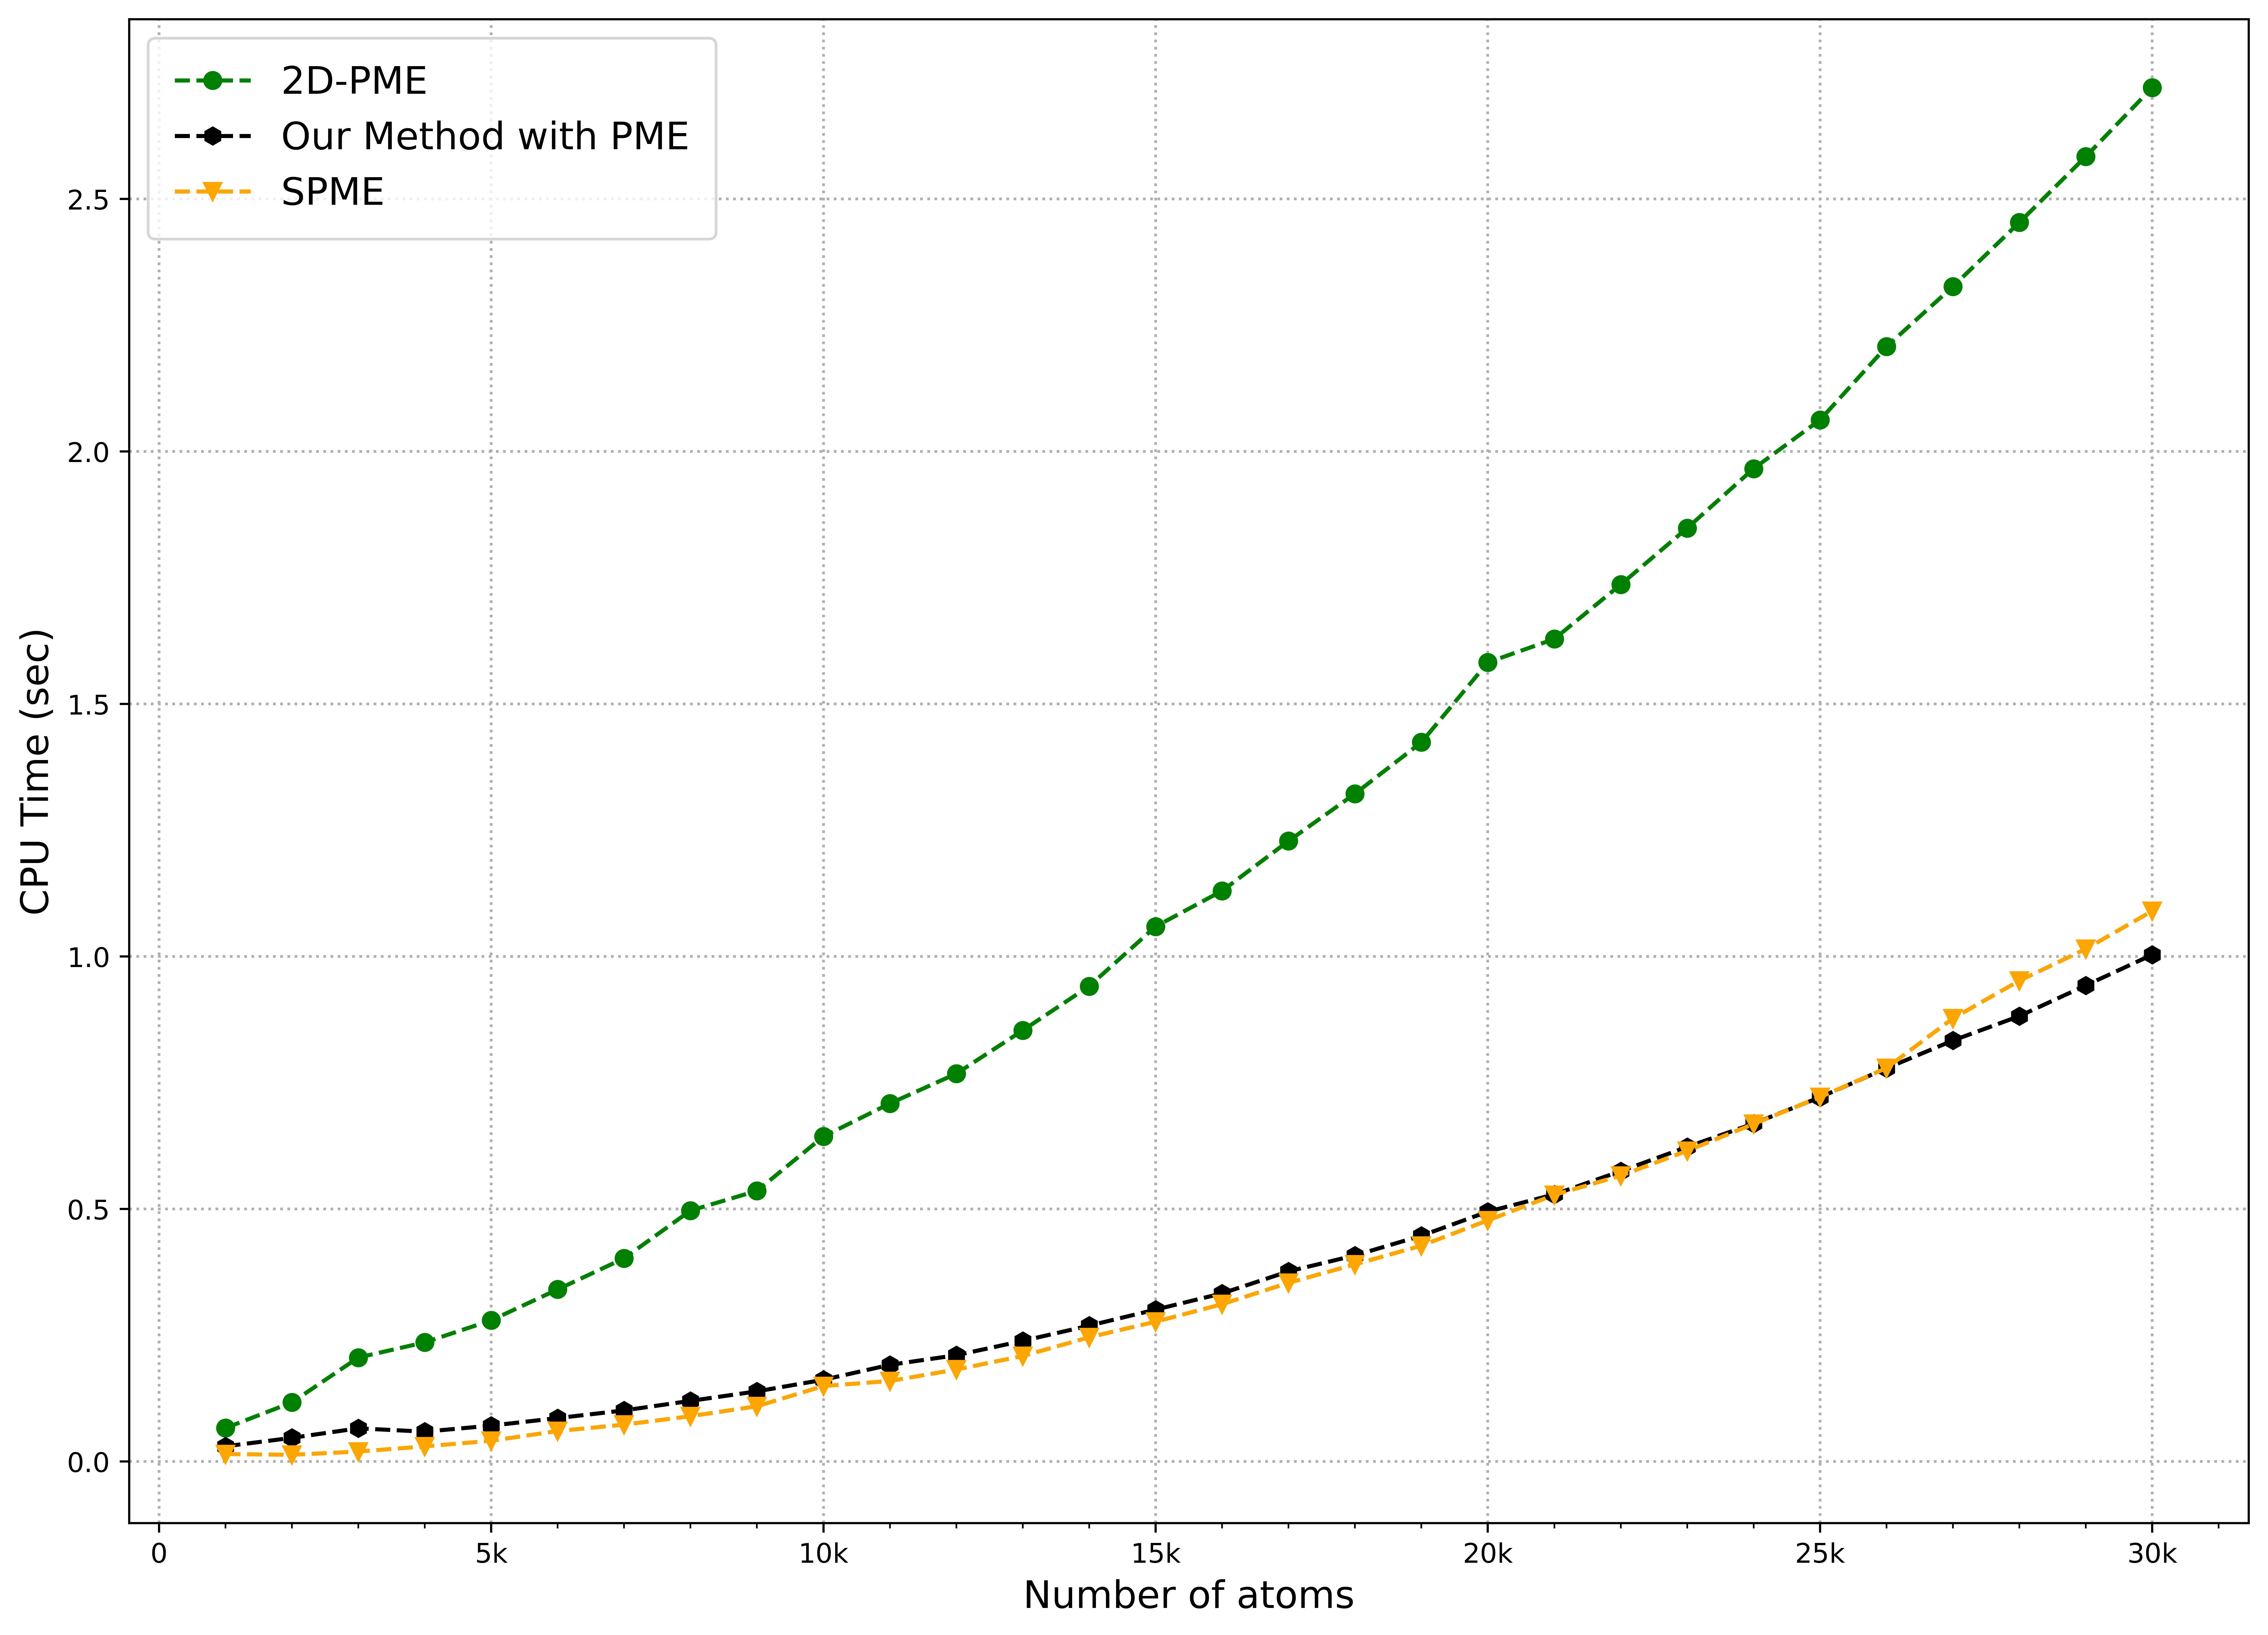
\includegraphics[width=\linewidth]{images/Scaling_behaviour_Result30k.jpg}
    \caption{Scaling behaviour of the computation time for total Ewald energies with increasing system size for the optimized PME implementation. The number of ions was varied from 1,000 to 30,000 while keeping the simulation box size fixed.  Our method demonstrated highly improved performance compared to the conventional \ac{2D-PME} approach and a similar performance to 3D-\ac{SPME}, using the same particle mesh configuration and achieving a comparable level of accuracy.}
    \label{fig:scaling_results}
\end{figure}
Our method shows a substantial improvement in computational efficiency compared to the conventional \ac{2D-PME} method. The scaling of the CPU time is significantly better as shown with the slower growth of the computational time in our method's curve. This enhanced performance can be attributed to the 3D-\ac{SPME} like formulation of our new method, which is evident as both show a similar performance. Since the 3D-SPME method is known for its scalability and accuracy, our implementation matches its performance while providing adaptability to slab-like geometries often encountered in biological and interfacial simulations. 
\chapter{Numerical Evaluation: Accuracy and Efficiency}
\label{Chapter5}
\lhead{Chapter 5. \emph{Numerical Evaluation: Accuracy and Efficiency}}

In this chapter, we present a comprehensive analysis of the performance of our newly proposed method with particular focus on its accuracy and efficiency. Through a series of computational experiments, we analyze how different parameters influence the quality of results and CPU-time performance. Specifically, we focus on convergence and the scaling behaviour of our method. All simulations were conducted on ionic systems of sodium (Na\textsuperscript{+}) and chloride (Cl\textsuperscript{-}) ions randomly distributed in a cubic box having a length of 25 \AA. These systems were modelled using the molecular dynamics package LAMMPS~\cite{LAMMPS}. The Ewald splitting parameter $\alpha$ was set to $5.42/L$ as recommended in several previous literature. @@@Please cite@@@

\section{Convergence and Accuracy of Reciprocal-Space Contributions with Varying $\gamma$}
In this section, we investigate how the reciprocal-space energy converges as the constant $\gamma$ is varied. A model system of 10000 ions was set up in a box with sides of length 25 \AA. As a benchmark, reference energies were computed using mathematically ``exact'' but computationally inefficient two-dimensional Ewald (2D-EW) method~\cite{kawata2001rapid}.
\subsection{The Role of $\gamma$}
The parameter $\gamma$ plays a central role in controlling the sharpness of the top-hat function that is introduced in the reciprocal sum of 3D Ewald summation method. The introduction of top-hat function filters the interactions arising from interaction of images in the z-direction.  In the new formulation, the long-range part of the Ewald summation is mathematically expressed as
\begin{flalign}
    (4\pi\epsilon_o)U^{LR}& =\frac{\sqrt{\pi}}{L_xL_y}\sum_{\vec{{k}}=-\infty}^{\infty}{}^\prime\left[ \int_{0}^{\alpha}\frac{dt}{t^2}C_{k_z}(t){exp}\left(\frac{-1}{4t^2}|\vec G|_{xy}^2\right)\right] |\,S(\vec G)\,|^2
\end{flalign}
here $\vec k$ = \{$k_x,k_y,k_z$\} and  the constant $\gamma$ appears in the function $C_{k_z}(t)$ given by
\begin{flalign}
     C_{k_z}(t) &=\frac{1}{L_z}\int_{-\infty}^{\infty}ds\hspace{1mm}exp(-i\frac{2\pi n s}{L_z})exp(-s^2t^2)\\
     &\times \left[\frac{1}{1+ exp(-\gamma(0.5L_z+s))} + \frac{1}{1+ exp(-\gamma(0.5L_z-s))} -1\right]
\end{flalign}

\begin{figure}[htbp]
    \centering
    \includegraphics[scale=0.4]{images/logerror_vs_kz_forreport.jpg}
    \caption{Convergence of relative errors in $U_{LR}$ with $k_z$ for various values of $\gamma$.}
    \label{fig:convergence_gamma}
\end{figure}

As shown in Fig.~(\ref{fig:convergence_gamma}) and discussed in Section~\ref{finding_gamma}, the use of different $\gamma$ values significantly influences the rate of convergence of the reciprocal-space energy. Larger $\gamma$ values lead to relatively faster convergence but introduce oscillatory behaviour in the energy estimates with low accuracy, contrary to smaller values, which have high accuracy and fewer oscillations. To achieve convergence in energies, one needs to reach a threshold $k_z$. Consequently, this brings a major drawback: for every additional iteration of $k_z$, the structure factor $S(\vec G)$~Eq.(\ref{eq:structurefactor}) is recomputed, which scales as $O(N)$@@@Please check this@@@, adding to the computational burden for high precision simulations. 

To eliminate this cost, we transition to the use of the Particle Mesh Ewald (PME) method, as formulated in Eq.~(\ref{eq:newreci2DSPME}). In this formulation, the most computationally expensive step becomes the charge interpolation on grids, which is executed only once and outside the main energy summation loop. As a result, the main energy summation loop is no longer the computational bottleneck, enabling significantly faster calculations without sacrificing accuracy.

\section{Implementation with Particle Mesh Ewald}
The Particle Mesh Ewald formulation introduces several additional parameters that directly impact both computational efficiency and numerical accuracy. They are the resolution of the mesh grid used for the Fast Fourier Transform (FFT) and the order of the B-spline interpolation for charge assignment. In this section, we systematically investigate how variations in these parameters affect the performance of our method, particularly in conjunction with different values of parameter $\gamma$.

In our modified implementation, we performed extensive tests across a variety of $\gamma$ values, grid sizes, and B-spline interpolation orders. For each configuration, we measured the accuracy of the computed electrostatic energy and recorded the CPU execution time. These combinations are presented in the Tables~\ref{tab:tablespme_gamma0p2}, \ref{tab:tablespme_gamma0p5}, \ref{tab:tablespme_gamma1}, \ref{tab:tablespme_gamma2p5}, and \ref{tab:tablespme_gamma10}

\begin{table}[H]
\centering
\begin{tabular}{|l|c|l|}
\hline
\textbf{Color Code}      & \textbf{Accuracy} & \textbf{Rel. Err. Range}                                      \\ \hline
\cellcolor[HTML]{F0F7DA} & Low               & More than $10^{-4}$                      \\ \hline
\cellcolor[HTML]{C9DF8A} & Medium            & Between $10^{-6}$ and $10^{-4}$ \\ \hline
\cellcolor[HTML]{77AB59} & High              & Less than $10^{-6}$                      \\ \hline
\end{tabular}
\caption{Color-coded accuracy classification for the SPME method based on error range}
\label{tab:accuracy-refer}
\end{table}
% high  77AB59
% mid C9DF8A
% low F0F7DA
\begin{table}[]
\centering
\caption{Particle Mesh Method: performance and accuracy for $\gamma = 0.2$.}
\label{tab:tablespme_gamma0p2}
\resizebox{\textwidth}{!}{%
\begin{tabular}{cccccc}
\hline
\multicolumn{1}{|c|}{{Order$_{xy}$}} &
  \multicolumn{1}{c|}{{Order$_z$}} &
  \multicolumn{1}{c|}{{Grid$_{xy}$}} &
  \multicolumn{1}{c|}{{Grid$_z$}} &
  \multicolumn{1}{c|}{{\begin{tabular}[c]{@{}c@{}}CPU-Time\\ (sec)\end{tabular}}} &
  \multicolumn{1}{c|}{{\begin{tabular}[c]{@{}c@{}}Rel. Err.\\ Energy\end{tabular}}} \\ \hline
\rowcolor[HTML]{F0F7DA} 
4  & 4  & 16 & 512 & 0.0748 & 4.4E-04 \\
\rowcolor[HTML]{C9DF8A} 
4  & 4  & 32 & 512 & 0.0805 & 4.2E-05 \\
\rowcolor[HTML]{C9DF8A} 
4  & 4  & 64 & 512 & 0.1076 & 1.8E-05 \\
\rowcolor[HTML]{F0F7DA} 
4  & 6  & 16 & 512 & 0.0751 & 4.2E-04 \\
\rowcolor[HTML]{C9DF8A} 
4  & 6  & 32 & 512 & 0.0807 & 2.6E-05 \\
\rowcolor[HTML]{C9DF8A} 
4  & 6  & 64 & 512 & 0.1090 & 1.8E-06 \\
\rowcolor[HTML]{F0F7DA} 
4  & 8  & 16 & 512 & 0.0810 & 4.2E-04 \\
\rowcolor[HTML]{C9DF8A} 
4  & 8  & 32 & 512 & 0.0868 & 2.6E-05 \\
\rowcolor[HTML]{C9DF8A} 
4  & 8  & 64 & 512 & 0.1162 & 1.7E-06 \\
\rowcolor[HTML]{F0F7DA} 
4  & 10 & 16 & 512 & 0.1060 & 4.2E-04 \\
\rowcolor[HTML]{C9DF8A} 
4  & 10 & 32 & 512 & 0.1118 & 2.6E-05 \\
\rowcolor[HTML]{C9DF8A} 
4  & 10 & 64 & 512 & 0.1391 & 1.7E-06 \\
\rowcolor[HTML]{C9DF8A} 
6  & 6  & 16 & 512 & 0.1260 & 1.3E-05 \\
\rowcolor[HTML]{77AB59} 
6  & 6  & 32 & 512 & 0.1328 & 4.0E-07 \\
\rowcolor[HTML]{77AB59} 
6  & 6  & 64 & 512 & 0.1709 & 2.7E-07 \\
\rowcolor[HTML]{C9DF8A} 
6  & 8  & 16 & 512 & 0.1322 & 1.3E-05 \\
\rowcolor[HTML]{77AB59} 
6  & 8  & 32 & 512 & 0.1401 & 3.0E-07 \\
\rowcolor[HTML]{77AB59} 
6  & 8  & 64 & 512 & 0.1788 & 1.7E-07 \\
\rowcolor[HTML]{C9DF8A} 
6  & 10 & 16 & 512 & 0.1580 & 1.3E-05 \\
\rowcolor[HTML]{77AB59} 
6  & 10 & 32 & 512 & 0.1637 & 3.0E-07 \\
\rowcolor[HTML]{77AB59} 
6  & 10 & 64 & 512 & 0.2027 & 1.7E-07 \\
\rowcolor[HTML]{77AB59} 
8  & 8  & 32 & 512 & 0.2182 & 1.7E-07 \\
\rowcolor[HTML]{77AB59} 
8  & 8  & 64 & 512 & 0.2701 & 1.7E-07 \\
\rowcolor[HTML]{77AB59} 
8  & 10 & 32 & 512 & 0.2444 & 1.7E-07 \\
\rowcolor[HTML]{77AB59} 
8  & 10 & 64 & 512 & 0.2999 & 1.6E-07 \\
\rowcolor[HTML]{77AB59} 
10 & 10 & 64 & 512 & 0.4521 & 1.6E-07
\end{tabular}%
}
\end{table}
% high  77AB59
% mid C9DF8A
% low F0F7DA
\begin{table}[]
\centering
\caption{Particle Mesh Method: performance and accuracy for $\gamma = 0.5$.}
\label{tab:tablespme_gamma0p5}
\resizebox{\textwidth}{!}{%
\begin{tabular}{cccccc}
\hline
\multicolumn{1}{|c|}{{Order$_{xy}$}} &
  \multicolumn{1}{c|}{{Order$_z$}} &
  \multicolumn{1}{c|}{{Grid$_{xy}$}} &
  \multicolumn{1}{c|}{{Grid$_z$}} &
  \multicolumn{1}{c|}{{\begin{tabular}[c]{@{}c@{}}CPU-Time\\ (sec)\end{tabular}}} &
  \multicolumn{1}{c|}{{\begin{tabular}[c]{@{}c@{}}Rel. Err.\\ Energy\end{tabular}}} \\ \hline
\rowcolor[HTML]{F0F7DA} 
4  & 4  & 16  & 256 & 0.0426 & 4.4E-04 \\
\rowcolor[HTML]{C9DF8A} 
4  & 4  & 32  & 256 & 0.0465 & 4.0E-05 \\
\rowcolor[HTML]{C9DF8A} 
4  & 4  & 64  & 256 & 0.0599 & 1.5E-05 \\
\rowcolor[HTML]{F0F7DA} 
4  & 6  & 16  & 256 & 0.0436 & 4.2E-04 \\
\rowcolor[HTML]{C9DF8A} 
4  & 6  & 32  & 256 & 0.0479 & 2.6E-05 \\
\rowcolor[HTML]{C9DF8A} 
4  & 6  & 64  & 256 & 0.0611 & 1.7E-06 \\
\rowcolor[HTML]{F0F7DA} 
4  & 8  & 16  & 256 & 0.0497 & 4.2E-04 \\
\rowcolor[HTML]{C9DF8A} 
4  & 8  & 32  & 256 & 0.0539 & 2.6E-05 \\
\rowcolor[HTML]{C9DF8A} 
4  & 8  & 64  & 256 & 0.0667 & 1.6E-06 \\
\rowcolor[HTML]{F0F7DA} 
4  & 10 & 16  & 256 & 0.0742 & 4.2E-04 \\
\rowcolor[HTML]{C9DF8A} 
4  & 10 & 32  & 256 & 0.0783 & 2.6E-05 \\
\rowcolor[HTML]{C9DF8A} 
4  & 10 & 64  & 256 & 0.0914 & 1.6E-06 \\
\rowcolor[HTML]{C9DF8A} 
6  & 6  & 16  & 256 & 0.0720 & 1.3E-05 \\
\rowcolor[HTML]{77AB59} 
6  & 6  & 32  & 256 & 0.0767 & 2.9E-07 \\
\rowcolor[HTML]{77AB59} 
6  & 6  & 64  & 256 & 0.0923 & 1.6E-07 \\
\rowcolor[HTML]{C9DF8A} 
6  & 8  & 16  & 256 & 0.0788 & 1.3E-05 \\
\rowcolor[HTML]{77AB59} 
6  & 8  & 32  & 256 & 0.0833 & 2.2E-07 \\
\rowcolor[HTML]{77AB59} 
6  & 8  & 64  & 256 & 0.0968 & 8.7E-08 \\
\rowcolor[HTML]{C9DF8A} 
6  & 10 & 16  & 256 & 0.1038 & 1.3E-05 \\
\rowcolor[HTML]{77AB59} 
6  & 10 & 32  & 256 & 0.1074 & 2.2E-07 \\
\rowcolor[HTML]{77AB59} 
6  & 10 & 64  & 256 & 0.1234 & 8.6E-08 \\
\rowcolor[HTML]{77AB59} 
8  & 8  & 32  & 256 & 0.1319 & 8.6E-08 \\
\rowcolor[HTML]{77AB59} 
8  & 8  & 64  & 256 & 0.1489 & 8.5E-08 \\
\rowcolor[HTML]{77AB59} 
8  & 10 & 32  & 256 & 0.1555 & 8.6E-08 \\
\rowcolor[HTML]{77AB59} 
8  & 10 & 64  & 256 & 0.1782 & 8.4E-08 \\
\rowcolor[HTML]{77AB59} 
10 & 10 & 128 & 256 & 0.3718 & 8.4E-08
\end{tabular}%
}
\end{table}
% high  77AB59
% mid C9DF8A
% low F0F7DA
\begin{table}[]
\centering
\caption{Particle Mesh Method: performance and accuracy for $\gamma = 1.0$.}
\label{tab:tablespme_gamma1}
\resizebox{\textwidth}{!}{%
\begin{tabular}{cccccc}
\hline
\multicolumn{1}{|c|}{{Order$_{xy}$}} &
  \multicolumn{1}{c|}{{Order$_z$}} &
  \multicolumn{1}{c|}{{Grid$_{xy}$}} &
  \multicolumn{1}{c|}{{Grid$_z$}} &
  \multicolumn{1}{c|}{{\begin{tabular}[c]{@{}c@{}}CPU-Time\\ (sec)\end{tabular}}} &
  \multicolumn{1}{c|}{{\begin{tabular}[c]{@{}c@{}}Rel. Err.\\ Energy\end{tabular}}} \\ \hline
\rowcolor[HTML]{F0F7DA} 
4  & 4  & 16 & 128 & 0.0262 & 4.6E-04 \\
\rowcolor[HTML]{C9DF8A} 
4  & 4  & 32 & 128 & 0.0294 & 6.5E-05 \\
\rowcolor[HTML]{C9DF8A} 
4  & 4  & 64 & 128 & 0.0373 & 4.1E-05 \\
\rowcolor[HTML]{F0F7DA} 
4  & 6  & 16 & 128 & 0.0276 & 4.2E-04 \\
\rowcolor[HTML]{C9DF8A} 
4  & 6  & 32 & 128 & 0.0308 & 2.6E-05 \\
\rowcolor[HTML]{C9DF8A} 
4  & 6  & 64 & 128 & 0.0387 & 2.0E-06 \\
\rowcolor[HTML]{F0F7DA} 
4  & 8  & 16 & 128 & 0.0337 & 4.2E-04 \\
\rowcolor[HTML]{C9DF8A} 
4  & 8  & 32 & 128 & 0.0369 & 2.6E-05 \\
\rowcolor[HTML]{C9DF8A} 
4  & 8  & 64 & 128 & 0.0447 & 1.6E-06 \\
\rowcolor[HTML]{F0F7DA} 
4  & 10 & 16 & 128 & 0.0586 & 4.2E-04 \\
\rowcolor[HTML]{C9DF8A} 
4  & 10 & 32 & 128 & 0.0614 & 2.6E-05 \\
\rowcolor[HTML]{C9DF8A} 
4  & 10 & 64 & 128 & 0.0693 & 1.6E-06 \\
\rowcolor[HTML]{C9DF8A} 
6  & 6  & 16 & 128 & 0.0452 & 1.3E-05 \\
\rowcolor[HTML]{77AB59} 
6  & 6  & 32 & 128 & 0.0481 & 6.1E-07 \\
\rowcolor[HTML]{77AB59} 
6  & 6  & 64 & 128 & 0.0564 & 4.8E-07 \\
\rowcolor[HTML]{C9DF8A} 
6  & 8  & 16 & 128 & 0.0517 & 1.3E-05 \\
\rowcolor[HTML]{77AB59} 
6  & 8  & 32 & 128 & 0.0546 & 2.3E-07 \\
\rowcolor[HTML]{77AB59} 
6  & 8  & 64 & 128 & 0.0626 & 9.9E-08 \\
\rowcolor[HTML]{C9DF8A} 
6  & 10 & 16 & 128 & 0.0761 & 1.3E-05 \\
\rowcolor[HTML]{77AB59} 
6  & 10 & 32 & 128 & 0.0802 & 2.3E-07 \\
\rowcolor[HTML]{77AB59} 
6  & 10 & 64 & 128 & 0.0876 & 9.2E-08 \\
\rowcolor[HTML]{77AB59} 
8  & 8  & 32 & 128 & 0.0859 & 9.8E-08 \\
\rowcolor[HTML]{77AB59} 
8  & 8  & 64 & 128 & 0.0942 & 9.7E-08 \\
\rowcolor[HTML]{77AB59} 
8  & 10 & 32 & 128 & 0.1105 & 9.2E-08 \\
\rowcolor[HTML]{77AB59} 
8  & 10 & 64 & 128 & 0.1194 & 9.1E-08 \\
\rowcolor[HTML]{77AB59} 
10 & 10 & 64 & 128 & 0.1941 & 9.1E-08
\end{tabular}%
}
\end{table}
% high  77AB59
% mid C9DF8A
% low F0F7DA
\begin{table}[]
\centering
\caption{Particle Mesh Method: performance and accuracy for $\gamma = 2.5$.}
\label{tab:tablespme_gamma2p5}
\resizebox{\textwidth}{!}{%
\begin{tabular}{cccccc}
\hline
\multicolumn{1}{|c|}{{Order$_{xy}$}} &
  \multicolumn{1}{c|}{{Order$_z$}} &
  \multicolumn{1}{c|}{{Grid$_{xy}$}} &
  \multicolumn{1}{c|}{{Grid$_z$}} &
  \multicolumn{1}{c|}{{\begin{tabular}[c]{@{}c@{}}CPU-Time\\ (sec)\end{tabular}}} &
  \multicolumn{1}{c|}{{\begin{tabular}[c]{@{}c@{}}Rel. Err.\\ Energy\end{tabular}}} \\ \hline
\rowcolor[HTML]{F0F7DA} 
4  & 4  & 16 & 128 & 0.0276  & 4.3E-04 \\
\rowcolor[HTML]{C9DF8A} 
4  & 4  & 32 & 128 & 0.0313  & 3.3E-05 \\
\rowcolor[HTML]{C9DF8A} 
4  & 4  & 64 & 128 & 0.0396  & 9.1E-06 \\
\rowcolor[HTML]{F0F7DA} 
4  & 8  & 16 & 128 & 0.0357  & 4.3E-04 \\
\rowcolor[HTML]{C9DF8A} 
4  & 8  & 32 & 128 & 0.0388  & 2.7E-05 \\
\rowcolor[HTML]{C9DF8A} 
4  & 8  & 64 & 128 & 0.0478  & 3.1E-06 \\
\rowcolor[HTML]{F0F7DA} 
4  & 10 & 16 & 128 & 0.0613  & 4.3E-04 \\
\rowcolor[HTML]{C9DF8A} 
4  & 10 & 32 & 128 & 0.0653  & 2.7E-05 \\
\rowcolor[HTML]{C9DF8A} 
4  & 10 & 64 & 128 & 0.0722  & 3.1E-06 \\
\rowcolor[HTML]{C9DF8A} 
6  & 8  & 16 & 128 & 0.0534  & 1.5E-05 \\
\rowcolor[HTML]{C9DF8A} 
6  & 8  & 32 & 128 & 0.0567  & 1.7E-06 \\
\rowcolor[HTML]{C9DF8A} 
6  & 8  & 64 & 128 & 0.0652  & 1.5E-06 \\
\rowcolor[HTML]{C9DF8A} 
6  & 10 & 16 & 128 & 0.0798  & 1.5E-05 \\
\rowcolor[HTML]{C9DF8A} 
6  & 10 & 32 & 128 & 0.0824  & 1.7E-06 \\
\rowcolor[HTML]{C9DF8A} 
6  & 10 & 64 & 128 & 0.0909  & 1.5E-06 \\
\rowcolor[HTML]{C9DF8A} 
8  & 8  & 32 & 128 & 0.0936  & 1.5E-06 \\
\rowcolor[HTML]{C9DF8A} 
8  & 8  & 64 & 128 & 0.1037  & 1.5E-06 \\
\rowcolor[HTML]{C9DF8A} 
8  & 10 & 64 & 128 & 0.12805 & 1.5E-06 \\
\rowcolor[HTML]{C9DF8A} 
10 & 10 & 64 & 128 & 0.20766 & 1.5E-06
\end{tabular}%
}
\end{table}
% high  77AB59
% mid C9DF8A
% low F0F7DA
\begin{table}[]
\centering
\caption{Particle Mesh Method: performance and accuracy for $\gamma = 10$.}
\label{tab:tablespme_gamma10}
\resizebox{\textwidth}{!}{%
\begin{tabular}{cccccc}
\hline
\multicolumn{1}{|c|}{{Order$_{xy}$}} &
  \multicolumn{1}{c|}{{Order$_z$}} &
  \multicolumn{1}{c|}{{Grid$_{xy}$}} &
  \multicolumn{1}{c|}{{Grid$_z$}} &
  \multicolumn{1}{c|}{{\begin{tabular}[c]{@{}c@{}}CPU-Time\\ (sec)\end{tabular}}} &
  \multicolumn{1}{c|}{{\begin{tabular}[c]{@{}c@{}}Rel. Err.\\ Energy\end{tabular}}} \\ \hline
\rowcolor[HTML]{F0F7DA} 
4  & 4  & 16 & 128 & 0.0276 & 4.8E-04 \\
\rowcolor[HTML]{C9DF8A} 
4  & 4  & 32 & 128 & 0.0309 & 8.1E-05 \\
\rowcolor[HTML]{C9DF8A} 
4  & 4  & 64 & 128 & 0.0389 & 5.6E-05 \\
\rowcolor[HTML]{F0F7DA} 
4  & 8  & 16 & 128 & 0.0358 & 4.8E-04 \\
\rowcolor[HTML]{C9DF8A} 
4  & 8  & 64 & 128 & 0.0476 & 5.5E-05 \\
\rowcolor[HTML]{F0F7DA} 
4  & 10 & 16 & 128 & 0.0618 & 4.8E-04 \\
\rowcolor[HTML]{C9DF8A} 
4  & 10 & 64 & 128 & 0.0734 & 5.4E-05 \\
\rowcolor[HTML]{C9DF8A} 
6  & 8  & 64 & 128 & 0.0675 & 5.3E-05 \\
\rowcolor[HTML]{C9DF8A} 
6  & 10 & 64 & 128 & 0.0939 & 5.3E-05 \\
\rowcolor[HTML]{C9DF8A} 
8  & 8  & 64 & 128 & 0.1025 & 5.3E-05 \\
\rowcolor[HTML]{C9DF8A} 
8  & 10 & 64 & 128 & 0.1284 & 5.3E-05 \\
\rowcolor[HTML]{C9DF8A} 
10 & 10 & 64 & 128 & 0.2109 & 5.3E-05
\end{tabular}%
}
\end{table}

Several general trends emerged from the analysis. Lower values of $\gamma$ were found to require finer grids in the $ z$-direction in order to achieve a comparable level of accuracy, which in turn increases the computational cost. Increasing the B-spline interpolation order generally improves the accuracy of the energy calculations; however, that effect diminishes beyond a certain order while the computational overhead continues to increase. While multiple configurations may yield acceptable results, the combination of $\gamma = 1$, a grid size of $64 \times 64 \times 128$, and a B-spline interpolation order of 8 was found to offer the most favourable balance between numerical accuracy and computational efficiency among the cases evaluated.

\section{Scaling Behaviour with System Size}
To evaluate the scalability of our method with respect to system size, we analyzed the computational performance of the PME implementation of our method. The number of ions was varied from 1,000 to 30,000, with particle positions randomly distributed within a fixed simulation box. Throughout all simulations, the PME configuration was kept uniform with a grid size of $64 \times 64 \times 128$, a B-spline interpolation order of 8, and parameter $\gamma = 1$, as identified in the previous section. For comparison, we also included results from previously established methods based on 2D and 3D periodic boundary conditions, with particle mesh adaptation for a similar level of accuracy. The scaling behaviour of the total computation time with increasing system size is shown in Fig.~(\ref{fig:scaling_results}). 
\begin{figure}[]
    \centering
    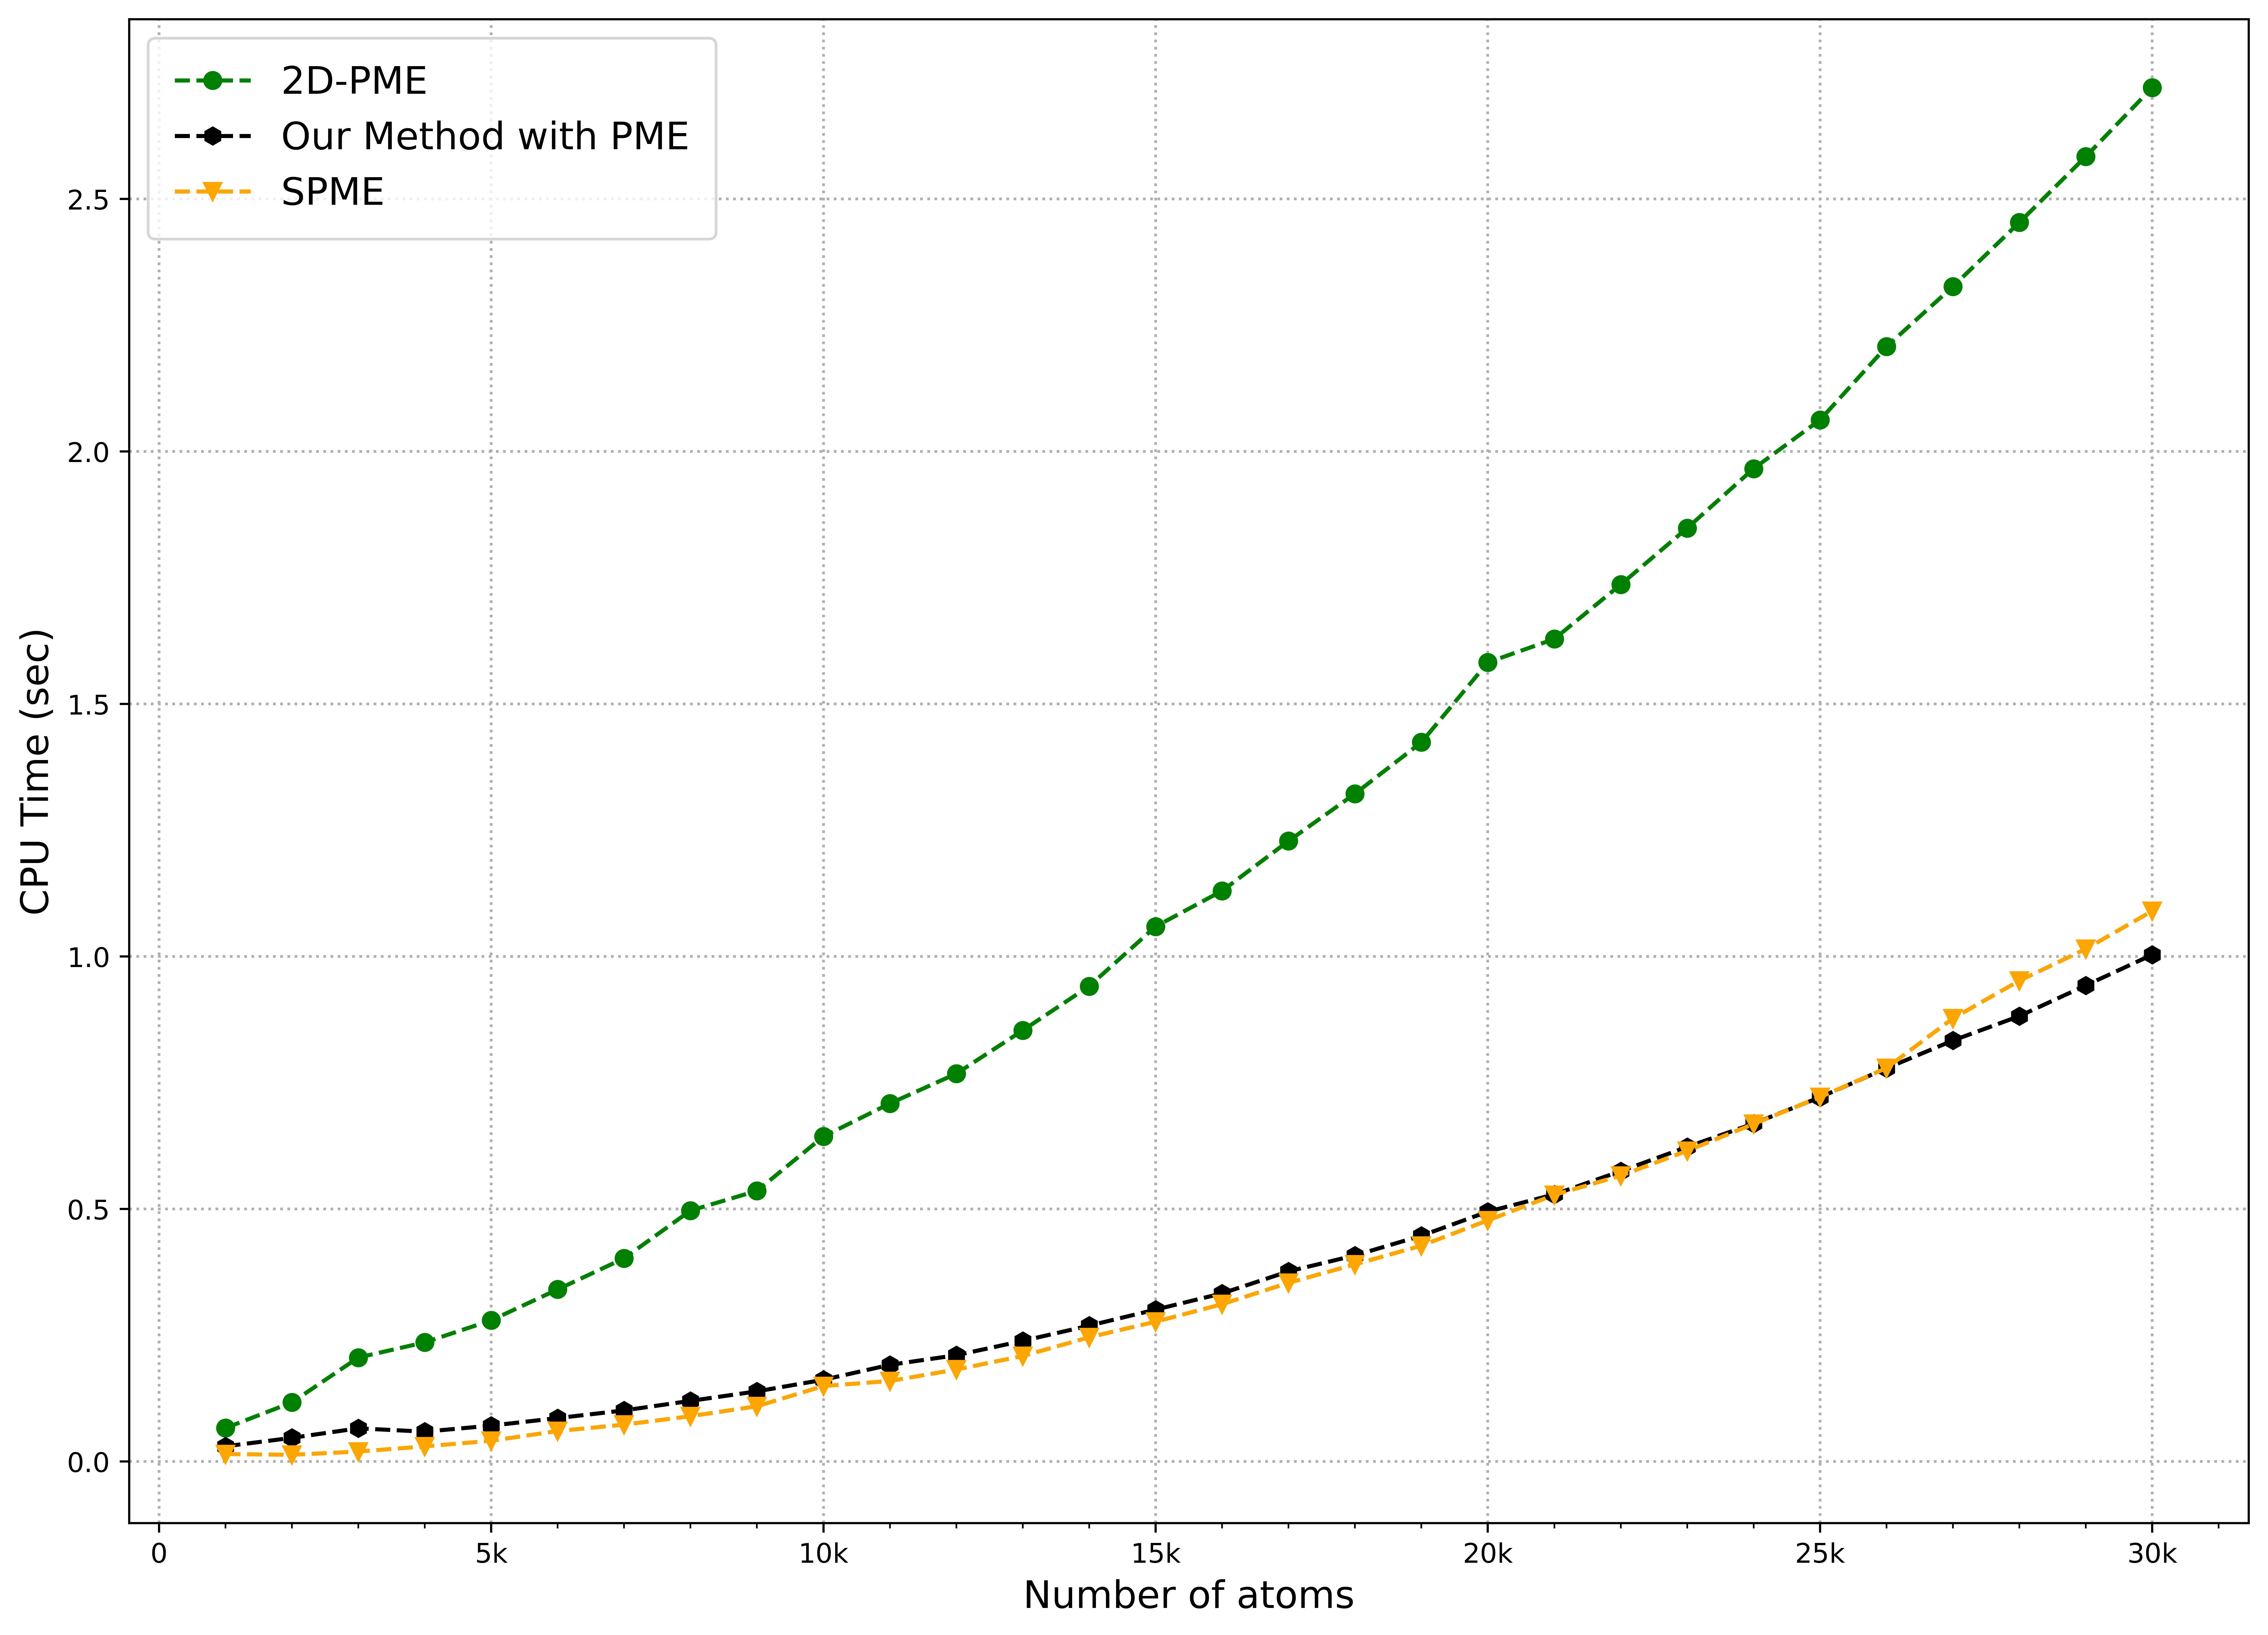
\includegraphics[width=\linewidth]{images/Scaling_behaviour_Result30k.jpg}
    \caption{Scaling behaviour of the computation time for total Ewald energies with increasing system size for the optimized PME implementation. The number of ions was varied from 1,000 to 30,000 while keeping the simulation box size fixed.  Our method demonstrated highly improved performance compared to the conventional 2D-PME approach and a similar performance to 3D-\ac{SPME}, using the same particle mesh configuration and achieving a comparable level of accuracy.}
    \label{fig:scaling_results}
\end{figure}
Our method shows a substantial improvement in computational efficiency compared to the conventional \ac{2D-PME} method. The scaling of the CPU Time is significantly better as shown with the slower growth of the computational time in our method's curve. This enhanced performance can be attributed to the 3D-\ac{SPME} like formulation of our new method, which is evident as both show a similar performance. Since the 3D-SPME method is known for its scalability and accuracy, our implementation matches its performance while providing adaptability to slab-like geometries often encountered in biological and interfacial simulations. This major performance improvement opens the door for simulations of larger biomolecular systems or extended time scales without compromising accuracy or efficiency.
% Chapter Template

\chapter{Performance Analysis and Optimization}

\label{Chapter6}

\lhead{Chapter 6. \emph{Performance Analysis and Optimization}}
After implementing the new 2D Ewald summation algorithm, the subsequent objective was to identify performance bottlenecks in the program, as the next critical step in guiding further optimization efforts. Intel VTune Profiler was used for this purpose, as it provides detailed insights into the program’s execution by highlighting time-consuming functions, and parallelization inefficiencies.
% \section{Performance Analysis using Intel VTune Profiler}
\section{Baseline Program}
Hotspot analysis of the program was performed to identify computational bottlenecks. The results in Fig.~(\ref{fig:result1vtune}), indicate that the real-space component accounts for approximately 60-65\% of the total CPU time. The most expensive function was \texttt{dist}, responsible for inter-particle distance calculations, consuming around 25\% of the execution time. This cost is compounded by repeated calls to the \texttt{\_\_erfc} function from \texttt{libm-2.31.so}, contributing approximately 20\% of the total runtime. These findings highlight the need to optimize the real-space calculations, particularly the error function evaluation, to improve overall performance.
% \begin{figure}[htbp]
\begin{figure}[H]
    \centering
    \begin{minipage}{0.7\textwidth}
        \fbox{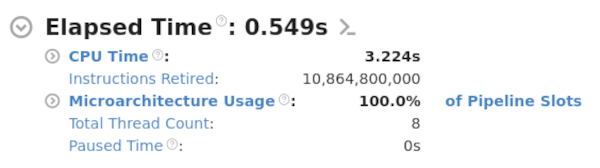
\includegraphics[width=\linewidth]{images/VTuneInitialTime.png}}
    \end{minipage}%
    \begin{minipage}{0.3\textwidth}
        \caption{Execution time details for baseline program.}
    \end{minipage}
\end{figure}
% \begin{figure}[htbp]
\begin{figure}[H]
    \centering
    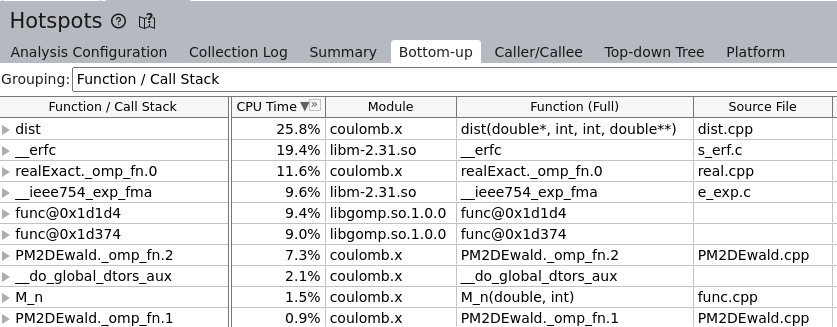
\includegraphics[width = \linewidth]{images/VTuneInitialHotspot.png}
    \caption{Hotspot analysis of the baseline Ewald summation implementation, as reported by Intel VTune Profiler. A significant portion of total CPU time is concentrated in the \textit{dist} function (25.8\%), the standard math library's \textit{\_\_erfc} function (19.4\%).}
    \label{fig:result1vtune}
\end{figure}

\section{Polynomial Interpolation of Error Function}
A significant portion of the program’s execution time was consumed by calls to the \verb|std::erfc| function. To reduce the computational cost associated with evaluating the complementary error function \(\operatorname{erfc}(x)\) in the real-space part of the Ewald summation, a polynomial interpolation approach was adopted. This technique is outlined in \textit{Handbook of Mathematical Functions by Abramowitz and Stegun (1964)}. The expression used is
\begin{equation}  
    erf(x) = 1 - (a_1 t + a_2 t^2 + a_3 t^3 + a_4 t^4 + a_5 t^5) e^{-x^2} + \epsilon(x)
\end{equation}
\[
    t = \frac{1}{1 + px}, \quad |\epsilon(x)| \leq 1.5 \times 10^{-7},
\]
\[
p = 0.3275911, \\
a_1 = 0.254829592, \\
a_2 = -0.284496736,
\]
\[
a_3 = 1.421413741, \\
a_4 = -1.453152027, \\
a_5 = 1.061405429.
\]
The polynomial was subsequently adapted as a replacement for the standard $\operatorname{erfc}(x)$ function in the real-space evaluation. This approach is advantageous because $\operatorname{erfc}(x)$ is computationally more expensive than $\operatorname{exp}(x)$. The evaluation of $\operatorname{erfc}(x)$ requires complex numerical approximations to compute an integral that does not have a simple closed form. In contrast, $\operatorname{exp}(x)$ is simpler, optimized, and often directly supported by hardware, which makes it significantly faster to compute.

\section{Additional Optimizations}
\subsection{Array Flattening}
In the implementation, data involving multiple dimensions must be stored in several parts of the program, such as atom positions and charge spreading array for the SPME. While multidimensional arrays are a natural choice for such data, they have drawbacks. 

Dynamically allocated multidimensional arrays often lead to scattered memory layouts and multiple pointer dereferences. This results in poor cache performance and added complexity in memory management. 
To address this, a one-dimensional array was used to represent the multidimensional structure. For an array with rank $d$ and dimensions $n_1\times \ldots \times n_d$, an element at ($i_1\times \ldots \times i_d$) maps to:
\begin{flalign*}
    i_d + n_d \cdot \left( i_{d-1} + n_{d-1} \cdot \left( \ldots + n_2 \cdot i_1 \right)\right)
\end{flalign*}
This approach reduced overhead, improved memory locality, and allowed faster access through direct indexing.
\subsection{Vectorization}
Vectorization enables the simultaneous processing of multiple data elements using a single instruction. This approach significantly improves both the speed and efficiency of computations. It is a fundamental technique in high-performance numerical computing, scientific simulations, graphics, and machine learning, as it leverages the SIMD (Single Instruction Multiple Data) capabilities present in modern processors.

In this work, the program has been compiled using the flags \texttt{-O3}, \texttt{-mavx2}, \texttt{-march=native}, \texttt{-ftree-vectorize}, and \texttt{-ftree-vectorizer-verbose=1}. The \texttt{-O3} flag enables aggressive optimization, including automatic vectorization of loops. The \texttt{-mavx2} flag ensures that the generated code utilizes AVX2 instructions, which operate on 256-bit registers. This allows the simultaneous processing of 8 single-precision floating-point numbers or 4 double-precision floating-point numbers, thereby greatly accelerating loops and computation-intensive sections of the code.

\section{Optimized Implementation}
% \section{Performance of Optimized Implementation}
Following the improvements, hotspot analysis of the optimized implementation Fig.~(\ref{fig:resultVTuneFinal}), shows a notable shift in the computational profile. The \texttt{\_\_erfc} function no longer appears among the major hotspots. The primary contributors to CPU time are now \texttt{dist} (35.4\%) and \texttt{real\_omp\_fn.0} (23.2\%), both associated with real-space computations. 
% Detailed performance improvements are presented in the \textit{Numerical Analysis} section of the thesis.
\begin{figure}[htbp]
% \begin{figure}[]
    \centering
    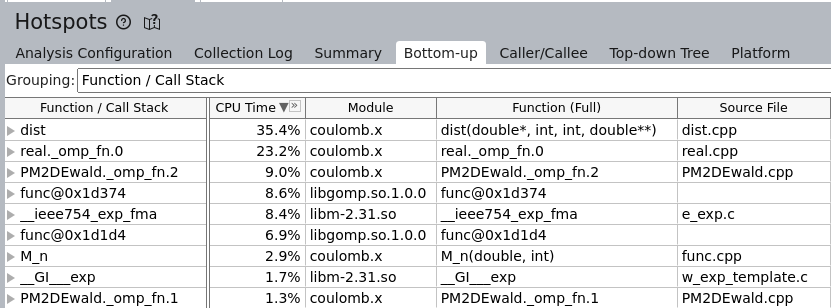
\includegraphics[width = \linewidth]{images/VTuneFinalHotSpots.png}
    \caption{Hotspot analysis of the optimized Ewald summation implementation, using a polynomial interpolation for the error function. The overall CPU time distribution indicates improved efficiency in the real-space term.}
    \label{fig:resultVTuneFinal}
\end{figure}
\begin{figure}[htbp]
% \begin{figure}[]
    \centering
    \begin{minipage}{0.7\textwidth}
        \fbox{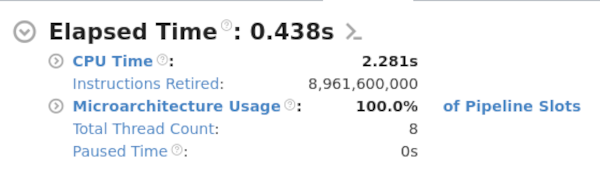
\includegraphics[width=\linewidth]{images/VTuneFinalTime.png}}
    \end{minipage}%
    \begin{minipage}{0.3\textwidth}
        \caption{Execution time details for improved program.}
    \end{minipage}
\end{figure}

\section{Parallelization}
Parallel programming can have an enormous impact on the performance and scalability of computational applications. The motivation for parallelizing a code is to reduce its execution time, enabling it to run faster on modern multiprocessor systems. In this context, the Ewald summation algorithm is crucial, as it is computationally intensive. Depending on the specific component of the calculation, its computational complexity ranges from $O(N^2)$ to $O(NlogN)$, making it essential to accelerate through parallel techniques. Efficient parallelization is critical for simulating long-range interactions in order to study large-scale systems.

\subsection{OpenMP}
In Ewald summation, the majority of the execution time is spent in running \texttt{for} loops. These loops are best suited for parallelization using OpenMP, which can effectively distribute the workload across multiple threads to improve performance.

OpenMP is a shared-memory parallel programming standard that allows for step-by-step parallelization. It requires only minor changes to the original sequential code, making it easy to apply. Unlike other methods that need a supercomputer, OpenMP can provide speed-up even on personal computers with two or more processor cores.

\subsection{Implementation Details}
\textbf{Reduction:} The \verb|reduction| clause is used to safely accumulate the result of a shared variable such as the real or the reciprocal energies. Each thread maintains a private copy of the reduction variable and they automatically combine that at the end of the parallel region using the specified reduction operator. An example of its application in the reciprocal space energy calculation is shown below
\lstinputlisting[language=C]{CodeFiles/reduction.c}

\textbf{Race condition during charge spreading:} A naïve approach that assigns one thread to map each charge onto the grid can lead to synchronization issues when multiple threads attempt to update the same grid point. During the computation of the charge spreading array $Q$, overlapping interpolation regions may cause several threads to modify the same grid location at the same time, resulting in a race condition and potentially incorrect values. To handle this, the \verb|atomic update| clause in OpenMP was used to ensure that updates are performed atomically, thereby preventing simultaneous read and write operations by different threads.
\lstinputlisting[language=C]{CodeFiles/atomic.c}

\textbf{Nested loops:} To parallelize the independent nested loops involved in the reciprocal space summation over the three-dimensional grids, the \texttt{collapse(3)} clause is employed. This directive flattens the nested loops into a single iteration space, thereby enhancing load balancing and facilitating uniform distribution of the computational workload across threads.
\lstinputlisting[language=C]{CodeFiles/collapse.c}

\subsection{Performance Evaluation}
To assess the effectiveness of OpenMP based parallelization, a series of calculations were performed for varying system sizes. The execution times were recorded by varying the number of OpenMP threads from 1 to 23, examining the scalability of the program. The experiments were performed on a machine with a 12\textsuperscript{th} Gen Intel\textsuperscript{\textregistered} Core\texttrademark{} i5-12500~$\times$~12 core processor. The operating system was OpenSUSE 15.5. The compiler was GCC 7.5.0.

\begin{figure}[H]
    \centering
    \subfigure[Total simulation time for different thread counts for direct Ewald summation.]{%
        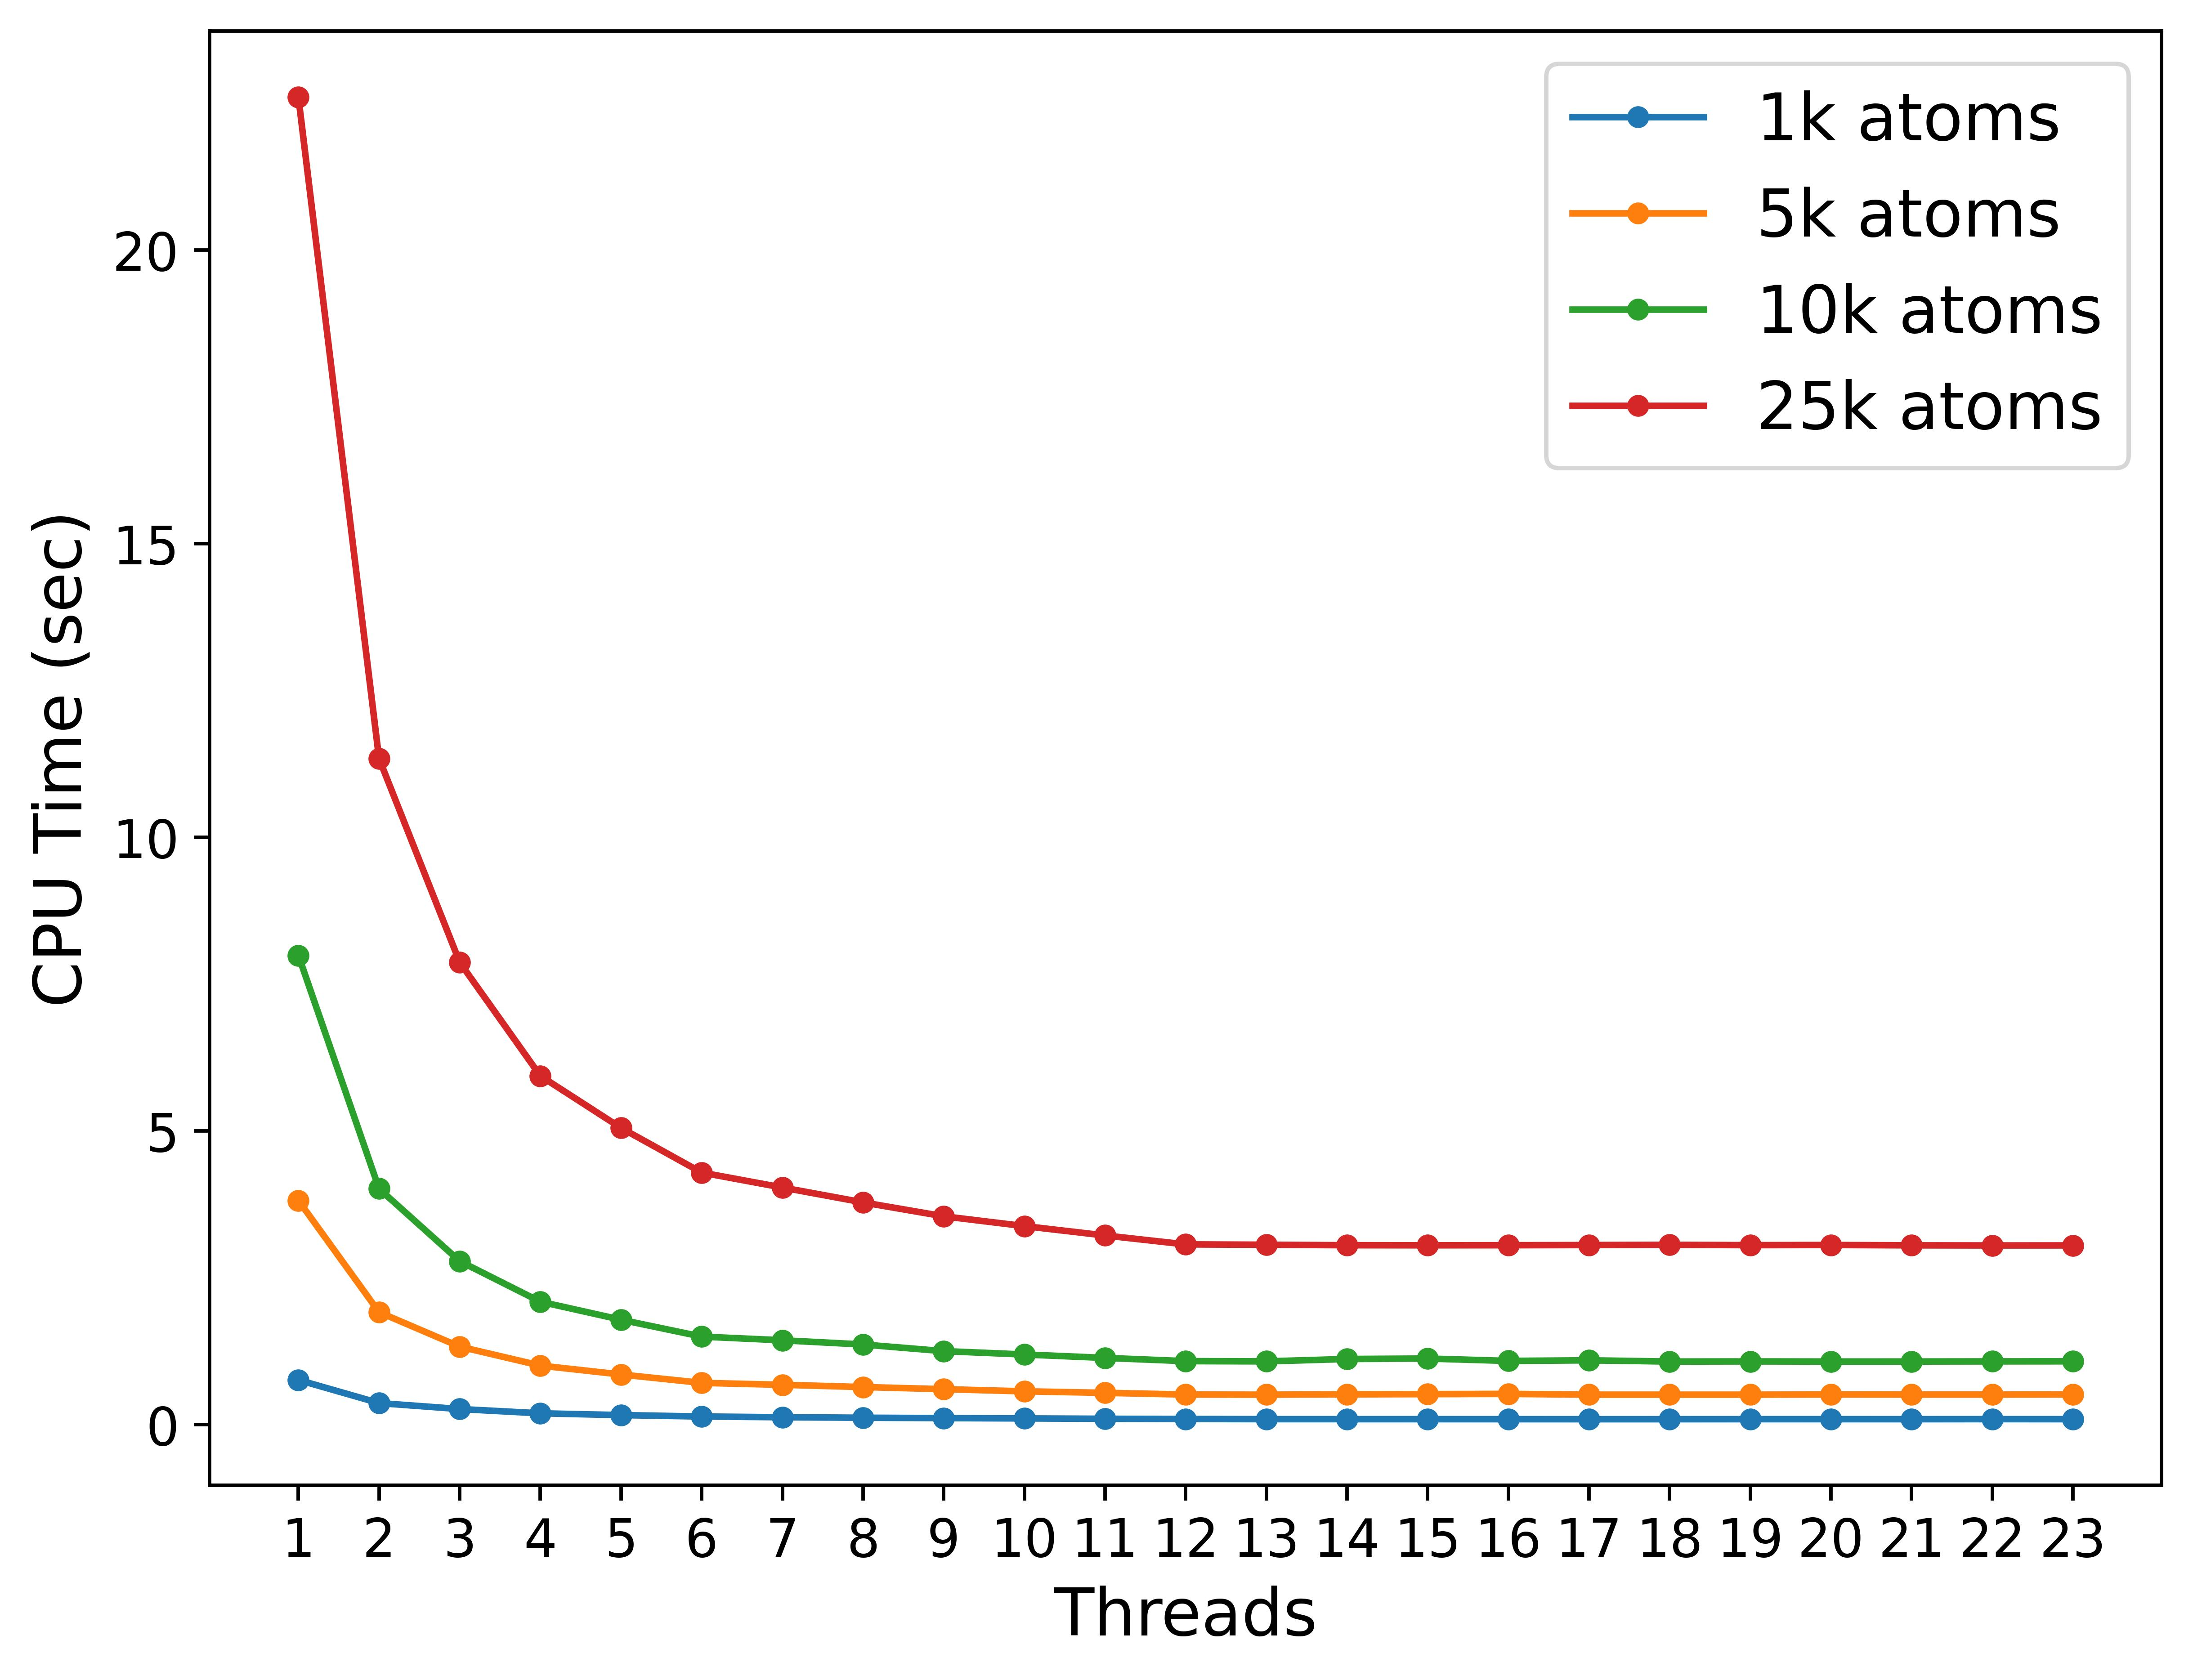
\includegraphics[width=0.75\textwidth]{images/threadstimetotal.jpg}
        \label{fig:thread-a}
    }\\[1ex]
    \subfigure[Total simulation time with SPME (grid: $64 \times 64 \times 512$, order: 8) across different thread counts.]{
        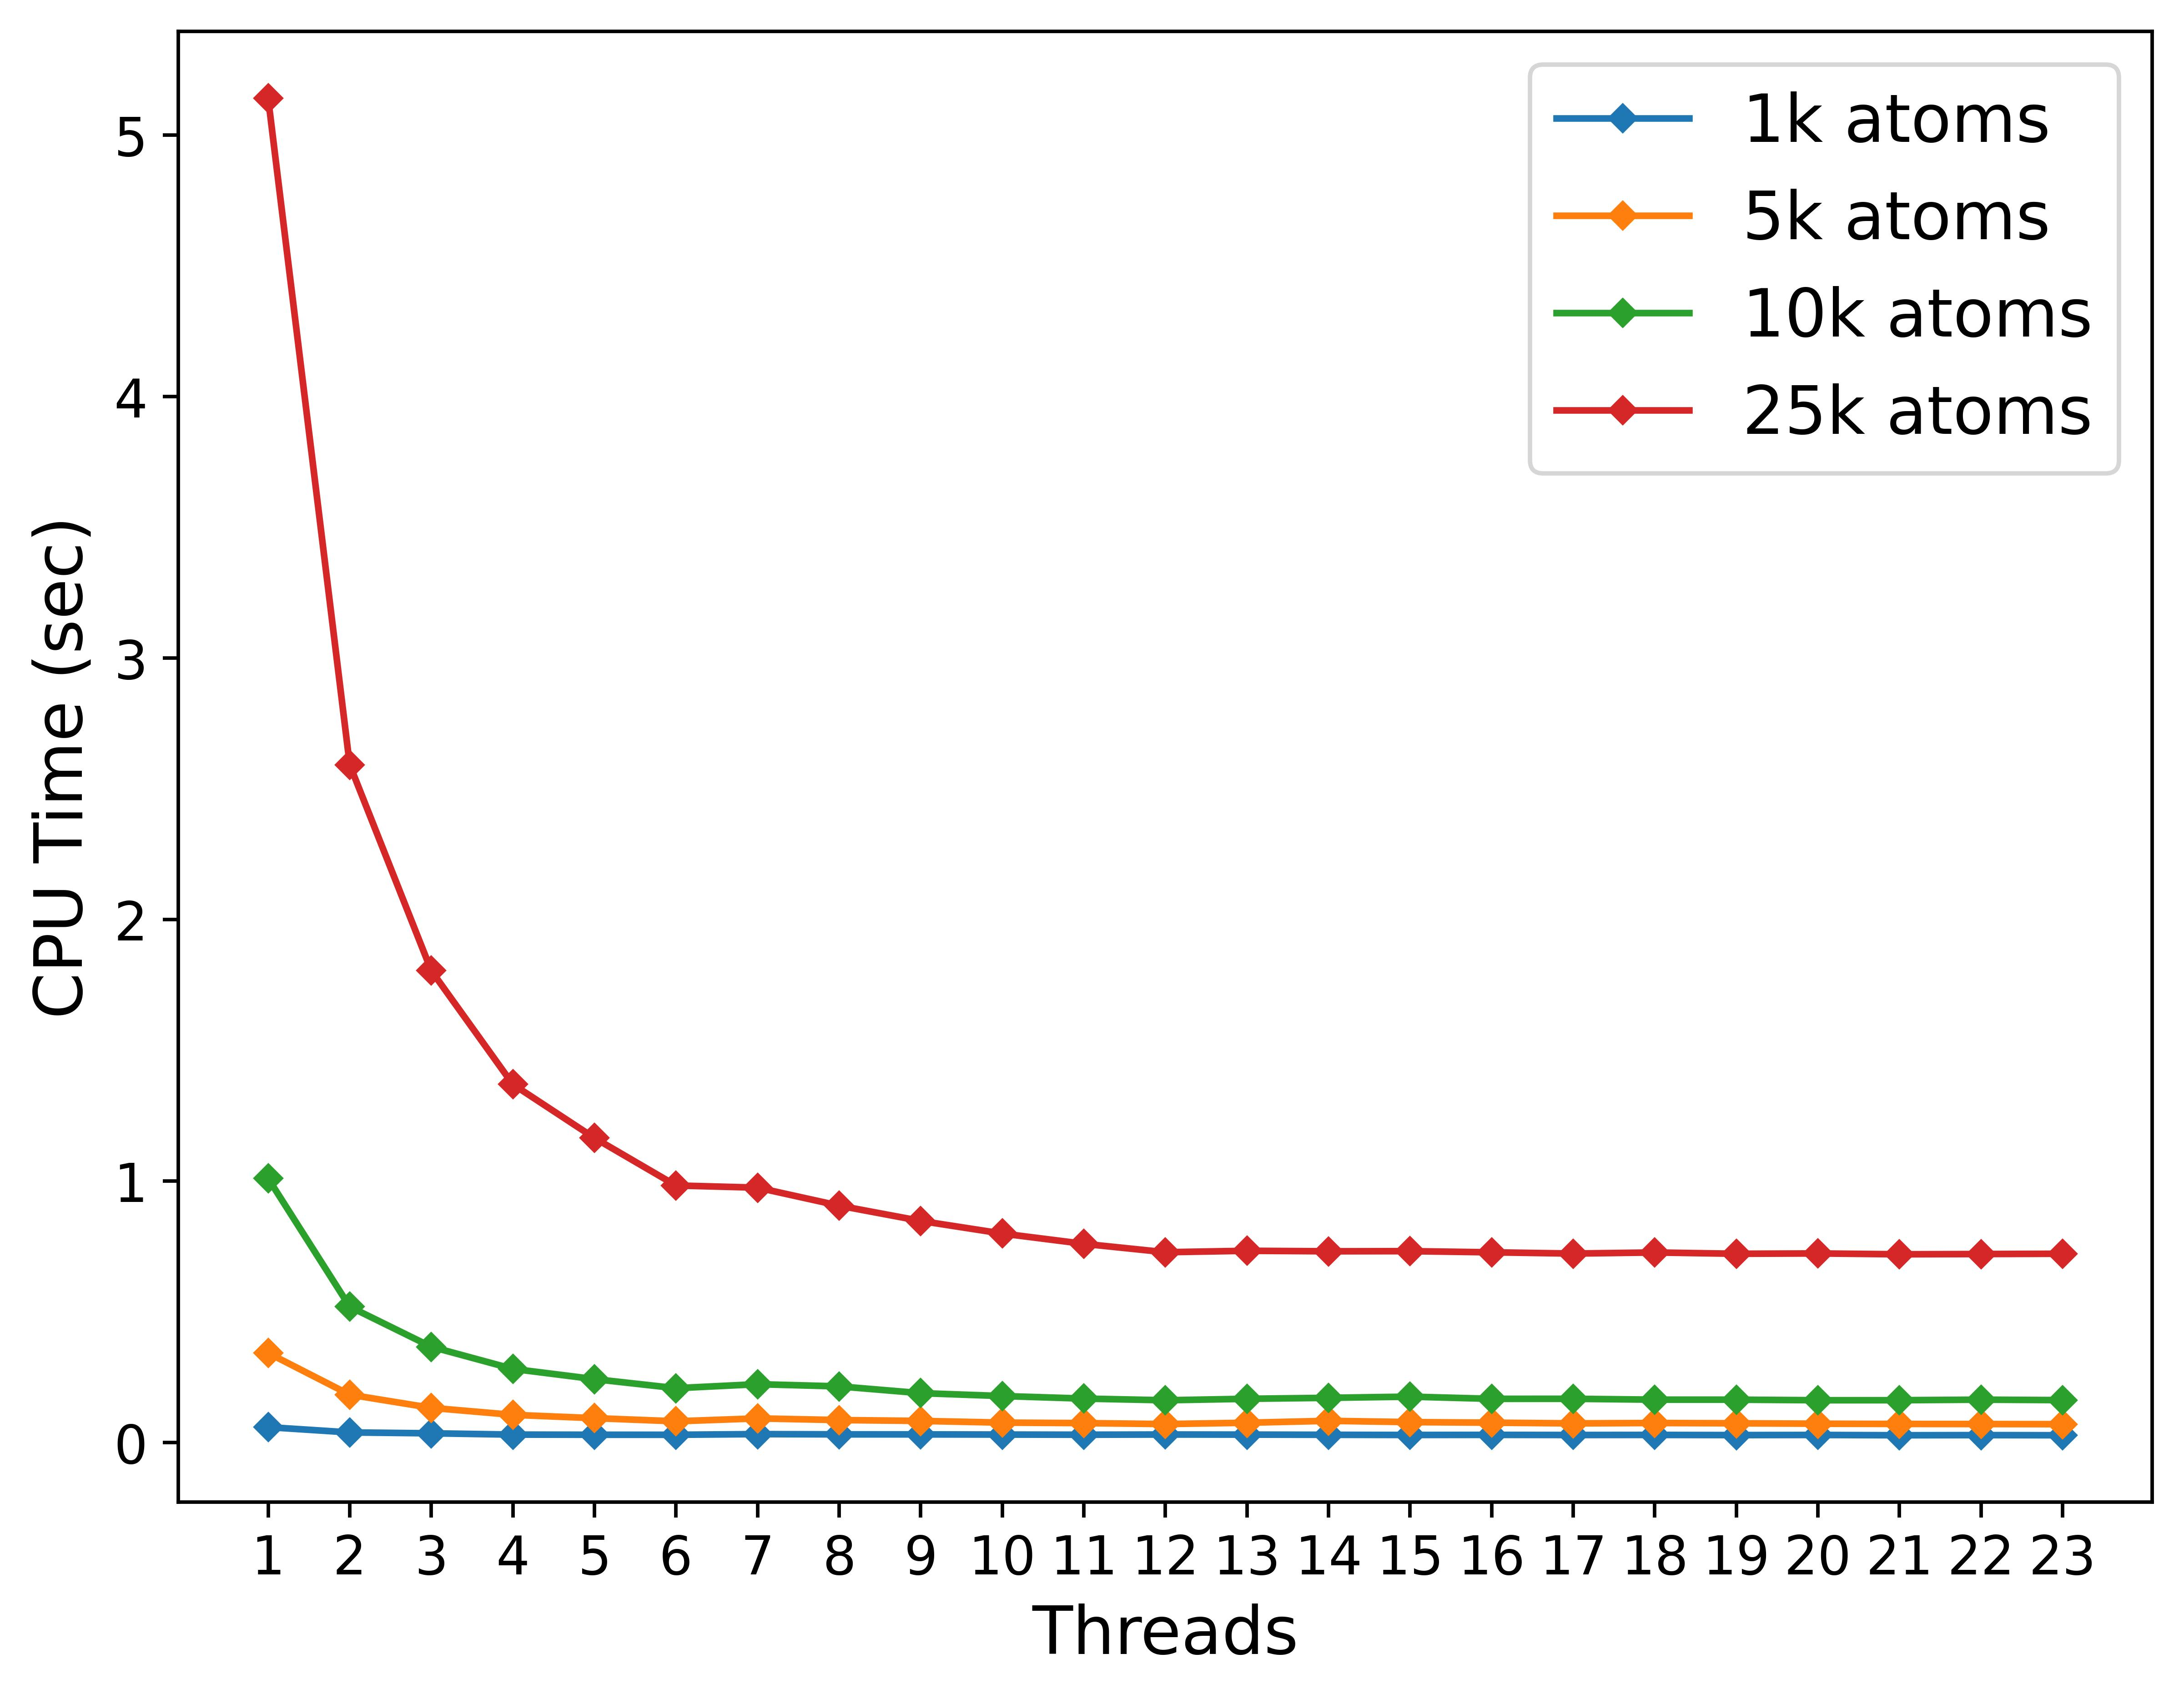
\includegraphics[width=0.75\textwidth]{images/threadstimeSPMEtotal.jpg}
        \label{fig:thread-b}
    }
    \caption{Comparison of threading performance.}
    \label{fig:threading}
\end{figure}

The results show a significant reduction in the execution times with increasing threads, up to 12, which corresponds to the total cores in the system. Beyond this point, the performance gains plateau. This behaviour shows the potential of parallelization within the bounds of the available hardware and achieving higher gain on better hardware.  

% \subsection{Implementation Correctness}

% \chapter{Numerical Evaluation: Accuracy and Efficiency}

\label{Chapter7} % Change X to a consecutive number; for referencing this chapter elsewhere, use \ref{ChapterX}

\lhead{Chapter 7. \emph{Numerical Evaluation: Accuracy and Efficiency}}
Calculations were performed on 12\textsuperscript{th} Gen Intel\textsuperscript{\textregistered} Core\texttrademark{} i5-12500~$\times$~12 core processor
we evaluated the computational efficiency and accuracy of our algorithm and compared it with PHL ewald and also with the method given by kawata et al.
The dimentions of the system were $L_x = L_y = L_z = 25$ \AA . The configuration of the systems were generated randomly using LAMMPS.

\section{Convergence}
We took a system of 10,000 Na and Cl ions in a 25 \AA box for our convergence benchmarking.
Based on our analysis for various gamma values, we calculated the reciprocal space energies for a given system and checked for the convergence of the sum. But due to very high $k_z$ values for the convergence this method becomes more expensive as compared to other older methods because for every iteration of $k_z$ to compute the energy the new structure factor $S(\vec G)$ is computed which increase the time complexity by $O(N)$, so now we will use the particle mesh ewald which doesn't depend on the $k_z$ loop as the bottleneck of that program is grid interpolation which is done outside the energy summation loop.
% \begin{figure}[htbp]
\begin{figure}[H]
    \centering
    \includegraphics[scale=0.4]{images/logerror_vs_kz_forreport.jpg}
    % \includegraphics[width=\linewidth]{images/logerror_vs_kz_forreport.jpg}
    \caption{Convergence of relative errors in $U_{LR}$ with $k_z$ for various values of $\gamma$.}
    \label{fig:result1}
\end{figure}
\section{Particle Mesh Ewald-Modified}
To enhance the efficiency of the calculations, the structure factor was computed using B-spline interpolation employing Fast Fourier Transforms (FFTs). The best accuracy and optimal time of our method+SPME is determined from the combination of gamma, order and grid. smaller the gamma, higher the grid points required for the interpolation. 
\section{Real Space Improvement}
The of the interpolation function gave around 15\% improvement in the calculation time. 
\begin{figure}[H]
    \centering
    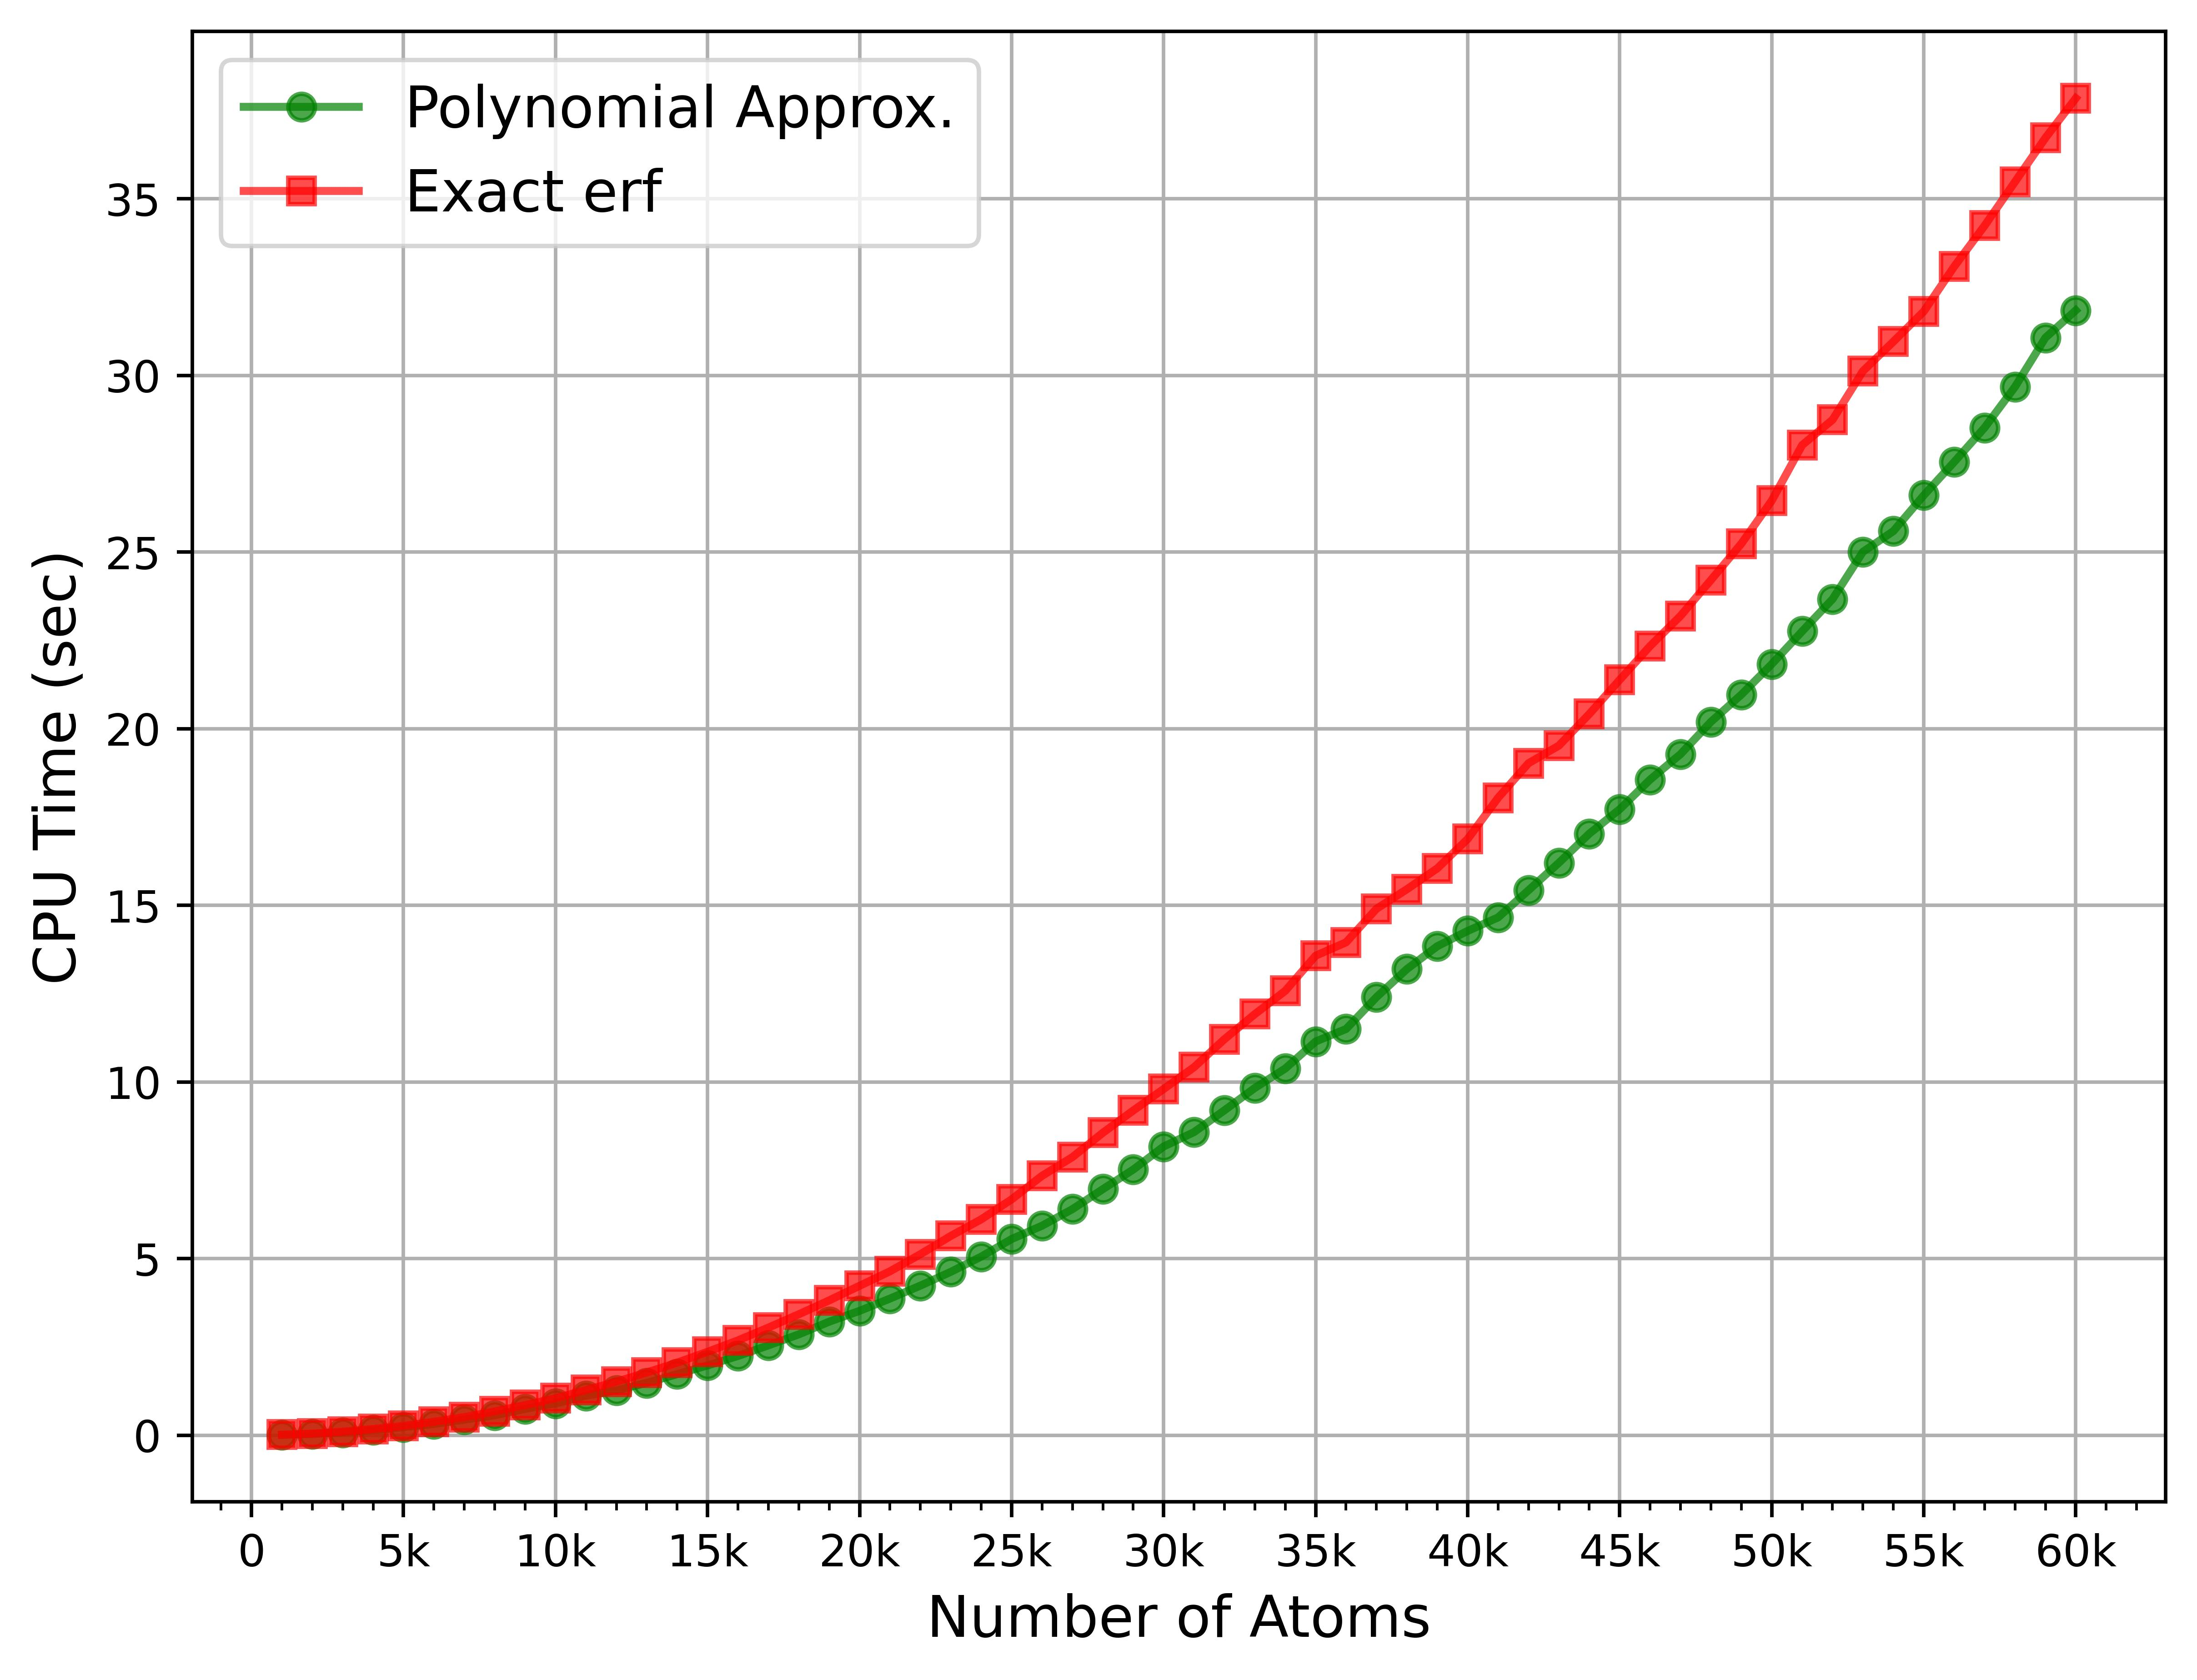
\includegraphics[width=0.75\linewidth]{images/realspaceopt.jpg}
    \caption{Enter Caption}
    \label{fig:enter-label}
\end{figure}
\begin{figure}[H]
    \centering
    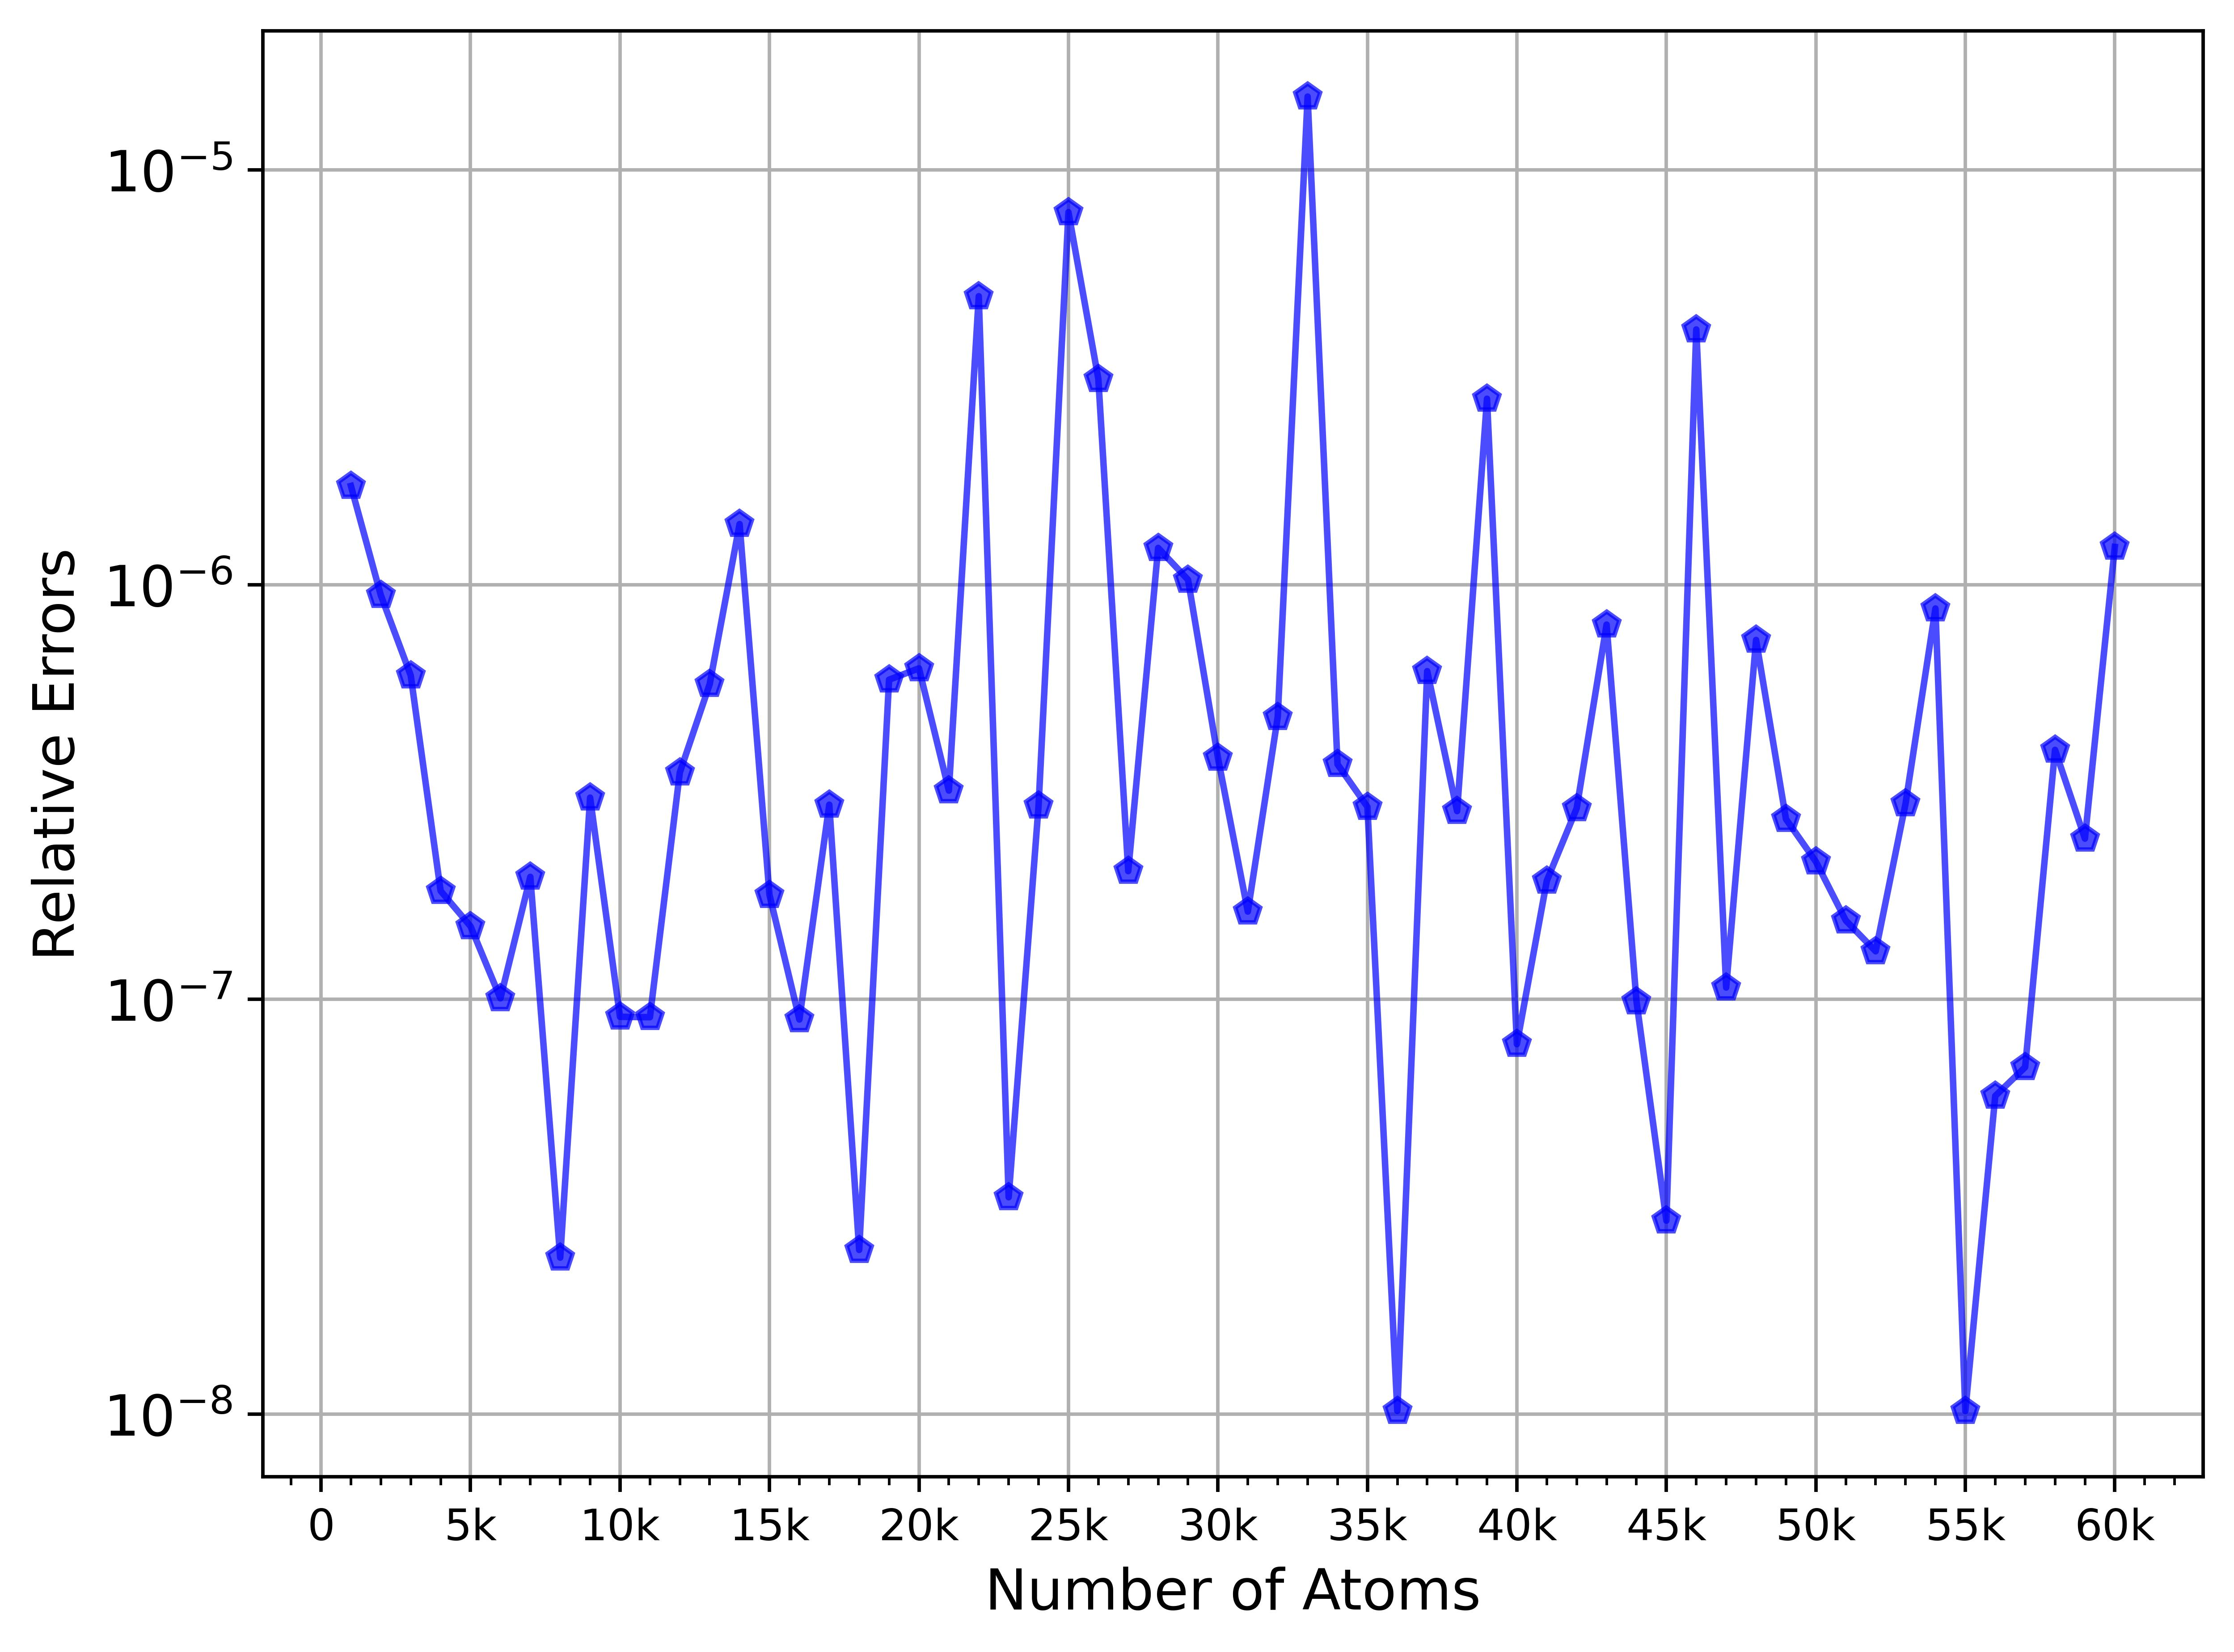
\includegraphics[width=0.75\linewidth]{images/realspaceopterrors.jpg}
    \caption{Enter Caption}
    \label{fig:enter-label}
\end{figure}
\section{Performance Scaling of the Ewald Method}
\subsection{Scaling Behaviour with System Size}
\begin{figure}[H]
    \centering
    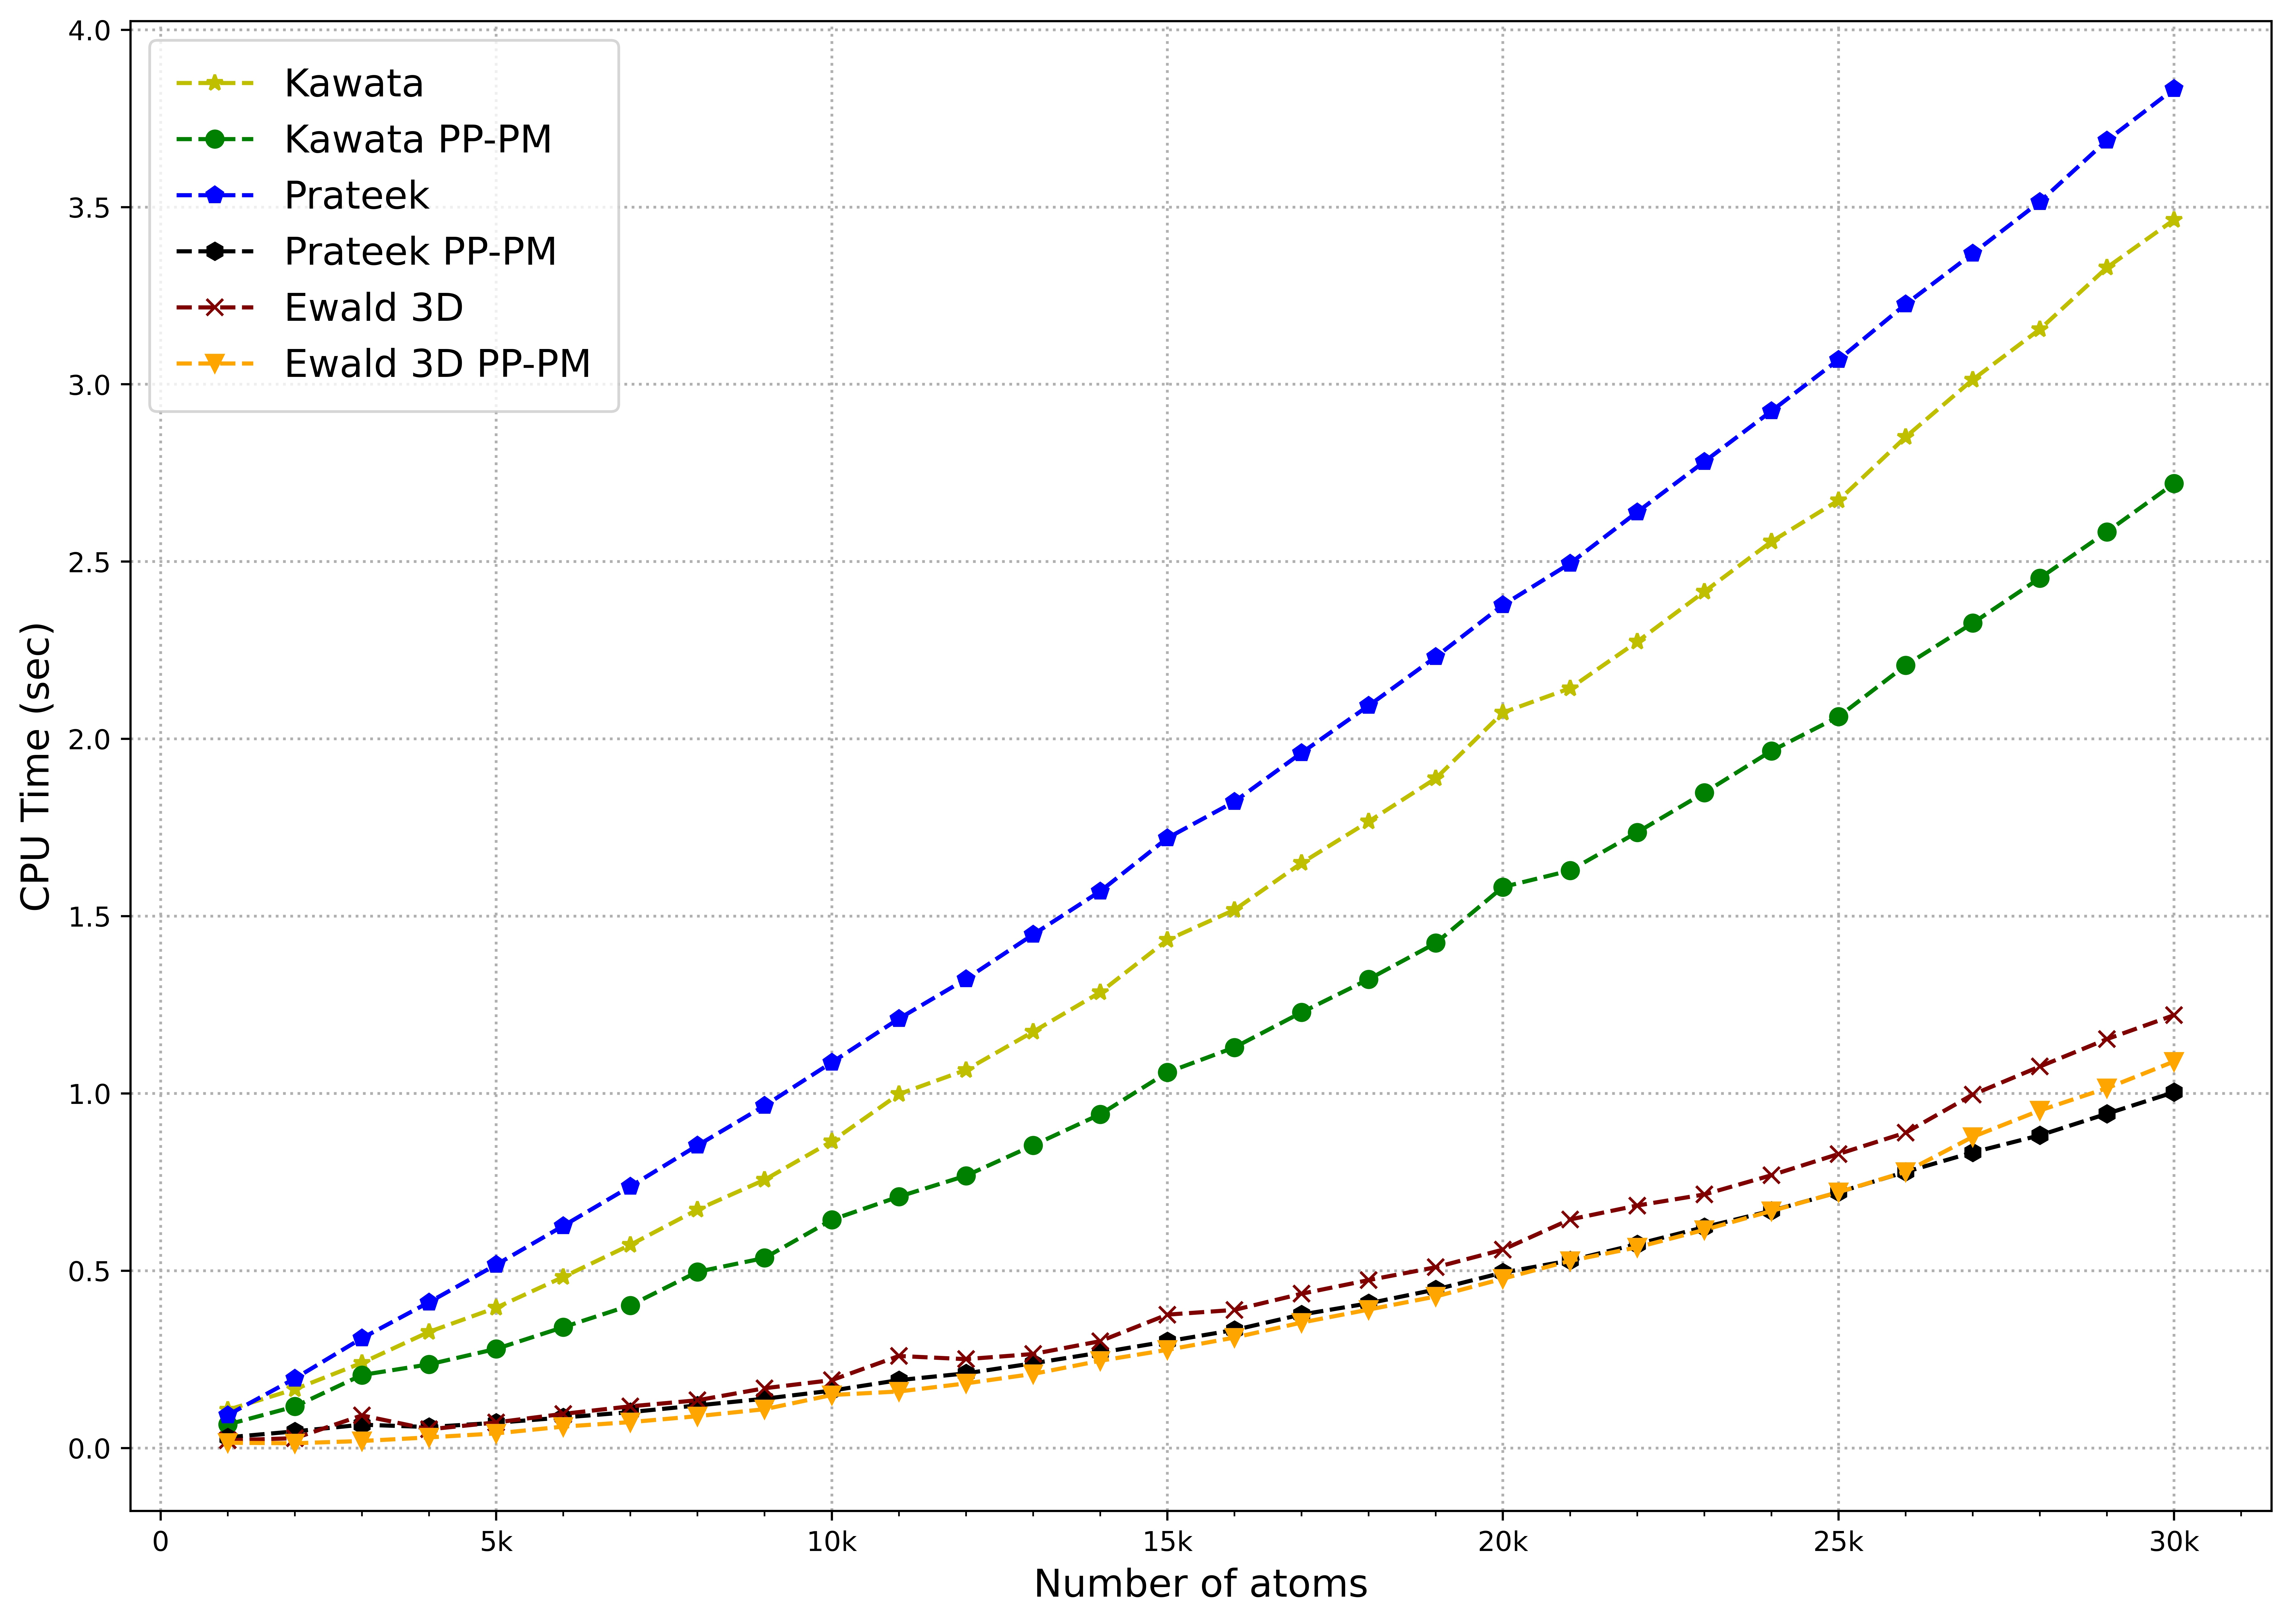
\includegraphics[width=\linewidth]{images/Result30k.jpg}
    \caption{Enter Caption}
    \label{fig:enter-label}
\end{figure}
\subsection{Parallel Efficiency via Multi-threading}
\begin{figure}[H]
    \centering
    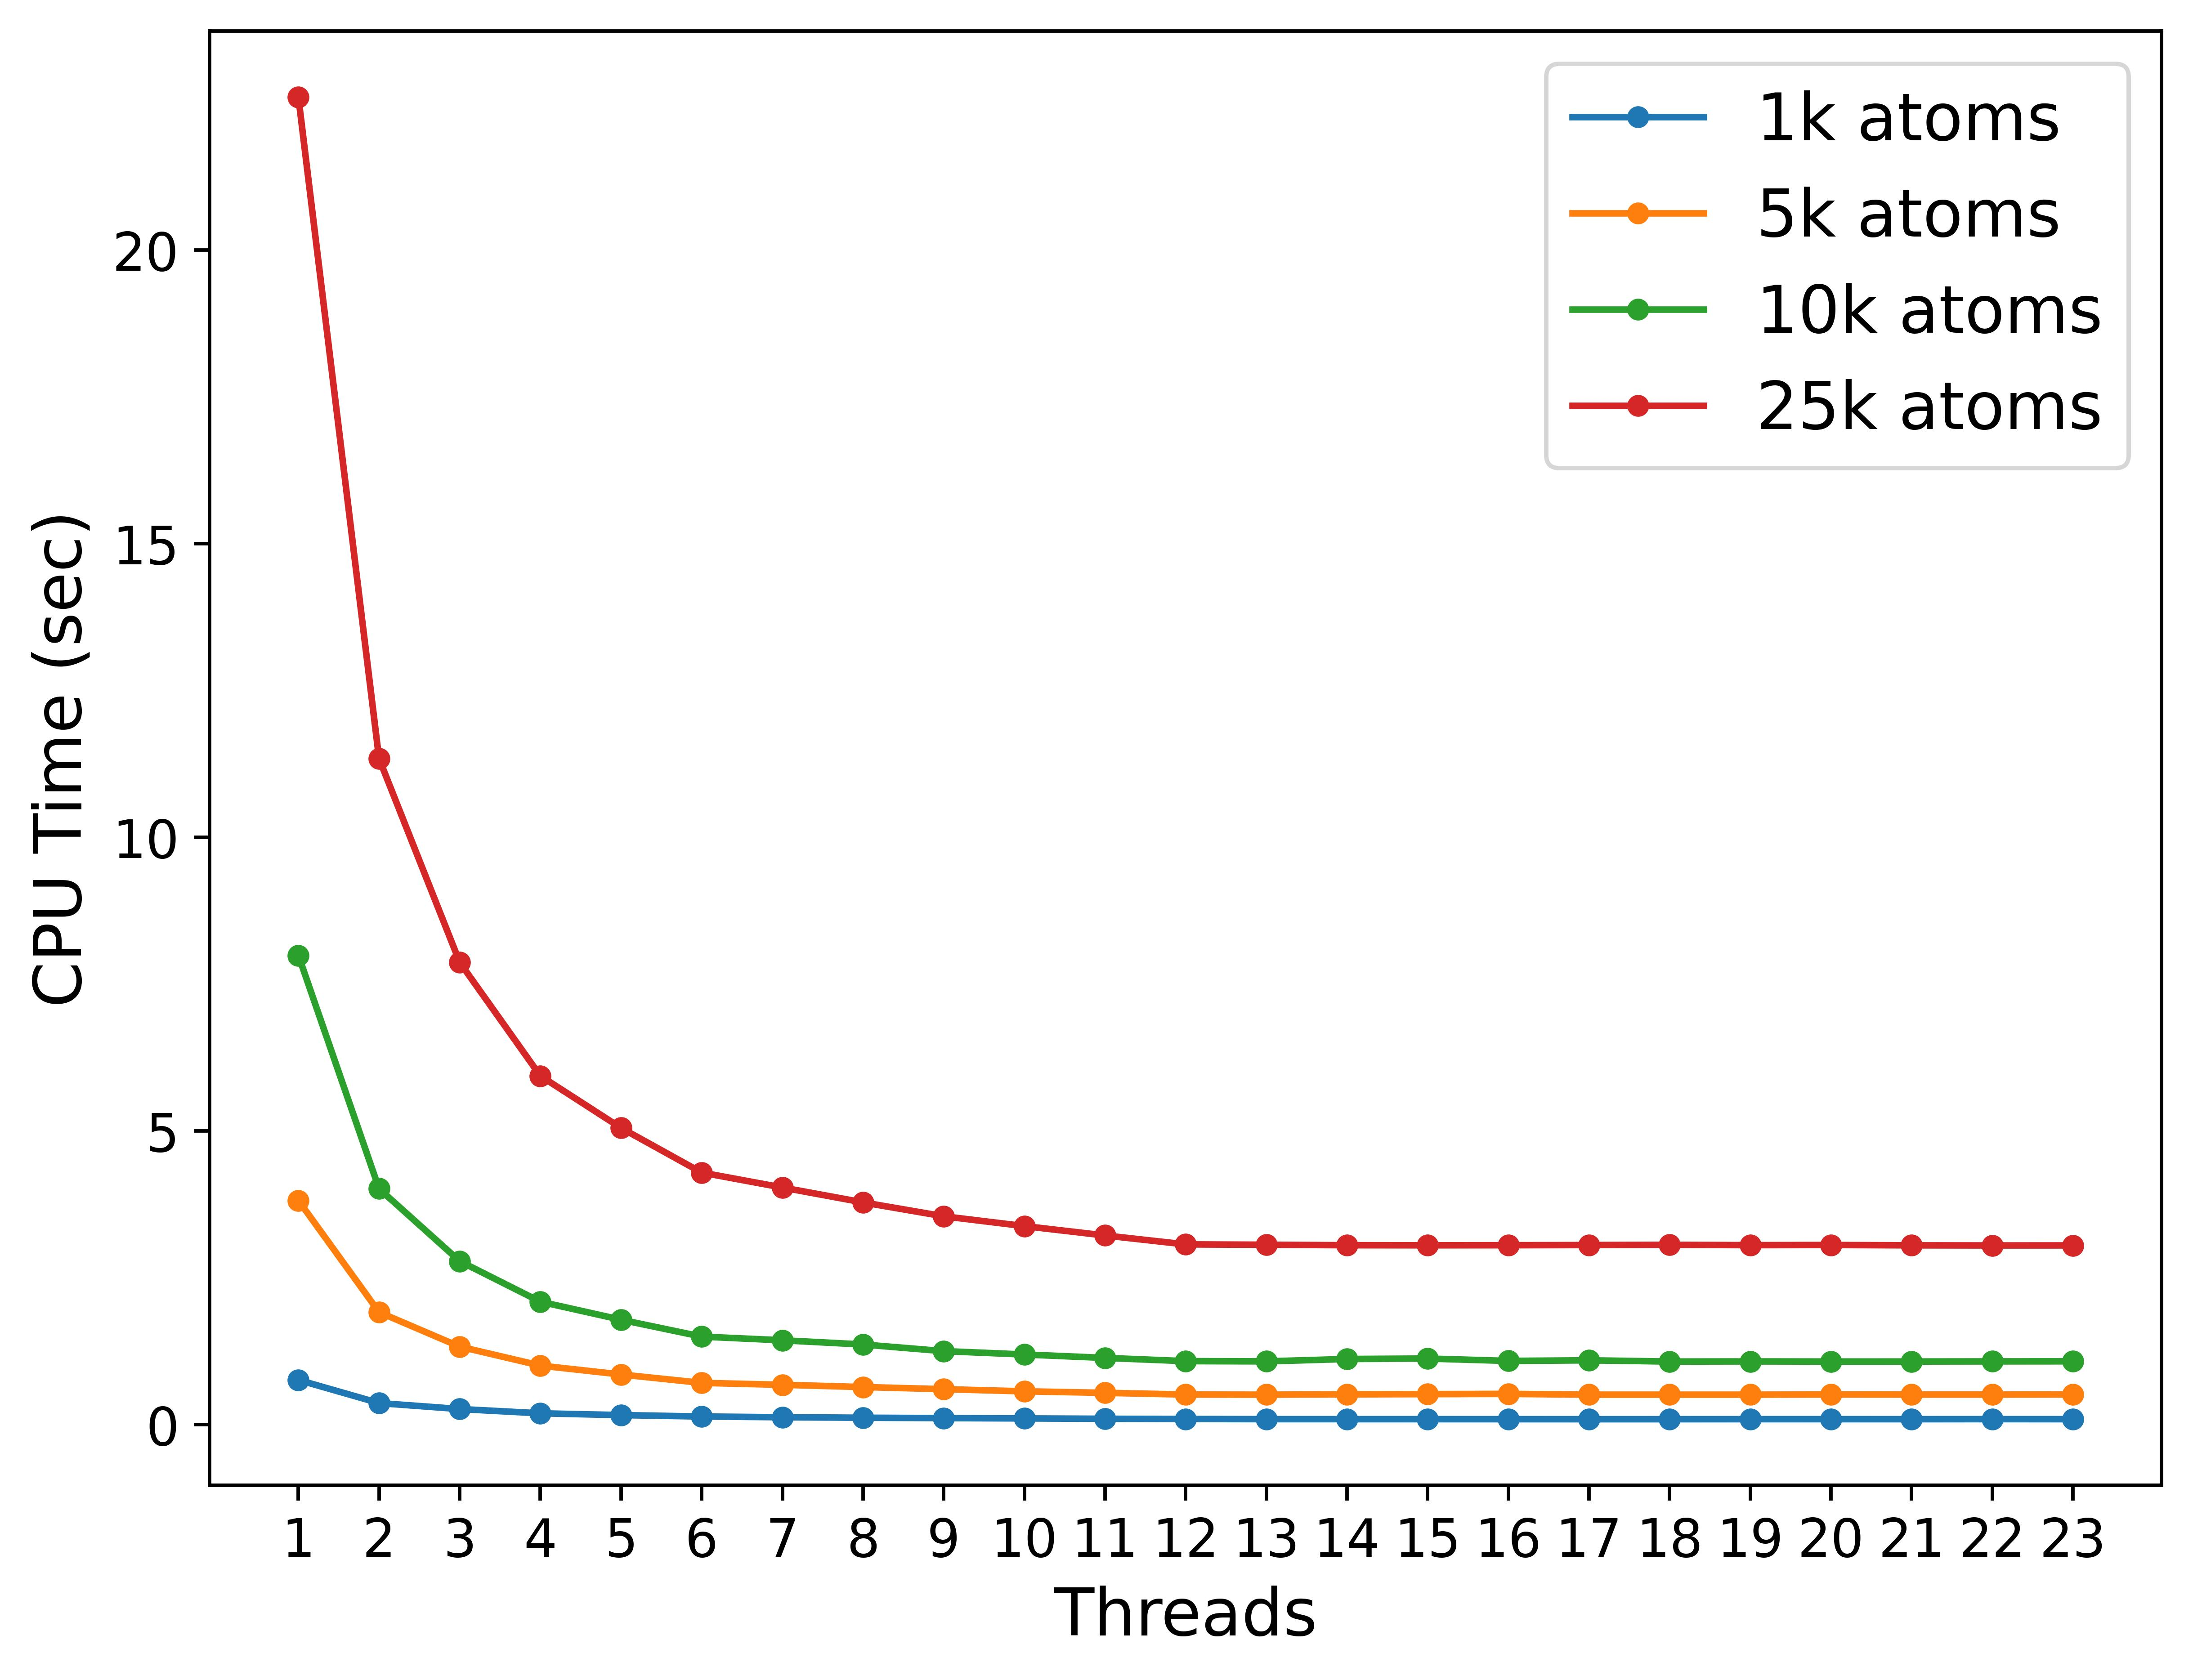
\includegraphics[width=0.7\linewidth]{images/threadstimetotal.jpg}
    \caption{Enter Caption}
    \label{fig:enter-label}
\end{figure}
\begin{figure}[H]
    \centering
    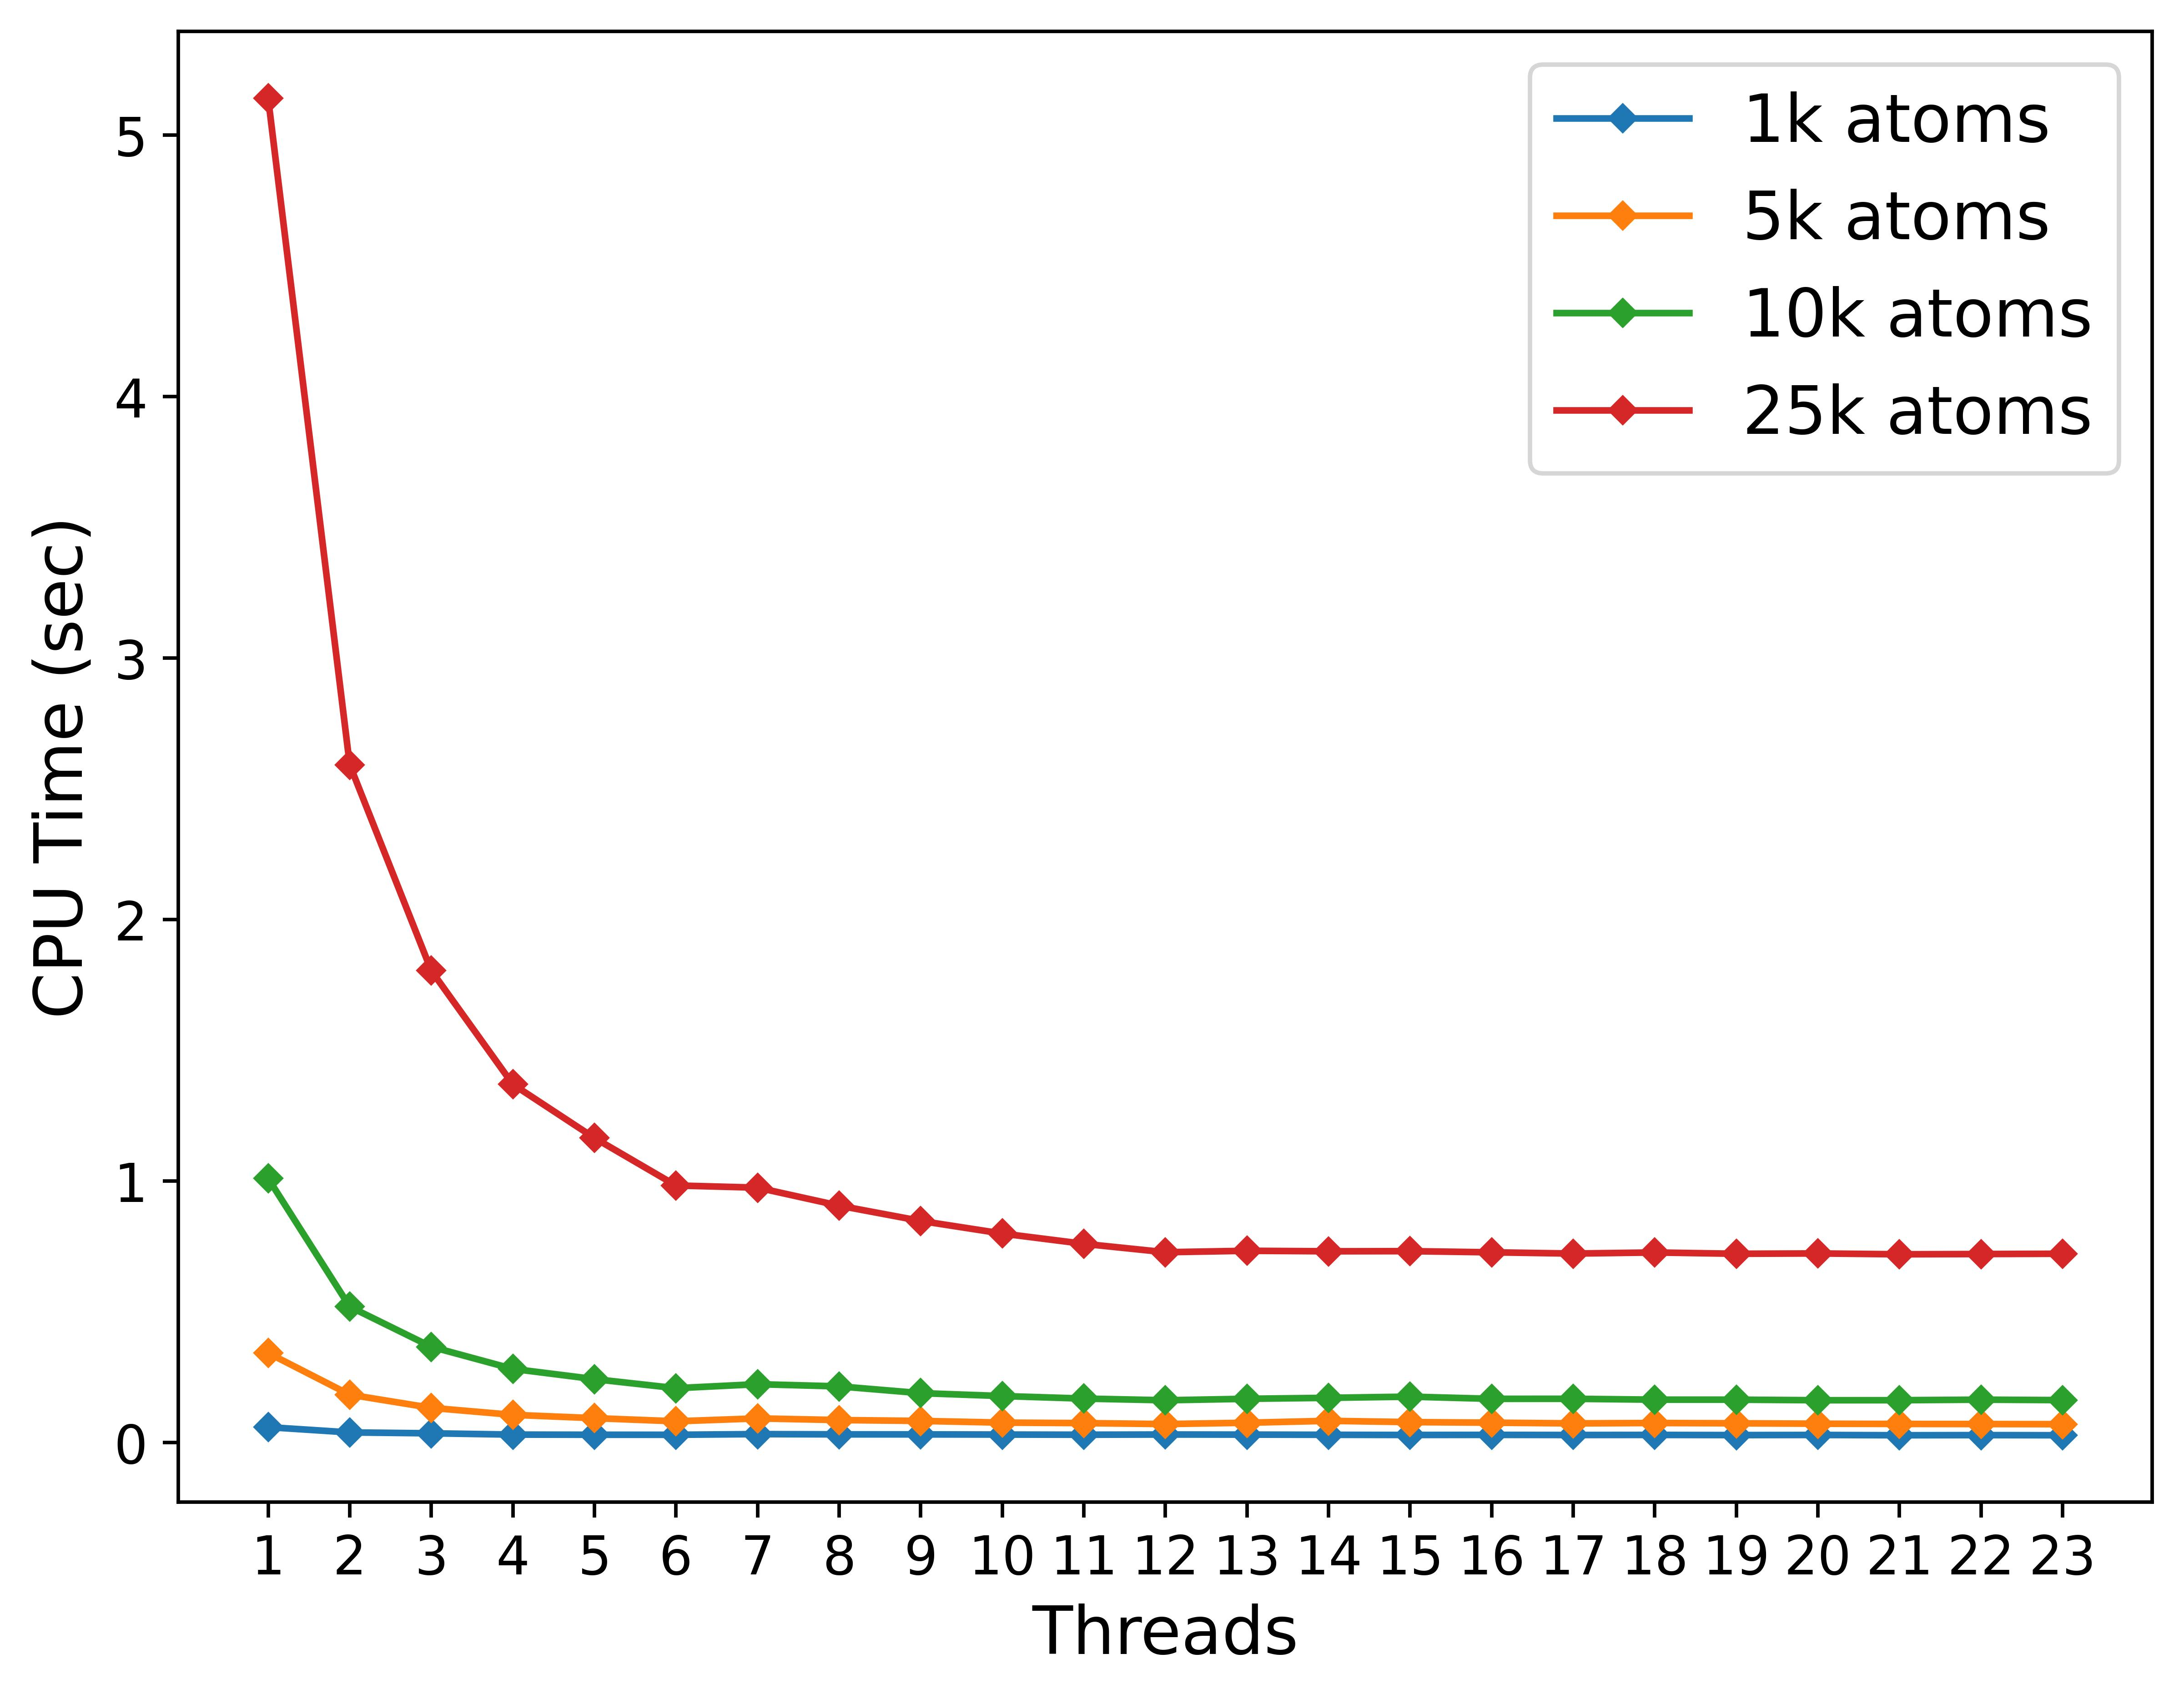
\includegraphics[width=0.7\linewidth]{images/threadstimeSPMEtotal.jpg}
    \caption{Enter Caption}
    \label{fig:enter-label}
\end{figure}
SPME configuration
gx = 64 
gy = 64
gz = 512
nxyz = 8

% \section{Summary}
% % Chapter Template

\chapter{Conclusions and future work}

\label{Chapter8} % Change X to a consecutive number; for referencing this chapter elsewhere, use \ref{ChapterX}

\lhead{Chapter 8. \emph{Conclusions and future work}}

\section{Conclusions}

\lipsum[1]

\textbf{Topic 1}

\begin{enumerate}
       
    \item \lipsum[1]

\end{enumerate}

\textbf{Topic 2}

\begin{enumerate}

    \item \lipsum[1]
     
\end{enumerate}

\section{Scope for future work}

\lipsum[1]. Some of these issues are listed:

\begin{enumerate}

    \item \lipsum[1]

\end{enumerate}


%----------------------------------------------------------------------------------------
%	THESIS CONTENT - APPENDICES
%----------------------------------------------------------------------------------------
\addtocontents{toc}{\vspace{2em}} % Add a gap in the Contents, for aesthetics
\appendix % Cue to tell LaTeX that the following 'chapters' are Appendices

% Include the appendices of the thesis as separate files from the Appendices folder
% Uncomment the lines as you write the Appendices

\chapter{Real to Fourier Space Transformation using Poisson Summation}
\label{AppendixA} 
\lhead{Appendix A. \emph{Real to Fourier Space Transformation using Poisson Summation}} 
Let us consider the following periodic functions defined along different spatial directions.
In the $x$-direction, we define the function $F(x)$ as:
\begin{flalign*}
    F(x) &= \sum_{{m_x}=-\infty}^{\infty}exp\left[-(x+m_xL_x)^2 t^2\right]
\end{flalign*}
and similarly, in the $z$-direction, the function $F(z)$ is given by:
\begin{flalign*}
    F(z) &= \sum_{{m_z}=-\infty}^{\infty}exp\left[-(z+m_zL_z)^2 t^2\right]\phi(z+m_zL_z) 
    % \\ &= \sum_{{m_z}=-\infty}^{\infty}exp\left[-(z+m_zL_z)^2 t^2\right]\left[\frac{1}{1+ exp(-\gamma(L_z(0.5+m_z)+z))} + \frac{1}{1+ exp(-\gamma(L_z(0.5-m_z)-z))} -1\right]
\end{flalign*}
where $L_x$ and $L_z$ denote the periodic lengths in the respective directions, $t$ is a constant, and $\phi(z)$ is a top-hat function.
Note that both functions $F(x)$ and $F(z)$ are periodic due to the infinite summation. Specifically,\[
F(x + L_x) = F(x) \quad \text{and} \quad F(z + L_z) = F(z).
\]
According to the Poisson summation formula, any periodic function with period \( L_z \) can be represented as a Fourier series. Hence, \( F(z) \) can be written as:
\begin{flalign*}
    F(z) &= \sum_{k=-\infty}^{\infty} C_k \hspace{1mm}exp(i\frac{2\pi k z}{L_z}) 
\end{flalign*}
where $C_k$ are constants. To obtain the values of $C_k$, we multiply each side by $exp(-i\frac{2\pi n z}{L_z})$ and integrate in z from 0 to $L_z$.
\begin{flalign*}
    \int_{0}^{L_z}C_{k_z}(t)dz &= \sum_{{m_z}=-\infty}^{\infty} \int_{0}^{L_z} dz\hspace{1mm}exp(-i\frac{2\pi n z}{L_z}) \hspace{1mm} exp\left[-(z+m_zL_z)^2 t^2\right] \, \phi(z+m_zL_z)
    % \\ &=\sum_{{m_z}=-\infty}^{\infty} \int_{0}^{L_z} dz\hspace{1mm}exp(-i\frac{2\pi n z}{L_z}) \hspace{1mm} exp\left[-(z+m_zL_z)^2 t^2\right]\times \\&\hspace{40mm}\left[\frac{1}{1+ exp(-\gamma(L_z(0.5+m_z)+z))} + \frac{1}{1+ exp(-\gamma(L_z(0.5-m_z)-z))} -1\right]
\end{flalign*}
Now substituting $s = z + mL_z$, and realizing that $exp(-i2\pi m n)=1$, we obtain
\begin{flalign}
   \nonumber C_{k_z}(t) &= \frac{1}{L_z}\sum_{{m_z}=-\infty}^{\infty} \int_{mL_z}^{(m+1)L_z} ds\, exp(-s^2t^2)\,exp(-i\frac{2\pi n s}{L_z}) \, \phi(s)
    \\ &=\frac{1}{L_z}\int_{-\infty}^{\infty}ds\, exp(-s^2t^2)\,exp(-i\frac{2\pi n s}{L_z}) \, \phi(s) \label{eq:ck}
\end{flalign}
Due to the complex form of $\phi(s)$ we cannot obtain a closed-form expression for the above integral and will have to solve using numerical methods.
% \colorbox{yellow}{no closed form integral expression} \\
To get the coefficients for the X and Y direction function, put $\phi(s) = 1$, and we can obtain the following closed-form expression for $C_{k_x}$ and $C_{k_y}$:
\begin{flalign*}
   C_{k_x}(t) &= \frac{1}{L_x}\sqrt{\frac{\pi}{t}} exp\left(\frac{-\pi^2k_x^2}{L_x^2t}\right)
\end{flalign*}
So our final expression to transform from real to reciprocal space would be:
\begin{flalign*}
    F(x) &=\sum_{{m_x}=-\infty}^{\infty}exp\left[-(x+m_xL_x)^2 t^2\right] = \frac{1}{L_x}\sqrt{\frac{\pi}{t}}\sum_{k_x=-\infty}^{\infty}exp\left(\frac{-\pi^2k^2}{L_x^2t}+i\frac{2\pi k_x x}{L_x}\right) 
    % \\ \sum_{{m_z}=-\infty}^{\infty}exp\left[-(z+m_zL_z)^2 t^2\right]\phi(z+m_zL_z) &=  \frac{1}{L_z}\sum_{k=-\infty}^{\infty}  \left[ \int_{-\infty}^{\infty}ds\, exp(-s^2t^2)\,exp(-i\frac{2\pi n s}{L_z}) \, \phi(s)\right]  exp\left(i\frac{2\pi kx}{L_x}\right)  
    \\ F(z) &=\sum_{{m_z}=-\infty}^{\infty}exp\left[-(z+m_zL_z)^2 t^2\right]\phi(z+m_zL_z) =  \sum_{k_z=-\infty}^{\infty}  C_{k_z}(t)  \, exp\left(i\frac{2\pi k_z z}{L_z}\right)  
\end{flalign*}
The value of $C_{k_z}(t)$ comes from equation \ref{eq:ck}
%\chapter{C/C++ Programs}
\label{AppendixB} % use \ref{AppendixB}
\lhead{Appendix B. \emph{C/C++ Programs}}

\section{2D Ewald}
    \subsection{Main file}
    \lstinputlisting[language=C]{CodeFiles/Ewald2D/main.cpp}
    
    \subsection{dist function}
    \lstinputlisting[language=C]{CodeFiles/Ewald2D/dist.cpp}
    
    \subsection{Real Space Energy function}
    \lstinputlisting[language=C]{CodeFiles/Ewald2D/real.cpp}
    
    \subsection{Self Energy function}
    \lstinputlisting[language=C]{CodeFiles/Ewald2D/self.cpp}
    
    \subsection{2D-EW}
    \textbf{Reciprocal Space Energy (k $=$ 0)}
    \lstinputlisting[language=C]{CodeFiles/Ewald2D/reci0.cpp}
    
    \textbf{Reciprocal Space Energy (k $\neq$ 0)}
    \lstinputlisting[language=C]{CodeFiles/Ewald2D/reci_integral.cpp}
    
    \subsection{2D-PME}
    \lstinputlisting[language=C]{CodeFiles/Ewald2D/reci_fft.cpp}
    
    \subsection{Helper functions}
    \lstinputlisting[language=C]{CodeFiles/Ewald2D/func.cpp}
    
    \subsection{New 2D Ewald Method}
        \subsubsection{Direct Ewald}
        \lstinputlisting[language=C]{CodeFiles/Ewald2D/New2DEwald.cpp}
        
        \subsubsection{Particle Mesh Adaptation}
        \lstinputlisting[language=C]{CodeFiles/Ewald2D/PM2DEwald.cpp}

        \subsubsection{Screening Factor Array}
        \lstinputlisting[language=C]{CodeFiles/Ewald2D/screen.cpp}
        
% \section{New Method for 2D Ewald}

%\input{Appendices/AppendixC}

\addtocontents{toc}{\vspace{2em}} % Add a gap in the Contents, for aesthetics

\backmatter

%----------------------------------------------------------------------------------------
%	BIBLIOGRAPHY
%----------------------------------------------------------------------------------------
\nocite{*}
\label{Bibliography}

\lhead{\emph{Bibliography}} % Change the page header to say "Bibliography"
\bibliographystyle{ieeetr} % Use the "custom" BibTeX style for formatting the Bibliography
\bibliography{Bibliography} % The references (bibliography) information are stored in the file named "Bibliography.bib"

\end{document}  